\documentclass[logos,hyperref,mainlanguage=english,morelanguage=french]{my-orsay-thesis}
%Text encoding and fonts
\usepackage[latin1]{inputenc}
\usepackage[T1]{fontenc}
\usepackage{amsmath}
\usepackage{mathrsfs}
\usepackage{cancel}
\usepackage{caption}
\usepackage{subcaption}
\usepackage{subcaption}
\usepackage{tikz}
\usepackage{graphicx}
% \bibliographystyle{unsrt}
\usepackage[hyperref=true,
            url=false,
            isbn=false,
            backref=true,
            maxcitenames=3,
            maxbibnames=100,
            block=none,
            style=trad-unsrt,
            backend=biber]{biblatex}
\bibliography{./bib/biblio}
\DefineBibliographyStrings{english}{%
    backrefpage  = {see p.}, % for single page number
    backrefpages = {see pp.} % for multiple page numbers
}
\usepackage[activate={true,nocompatibility},final,tracking=true,kerning=true,spacing=true,factor=1100,stretch=10,shrink=10]{microtype}
% activate={true,nocompatibility} - activate protrusion and expansion
% final - enable microtype; use "draft" to disable
% tracking=true, kerning=true, spacing=true - activate these techniques
% factor=1100 - add 10% to the protrusion amount (default is 1000)
% stretch=10, shrink=10 - reduce stretchability/shrinkability (default is 20/20)
\SetTracking{encoding={*}, shape=sc}{40}
\SetProtrusion{encoding={*},family={bch},series={*},size={6,7}}
              {1={ ,750},2={ ,500},3={ ,500},4={ ,500},5={ ,500},
               6={ ,500},7={ ,600},8={ ,500},9={ ,500},0={ ,500}}
\graphicspath{{./figures/}}
% \setlength{\parindent}{4em}
% \setlength{\parskip}{1em}
% \renewcommand{\baselinestretch}{2.0}
\DeclareTextSymbol{\degree}{T1}{6}
\definecolor{forestgreen}{rgb}{0.0, 0.27, 0.13}
%########################################################################
% Title page
%########################################################################
\author{Oscar Roberto \textsc{BLANCO GARC�A}}
\title{Beam dynamics in the final focus of the CLIC future linear collider project}
\title[english]{Dynamique du faisceau dans las section finale de focalisation du futur collissionneur lin�aire}
\keywords{Some keywords}
%Keywords for other languages languages
% \keywords[english]{Blabla, blabla, blabla, blabla, blabla, blabla, blabla}
%Order number of the thesis
\ordernumber{xxxx}
%Date of defense
\date{03/07/2015}
%You define the commission member list using \addcommissionmember (mandatory) with an optional role (eg: president, supervisor, etc...)
\addcommissionmember[Directeur de th�se]{Directeur de Recherche}{Philip}{Bambade}
\addcommissionmember[Co-encadrant]{Physicien au CERN}{Rogelio}{Tom�s}
\addcommissionmember[Examinateur]{Professeur}{Achille}{Stocchi}
\addcommissionmember[Rapporteur]{Professeur}{Jean-Marie}{De Conto}
\addcommissionmember[Rapporteur]{Professeur Associ�}{Nobuhiro}{Terunuma}
\addcommissionmember[Examinateur]{Professeur Associ�}{Toshiaki}{Tauchi}
%########################################################################
% Document start
%########################################################################
\begin{document}
%Print title NOW
\maketitle%
%Disable page numbering
\pagestyle{empty}
%########################################################################
% Multilingual abstracts
%########################################################################
% %French abstract:
% \begin{abstract}
% \begin{abstract}[english]
The exploration of new physics in the TeV scale with precision measurements requires lepton colliders providing high luminosities to obtain enough statistics for the data analysis. In order to achieve design luminosity values, linear colliders feature nanometer beam spot sizes at the Interaction~Point~(IP).\par
In addition to several effects affecting the luminosity, three main issues to achieve the beam size demagnification in the Final Focus Section (FFS) of the accelerator are the chromaticity correction, the synchrotron radiation effects and the correction of the lattice errors.\par
The current linear collider projects, CLIC and ILC, have lattices designed using the local or non-local chromaticity correction schemes. A new chromaticity correction scheme, called non-interleaved, is proposed to the local and non-local chromaticity corrections for CLIC. This lattice is designed and diagnosed, where the main issue in the current state of lattice design is the non-zero second order dispersion in the Final Doublet~(FD) region where a strong sextupole is used to correct the remaining geometrical components. It could be solved by cancelling the second order dispersion and its derivative before the FD.\par
The radiation effect can be evaluated by tracking particles through the lattice or by analytical approximations during the design stage of the lattices. In order to include both, radiation and optic parameters, during the design optimization process, two particular radiation phenomena are reviewed: the Oide effect~\cite{Oide} and the radiation caused by bending magnets~\cite{Sands}.\par
The analytical result of the radiation in bending magnets in~\cite{Sands} was generalized to the case with non-zero alpha and non-zero dispersion at the IP, required during the design and luminosity optimization process. The closed solution for one dipole and one dipole with a drift is compared with the tracking code PLACET~\cite{Placet}, resulting in the improvement of the tracking code results.\par% Finally the model validity for the FFS design is analyzed concluding an agreement within $\pm10\%$ between the theoretical contribution to beam size and the tracking.\par
In the Oide effect, radiation in the final quadrupole sets a limit on the vertical beamsize. Only for CLIC 3~TeV this limit is significant, therefore two possibilities are explored to mitigate its contribution to beam size: double the length and reduce the QD0 gradient, or the integration of a pair of octupoles before and after QD0.\par
% The best result with octupoles demonstrates vertical beam size reduction of $(4.3\pm0.5)$\%, with little or negative impact on luminosity. The correction scheme is currently limited by the phase advance and $\beta_y/\beta_x$ ratio between correctors. It may be possible to improve its performance by slicing QD0.\par
Part of the requirements of the FFS for new linear accelerators, in particular ILC, are tested in The Accelerator Test Facility (ATF). The beam size reduction using the local chromaticity correction is explored by an extension of the original design, called ATF2 with two goals: ({\textbf{goal 1}}) achieve 37~nm of vertical beam size at the IP and ({\textbf{goal 2}}) the stabilization of the IP beam position at the level of few nanometres. Since 2014 beam size of 44~nm are achieved as a regular basis at charges of about~$0.1\times10^{10}$ particules per bunch.\par
A set of three cavities (IPA, IPB and IPC), two upstream and one downstream of the nominal IP, were installed and are used to measure the beam trajectory in the IP region, thus providing enough information to reconstruct the bunch position and angle at the IP. These will be used to for beam stabilization and could detect beam drift/jitter beyond the tolerable margin and undetected optics mismatch affecting the beam size measurements.\par
The specifications required of 1~nm resolution over 10~$\mu$m dynamic range at $1.0\times10^{10}$ particules per bunch with the ATF2 nominal optics have not been yet achieved. The results of the studies in the vertical plane of the cavities calibration show linearity within 5\% over two orders of magnitude of signal attenuation. The minimum resolution achieved is just below 50~nm at~$0.4\times10^{10}$ particules per bunch with a set of electronics impossing a noise limit on resolution of 10~nm per cavity. The dynamic range is 10~$\mu$m at 10~dB attenuation and $0.4\times10^{10}$ particules per bunch, indicating the need to upgrade the electronics. The integration to the ATF tuning instruments is ongoing. Nonetheless, feedback has been tested resulting in reduction of beam jitter down to 67~nm, compatible with resolution.\par
Two improvements have been done on the system since this study. First, the horizontal and vertical planes can be analyzed simultaneouly, such that data can be checked for coupling from one plane to another. Second, filters are added to the system in order to reduce the effect of the mismatch between frequencies in the electronics down-mixing process.\par
\end{abstract}
% \end{abstract}
%Horizontal rule
\noindent\hspace*{0.35\textwidth}\hrulefill\hspace*{0.35\textwidth}\\[-\bigskipamount]
%English abstract:
\begin{abstract}[english]
\begin{abstract}[english]
The exploration of new physics in the TeV scale with precision measurements requires lepton colliders providing high luminosities to obtain enough statistics for the data analysis. In order to achieve design luminosity values, linear colliders feature nanometer beam spot sizes at the Interaction~Point~(IP).\par
In addition to several effects affecting the luminosity, three main issues to achieve the beam size demagnification in the Final Focus Section (FFS) of the accelerator are the chromaticity correction, the synchrotron radiation effects and the correction of the lattice errors.\par
The current linear collider projects, CLIC and ILC, have lattices designed using the local or non-local chromaticity correction schemes. A new chromaticity correction scheme, called non-interleaved, is proposed to the local and non-local chromaticity corrections for CLIC. This lattice is designed and diagnosed, where the main issue in the current state of lattice design is the non-zero second order dispersion in the Final Doublet~(FD) region where a strong sextupole is used to correct the remaining geometrical components. It could be solved by cancelling the second order dispersion and its derivative before the FD.\par
The radiation effect can be evaluated by tracking particles through the lattice or by analytical approximations during the design stage of the lattices. In order to include both, radiation and optic parameters, during the design optimization process, two particular radiation phenomena are reviewed: the Oide effect~\cite{Oide} and the radiation caused by bending magnets~\cite{Sands}.\par
The analytical result of the radiation in bending magnets in~\cite{Sands} was generalized to the case with non-zero alpha and non-zero dispersion at the IP, required during the design and luminosity optimization process. The closed solution for one dipole and one dipole with a drift is compared with the tracking code PLACET~\cite{Placet}, resulting in the improvement of the tracking code results.\par% Finally the model validity for the FFS design is analyzed concluding an agreement within $\pm10\%$ between the theoretical contribution to beam size and the tracking.\par
In the Oide effect, radiation in the final quadrupole sets a limit on the vertical beamsize. Only for CLIC 3~TeV this limit is significant, therefore two possibilities are explored to mitigate its contribution to beam size: double the length and reduce the QD0 gradient, or the integration of a pair of octupoles before and after QD0.\par
% The best result with octupoles demonstrates vertical beam size reduction of $(4.3\pm0.5)$\%, with little or negative impact on luminosity. The correction scheme is currently limited by the phase advance and $\beta_y/\beta_x$ ratio between correctors. It may be possible to improve its performance by slicing QD0.\par
Part of the requirements of the FFS for new linear accelerators, in particular ILC, are tested in The Accelerator Test Facility (ATF). The beam size reduction using the local chromaticity correction is explored by an extension of the original design, called ATF2 with two goals: ({\textbf{goal 1}}) achieve 37~nm of vertical beam size at the IP and ({\textbf{goal 2}}) the stabilization of the IP beam position at the level of few nanometres. Since 2014 beam size of 44~nm are achieved as a regular basis at charges of about~$0.1\times10^{10}$ particules per bunch.\par
A set of three cavities (IPA, IPB and IPC), two upstream and one downstream of the nominal IP, were installed and are used to measure the beam trajectory in the IP region, thus providing enough information to reconstruct the bunch position and angle at the IP. These will be used to for beam stabilization and could detect beam drift/jitter beyond the tolerable margin and undetected optics mismatch affecting the beam size measurements.\par
The specifications required of 1~nm resolution over 10~$\mu$m dynamic range at $1.0\times10^{10}$ particules per bunch with the ATF2 nominal optics have not been yet achieved. The results of the studies in the vertical plane of the cavities calibration show linearity within 5\% over two orders of magnitude of signal attenuation. The minimum resolution achieved is just below 50~nm at~$0.4\times10^{10}$ particules per bunch with a set of electronics impossing a noise limit on resolution of 10~nm per cavity. The dynamic range is 10~$\mu$m at 10~dB attenuation and $0.4\times10^{10}$ particules per bunch, indicating the need to upgrade the electronics. The integration to the ATF tuning instruments is ongoing. Nonetheless, feedback has been tested resulting in reduction of beam jitter down to 67~nm, compatible with resolution.\par
Two improvements have been done on the system since this study. First, the horizontal and vertical planes can be analyzed simultaneouly, such that data can be checked for coupling from one plane to another. Second, filters are added to the system in order to reduce the effect of the mismatch between frequencies in the electronics down-mixing process.\par
\end{abstract}
\end{abstract}
\pagebreak
% %German abstract:
% \begin{abstract}[german]
% \dummytext
% \end{abstract}
%Horizontal rule
\noindent\hspace*{0.35\textwidth}\hrulefill\hspace*{0.35\textwidth}\\[-\bigskipamount]
%########################################################################
% Acknowledgments
%########################################################################
\pagebreak\strut\newpage
\section*{Remerciements}
%Put the text vertically centered
\vfill
This is the night of the 10th of april 2015.\par
I'm at Gen\`eve and I've been just been kicked out from La Petite Reine because the place was closing :'D, as if I care. After two beers here are my deepest acknowledgements:
From the begining...\par
My acknowledgement to Davide, the only person who has been cool every time I talk to him. My deepest acknowledgements to Alex, I wonder how the ILC course would be if I hadn't a person to talk about how people in relationships are like airplains ... some take off in very small tarmacs, like helicopters, some others need a large starting to take off.\par
My acknowledgements to Nuria who is the most constant person in my life during the last 3 years. I hope she has got something good for her life from my way of living. My acknowledgements to Julia, the russian ... waaaaw, life feels hot and nice when you speak to her. My acknowledgement to Hector, that guy is going to have his signature in the world when CLIC-like lattices were built, I want to say that we admire Carl Sagan equally... I thought it would never happen. I want to acknowledge Javier, he is the person who get me into accelerators and it is the only subject I've been looking forward to do things for during the last 10 years. I want to send an special acknowledge to Marcin, the thrill of changing every day for our own sake is what moves us, I would like to have his energy to do stuff, cheers my friend. And now, Tenar the spanish girl who appeared in the moment I most enjoyed it. Tenar, my life and heart is always happy when I hear from you. My biggest love during all these years, Claire. I don't know why, but that is probably the reason why my heart keeps beating when no one is around.\par
I want to thank Rogelio my director in CERN, the dynamics of his day to day is so dedicated to inspire people. Now, Philip, my director at LAL who is the person who stands for all what is right... I always admire how clear the world is for him. Of course, Andrea and Daniel, you are also here ! Daniel, the guy who knows everything about everything, so mind blowing. And Andrea, with whom would I talk about rare films and work at the same time... of course, only Andrea.\par
Finally, to all readers. Precisely today I wanted to be with Claire in the sunny afternoon, and this document kept me away from doing so. It is the moment to get right to the point, clear and neat. I know that Claire is fine, she always is... damn I love that girl.\par
All this is because of you, the reader.\par
N.B. Of course there has been some up and downs, but who cares. Time to flight !
\vfill
\newpage
%########################################################################
% Contents
%########################################################################
\strut\newpage
\microtypesetup{protrusion=false}
\tableofcontents
\listoffigures
\listoftables
\microtypesetup{protrusion=true}
\newpage
%########################################################################
% Introduction
%########################################################################
%Enable page numbering
\pagestyle{fancy}
\chapter*{Introduction}
\addcontentsline{toc}{chapter}{Introduction}
The triumph of the 20th century particle physics was the development of the Standard Model. Experiments determined the particle constituents of ordinary matter, and identified four forces binding matter and transforming it from one form to another. This success leads particle physicist to address even more fundamental questions, and explore deeper mysteries in science.\par
The Standard Model includes a third component beyond particles and forces, the Higgs mechanism. The Higgs mechanism permeates the universe, giving mass to the particles, and breaking the electro-weak force in two, the electromagnetic and the weak forces.\par
\begin{figure}[!hbt]
\centering
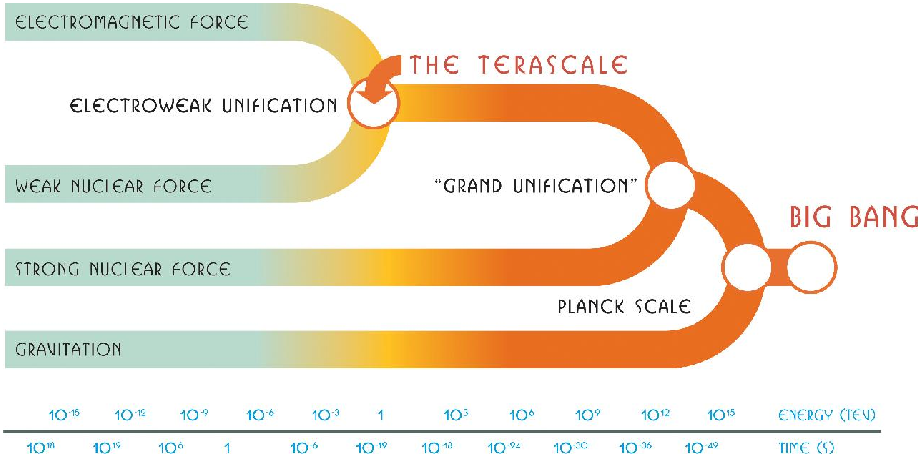
\includegraphics[scale=0.8,angle=0]{energyforce.pdf}\caption{The electromagnetic and electro-weak forces unify at the Terascale.}\label{f:energyforce}
\end{figure}
Experiments in the Terascale could test the idea that fundamental forces originate from a single unified force, see Fig. \ref{f:energyforce}, and search for evidence of a related unified origin of matter involving supersymmetry. They could distinguish among patterns of phenomena to judge different unification models, providing a telescopic view of the ultimate unification.\par
% \section*{The exploration of high energy physics}
% \addcontentsline{toc}{section}{The exploration of high energy physics}
There are two ways to explore the subatomic world, the first is to go to higher energy to discover new particles and measure their properties, the second is to increase the precision of the measurements to detect rare processes and make detailed studies.\par
The LHC allows the exploration of the electroweak symmetry breaking mechanism and other physical phenomena at the TeV scale, like the CP violation problem, the quark gluon plasma at the search of new physics beyond the Standard Model such as supersymmetry (SUSY) among others. The future linear collider beam energy will be determined by the LHC discoveries.\par
\textbf{Higgs searches:} The 4th of July of 2012, in a seminar held at CERN, the collaborations of the Experiments CMS and ATLAS presented an update of the Higgs of the Higgs searches status. At a confidence level of 4.9$\sigma$ for CMS \cite{TheCMSCollaboration21122012}, and 5.1$\sigma$ for ATLAS \cite{TheATLASCollaboration21122012} from the Higgsless Standard Model, signals of a boson with a mass around $m_h=125$~GeV were found with a strong spin-0 indication and coupling parameters consistent with the properties of the Standard Model Higgs Particle. First results on various rare production decay modes have been obtained but more data is needed to observe these models. Many analyses are ongoing and more updates are constantly presented.\par
\textbf{Heavy Flavour and CP Violation:} The experiments of the LHC, led by the LHCb, have carried out several important findings and measurements in the heavy flavour sector. New previously unobserved states have been observed for the very first time during the last years like the states $X_b$, $\Xi_a$ and $\Lambda_s^0$. Also the measurement of the quantum numbers of the states $X(3872)$ with $J^{PC}=1^{++}$, have been determined to the 8$\sigma$ level. The CP violation of the oscillation in D and B mesons have been measured to the 9.1$\sigma$ confidence level discovering the same violation in $B_s$ systems. The CP angle $\gamma$ is known with a precision without precedents ($\gamma=(67\pm12)$\textdegree). Finally, some very rare decays like $B_s\rightarrow\mu^+\mu^-$, $B^0\rightarrow K^*\mu^+\mu^-$ and $D_s^+\rightarrow\pi^+\mu^+\mu^-$ have been observed, with possible implications on the analysis of new physics.\par
\textbf{Quark-gluon Plasma:} The quark-gluon plasma is produced in ultra-relativistic heavy ion collisions. The conditions observed at the LHC experiments (ALICE, ATLAS and CMS) are in agreement with the observations carried out at RHIC. It has been confirmed that the hydrodynamics model helps in the understanding of the behaviour of the processes occurred during the collision. It is still far from being completely understood.\par
\textbf{SUSY and Dark Matter searches:} One of the problem that arises is the stabilization of the Higgs mass and its divergence when quantum divergence is considered. The solution involves a new principle of nature called supersymmetry (SUSY), a new symmetry that unifies bosons and fermions. After data collected during 2011 and 2012, SUSY searches at the LHC did not find any evidence of any light superpartner (squark or gluino) and it has pushed their mass limits beyond 1~TeV with the constrained model~\cite{Kraml:2012er}.\par
\vspace*{0.6cm}
The Second run of the LHC at 13~TeV will provide more information about the physics at high energies.\par

\section*{Circular or linear colliders}
\addcontentsline{toc}{section}{Circular or linear colliders}
Higher energies have been usually explored with hadron colliders and the precision measurements has been done afterwards by lepton colliders, however, lepton circular colliders are limited by radiation. When particles traverse magnetic fields they emmit photons and this photons make the beam loose energy per turn given by
\begin{equation}
 \Delta E_{turn}=\frac{E^4}{3\rho m_0^4c^8}
\end{equation}
where $m_0$ is the rest mass of the particle, $c$ is the speed of light, $\rho$ is the curvature radius to the trajectory produced by the magnet and $E$ is the beam energy. The highest energy lepton collision, 209~GeV, have been reached with electron and positron coliding beams in LEP at CERN.  In spite of the 27~km circumference of LEP the beam energy was limited by synchrotron radiation losses, just compensated by a powerfull superconducting RF system providing up to 3640~MV per revolution \cite{Assmann:549223}.\par
% \section{Purpose of a linear collider}

%########################################################################
% First part
%########################################################################
\part{The Linear Colliders}
\chapter{Purpose of a linear collider}
The physics potential of future linear colliders has been studied since the Standford Linear Collider (SLC)~\cite{Feldman88,SLC91}. The advantage of a linear lepton collider with respect to the LHC is the cleanliness of the events where two elementary particles with known kinematics and spin define the initial state. The resulting precision of the measurements is achievable because of the high resolution possible in the detector due to background processses well calculated and measured, a clean experimental environment, ability to scan systematically in c.o.m energy, possibility of high degree of polarization, and possibility for $\gamma\gamma$, $e^-e^-$, $e^-\gamma$ collisions.\par
\section{Luminosity}
Luminosity, $L$, is proportional to the number of collisions that are produced when two beams cross each other. The expression that relates luminosity, cross section $\sigma$ and the number of events produced $R$ is given by,
\begin{equation}
 R=L\sigma
\end{equation}
Luminosity will depend on the bunch population 	$N$ (assuming an equal number of particles for both beams) and their density distribution within the bunches 

In the Final Focus the goal is to minimize the beam size to recover the luminosity $L$ of a circular collider, limiting the energy loss due to beamstrahlung $\delta_{BS}$. Equation \ref{eq:lum_rad} highlights the dependence with beam size in the tranversal planes.
\begin{equation}
 L \propto \frac{f_{rep}n_b^2}{\sigma_x\sigma_y}\qquad\delta_{BS}\propto\frac{n_b^2E}{(\sigma_x+\sigma_y)^2}\label{eq:lum_rad}
\end{equation}
Table (\ref{t:lum_rad}) shows how the beam size is decreased in all linear collider projects to compensate lower repetition rate and charges. In addition, horizontal beam size is larger than vertical beam size to preserve luminosity while reducing the beam strahlung effect.\par
\begin{table}[!htb]
{\scriptsize
\centering
\begin{tabular}{|l|c||c|c|c|c|}\hline
Parameter & Symbol & LHC & ILC & CLIC 500 GeV& CLIC 3 TeV\\\hline\hline
Energy/z (TeV) & $E$& 7& 0.250 & 0.250 & 1.500\\
Bunch population & $n_b$ &$1.15\times10^{11}$&$2\times10^{10}$&$6.8\times10^9$&$3.72\times10^9$\\
Repetition rate [Hz] &$f_{rep}$& $11.1\times10^{3}$&5 &50&50\\
H/V. IP beam size [nm] & $\sigma_x/\sigma_y$&$16.6\times10^{3}$&474/5.9&202/2.3&40/1\\\hline
E loss (Beamstrahlung) [$\Delta E/E$] &$\delta_{BS}$&-???&0.07&0.07&0.28\\
Luminosity &$L$& $10^{34}$ &$1.57\times10^{34}$ & $2.3\times10^{34}$&$5.9\times10^{34}$\\\hline
\end{tabular}\caption{Luminosity and beamstrahlung for the three current linear collider projects. LHC luminosity is added to compare the beam size and repetition rate from circular to linear colliders.}\label{t:lum_rad}
}
\end{table}


\begin{table}[!htb]
\scriptsize
\centering
\begin{tabular}{|l|c||c|c|c|c|}\hline
Parameter & Symbol & LHC & ILC & CLIC 500 GeV& CLIC 3 TeV\\\hline\hline
Distance from IP to QD0 [m] & $L^*$&23& 3.5/4.5 & 4.3 & 3.5\\
Vertical $\beta$ at the IP [mm] &$\beta_y^*$& 500 & 0.48 & 0.1&0.07\\
Energy Spread [$10^{-3}$]& $\delta$&0.13&3&3&3\\\hline
Vertical Chromaticity & $\xi_y\approx L^*/\beta^*$&46&7300/9400&43000&50000\\\hline
% Luminosity &$L$& $10^{34}$ &$1.57\times10^{34}$ & $2.3\times10^{34}$&$5.9\times10^{34}$\\\hline
\end{tabular}\caption{Approximative vertical chromaticity for the three current linear collider projects. LHC is added for comparison.}\label{t:lum_rad}
\end{table}



\chapter{Linear Collider Concepts}
\section{Luminosity}
Luminosity, $L$, is proportional to the number of collisions that are produced when two beams cross each other. The expression that relates luminosity, cross section $\sigma$ and the number of events produced $R$ is given by,
\begin{equation}
 R=L\sigma
\end{equation}
Luminosity will depend on the bunch population 	$N$ (assuming an equal number of particles for both beams) and their density distribution within the bunches 
% \section{Optics}
\section{Beam Delivery System (BDS)}
After the acceleration, in the Beam Delivery System (BDS) the beam needs to be focused and higher order aberrations must be compensated to obtain nanometer beam size. 
\section{Final Focus Sections (FFS)}
\section{Overview of FFS effects}
\subsection{Beamstrahlung}
\subsection{Hourglass effect}
Since the $\beta$-functions have their minimum at the IP and increase with the longitudinal distance, to consider the beam size constant along the whole collision length is some cases is not a good approximation. In a low-$\beta$ region 
\subsection{Crossing angle}
\subsection{Chromaticity}
relative path 
\begin{figure}[!hbt]
\centering
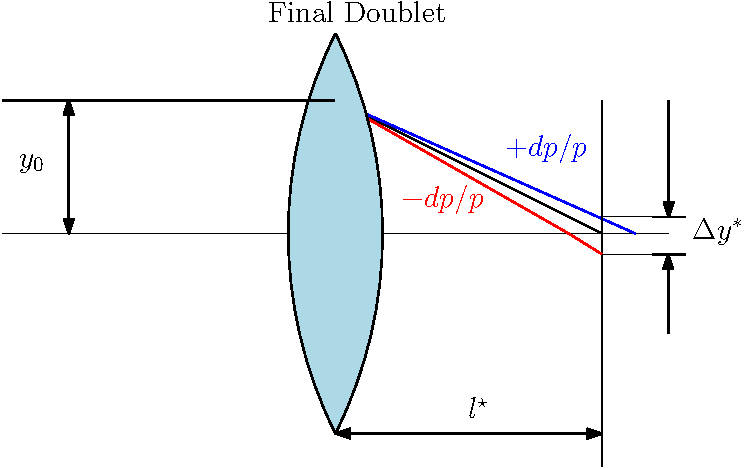
\includegraphics[scale=0.5]{chromaticity.pdf}\caption{Chromaticity.}\label{f:chrom}
\end{figure}
\subsection{Tuning}
When considering imperfections, the machine performance decreases dramatically, typically, the beam size increases and luminosity drops substantially about 6 orders of magnitud. The tuning is the procedure which brings the system performance to its design values. Since the initial errors are unknown, the tuning requires a statistical study. Usually more than 100 machines with randomly distributed errors are considered in computer simulations. The simulated tuning reproduces a realistic tuning procedure in a machine \cite{GarciaMorales:1982827,Minty:629879}.\par

\chapter{Current Linear Collider Projects}\label{s:lincoll}

\section{Compact Linear Collider (CLIC)}
The CLIC \cite{CLICdes} is designed to collide electrons and positrons at 3~TeV c.o.m. with total luminosity of $6\times10^{34}$~cm$^{-2}$s$^{-1}$. The innovative proposal of two-beam acceleration is explored to accomplish the high accelating gradient of the order of 100~MV/m. The RF power is extracted from a low-energy and high-intensity beam, the drive beam, and fed into the main beam via Power Extraction and Transfer Structures (PETS). This concept reduces the length of the accelerating system compared to superconducting technology.\par
The CLIC studies were initially concentrated in 3~TeV, with a 500~GeV stage. Table~\ref{t:CLICparam} shows the main beam parameters and Fig.~\ref{f:CLIClayout} show the 500~GeV and 3~TeV layouts. Recently the CLIC~500~GeV has been reconsidered due to the 125~GeV mass bosson founded by the LHC experiments CMS and ATLAS, concluding a new CLIC stage at 380~GeV c.o.m.\par
The most critical areas for the CLIC design the ability to achieve the 100~MV/m accelerating gradient, the generation, stabilization and deceleration of the drive beam, the ultra-low emittances in the damping rings and their preservation up to the collision point, the ability to protect the machine to damage, and the beam size minimization.\par
\begin{table}[h]
 \centering
 \begin{tabular}{l||c|c}\hline
 Parameter, Symbol, [Unit] & CLIC~3TeV & CLIC~500~GeV \\\hline\hline
 Center of mass, $E_{cm}$, [GeV] & 3000 & 500\\
 Repetition rate, $f_{rep}$, [Hz] & 50 & 50\\
 Bunch population, $N_e$  & $3.72\times10^9$ & $6.8\times10^9$\\
 Number of bunches, $n_b$ & 312 & 354 \\
 Bunch separation, $\Delta t_b$, [ns] & 0.5 & 0.5\\
 Accelerating gradient, $G$, [MV/m] & 100 & 80\\
 Bunch length, 	$\sigma_z$, [$\mu$m] & 44 & 72 \\
 IP Beam size, $\sigma_x,\sigma_y$, [nm] & 40/1 & 200/2.26\\
 Normalized beam emittance (IP), $\epsilon_{nx}/\epsilon_{ny}$, [nm] & 600/20 & 2400/25\\
 Total Luminosity, $L_{tot}$, [$10^{34}$cm$^{-2}$s$^{-1}$] & 5.9 & 2.3\\
 Site length, [km] & 48.3 & 13.0\\\hline
 \end{tabular}\caption{CLIC Beam Parameters.}\label{t:CLICparam}
\end{table}
\begin{figure}[h]
\centering
\begin{subfigure}{1.0\textwidth}
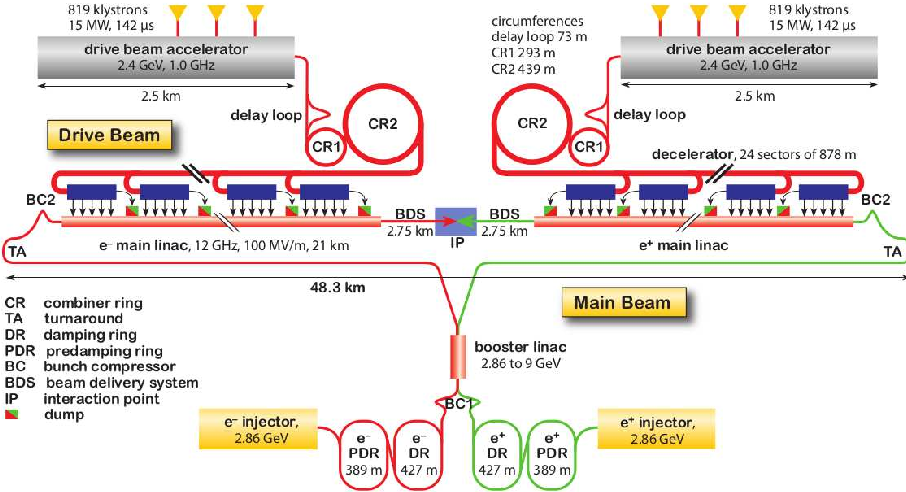
\includegraphics[scale=1.0,angle=0]{CLIC3TeV_layout-crop.pdf}\caption{CLIC~3TeV layout.}\label{f:CLIC3TeVlayout} 
\end{subfigure}\par
\begin{subfigure}{1.0\textwidth}
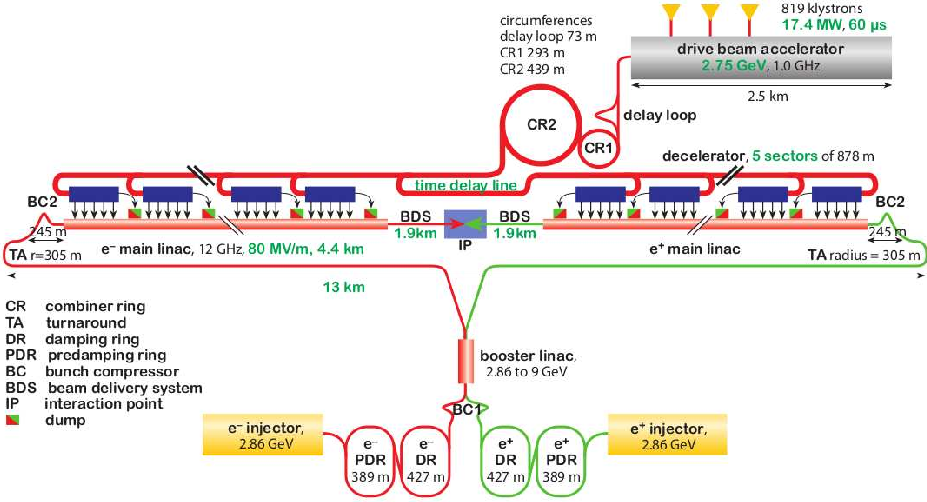
\includegraphics[scale=1.0,angle=0]{CLIC500GeV_layout-crop.pdf}\caption{CLIC~500~GeV layout.}\label{f:CLIC500GeVlayout} 
\end{subfigure}\caption{CLIC~500~GeV FFS.}\label{f:CLIClayout}
\end{figure}
The CLIC~3TeV and 500~GeV FFS has been studied in \cite{GarciaMorales:1982827} with local and non-local chromaticity correction and concluded that the non-local is longer about 1~km longer than the local but only for high energies. At low energies both require a similiar length. Both achieve a similar luminosity, however, the main difference come from tuning simulations where the non-local shows easier tuning at high energies, which translates to larger integrated luminosity and larger statistics for the particle physics analysis. Figure~\ref{f:CLIC3TeVFFS} shows the non-local and local chromaticity correction lattices for 3~TeV and Fig.~\ref{f:CLIC500GeVFFS} for the 500~GeV case.\par
\begin{figure}[h]
\centering
\begin{subfigure}{0.5\textwidth}
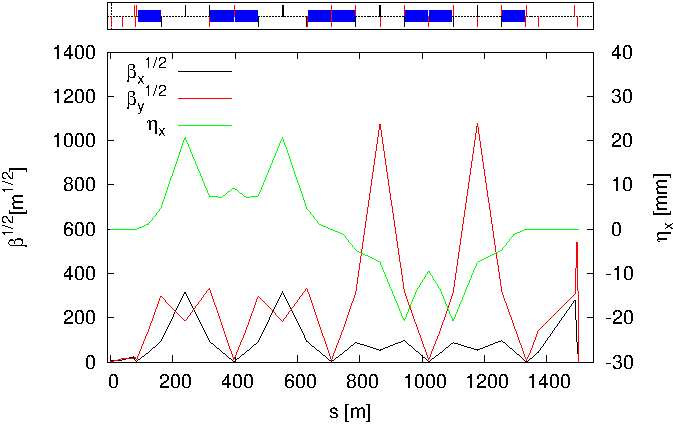
\includegraphics[scale=0.7,angle=0]{CLIC3TeV_FFS_nonlocal-crop-crop.pdf}\caption{Non-local chromaticity correction.}\label{f:CLIC3TeVFFSnonlocal}
\end{subfigure}\hspace*{0.5cm}
\begin{subfigure}{0.5\textwidth}
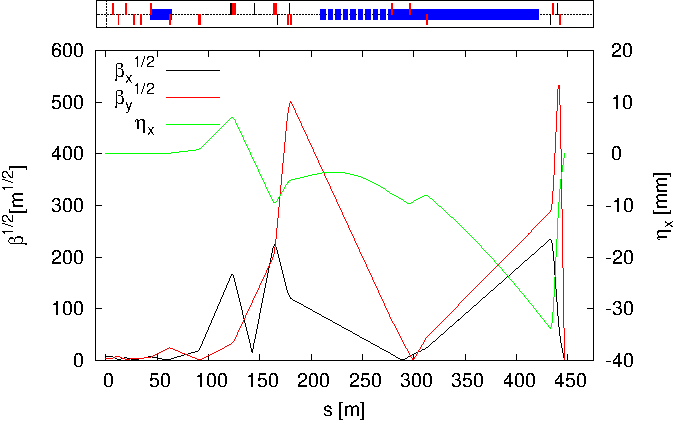
\includegraphics[scale=0.7,angle=0]{CLIC3TeV_FFS_local-crop-crop.pdf}\caption{Local chromaticity correction.}\label{f:CLIC3TeVFFSlocal} 
\end{subfigure}\caption{CLIC~3~TeV FFS.}\label{f:CLIC3TeVFFS}
\end{figure}
\begin{figure}[h]
\centering
\begin{subfigure}{0.5\textwidth}
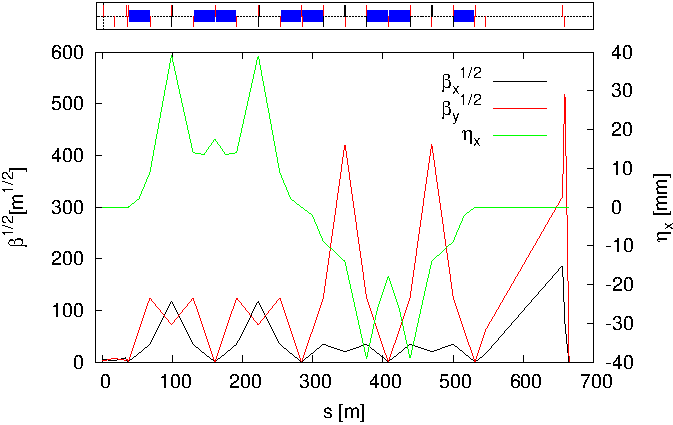
\includegraphics[scale=0.7,angle=0]{CLIC500GeV_FFS_nonlocal-crop-crop.pdf}\caption{Non-local chromaticity correction.}\label{f:CLIC500GeVFFSnonlocal} 
\end{subfigure}\hspace*{0.5cm}
\begin{subfigure}{0.5\textwidth}
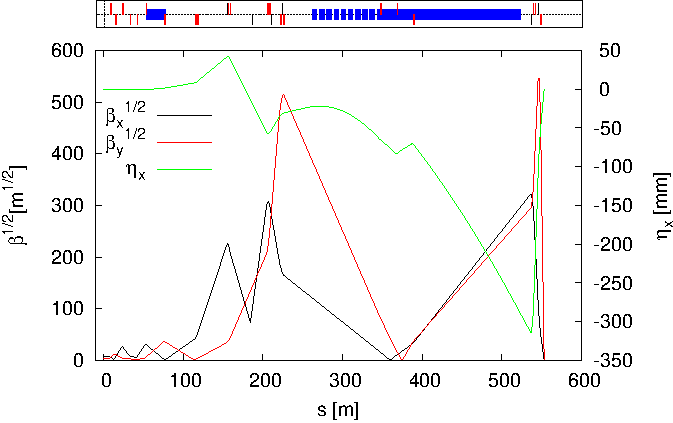
\includegraphics[scale=0.7,angle=0]{CLIC500GeV_FFS_local-crop-crop.pdf}\caption{Local chromaticity correction.}\label{f:CLIC500GeVFFSlocal} 
\end{subfigure}\caption{CLIC~500~GeV FFS.}\label{f:CLIC500GeVFFS}
\end{figure}

\section{International Linear Collider (ILC)}
The ILC \cite{ILCdes} is designed to have a continuous center-of-mass energy range between 200~MeV and 500~GeV, and peak luminosity $L=2\times10^{34}$~cm$^{-2}s^{-1}$, consistent with producing 500~fb$^{-1}$ in the first four years of operation. In adittion, the machine should be upgradable to a center-of-mass of 1~TeV. It has been designed to achieve and energy stability and precision of 0.1~\%, and to have 80\% electron polarization at the IP as well as an option for 60\% positron polarization. Furthermore, alternative options for $\gamma\gamma$ and $e^-e^-$ collisions are under consideration.\par
The main technological challenge in ILC is based in 1.3~GHz superconducting radio frequency accelerating cavities with gradient of 31.5~MV/m each. One other challenge is the beam minimization due to the tight tolerances to obtain nanometer vertical beam size.\par
Figure~\ref{f:ILC} shows the ILC schematic layout and Table~\ref{t:ILCparam} shows the chosen beam parameters for ILC such that each subsystem accomodates a range of beam parameters, resulting in flexible operating parameters that will allow identified problems in one area to be compensated for in another.\par
% \subsection{Beam Parameters}
% The nominal ILC beam Parameters set has been chosen to optimize between known accelerator physics and technology challenges throughout the whole accelerator complex, as beam instability and kicker hardware constraints in the Damping Ring (DR), beam current,beam power and pulse length limitations in the main linac, emittance preservation, and acceptable levels of background and kink instability issues at the IP. The ILC has been designed such that each subsystem accomodates a range of beam parameters, resulting in flexible operating parameters that will allow identified problems in one area to be compensated for in another.
\begin{table}[h]
 \centering
 \begin{tabular}{l||c}\hline
 Parameter, Symbol, [Unit] & ILC \\\hline\hline
 Center of mass, $E_{cm}$, [GeV] & 500\\
 Repetition rate, $f_{rep}$, [Hz] & 5.0\\
 Bunch population, $N_e$  & $20\times10^9$\\
 Number of bunches, $n_b$ & 1312 \\
 Bunch separation, $\Delta t_b$, [ns] & 554\\
 Accelerating gradient, $G$, [MV/m] & 31.5\\
 Bunch length, 	$\sigma_z$, [$\mu$m] & 300\\
 IP Beam size, $\sigma_x,\sigma_y$, [nm] & 474/5.9\\
 Normalized beam emittance (IP), $\epsilon_{nx}/\epsilon_{ny}$, [nm] & 10000/35\\
 Total Luminosity, $L_{tot}$, [$10^{34}$cm$^{-2}$s$^{-1}$] & 1.8\\
 Site length, [km] & 31\\\hline
 \end{tabular}\caption{ILC Beam Parameters.}\label{t:ILCparam}
\end{table}
% \subsection{ILC FFS}
The ILC~FFS is shown in Fig.~\ref{f:ILCFFS}. It follows the local chromaticity correction scheme using sextupoles interleaved with the FD. The dispersion, $\eta_x$, at the IP is zero and its derivative, $\eta'_x=\partial \eta_x /ds$, the angular dispersion is about 0.009. The horizontal and vertical sextupoles are interleaved generating third order geometrical aberrations partially corrected by additional sextupoles in proper phase. The residual higher order aberrations are minimized by octupoles and decapoles. The main difference between the CLIC FFS and the ILC FFS design is the presence of dedicated octupoles for the non-linear handling of the beam tails in ILC.\par
An study of the CLIC FFS for the ILC lattice has been carried out in \cite{GarciaMorales:1982827} by reoptimizing the lattice to the nominal requirements and introducing a traveling waist \cite{Balakin} in ILC to increase the luminosity compensating the hourglass effect.
\begin{figure}[h]
\centering
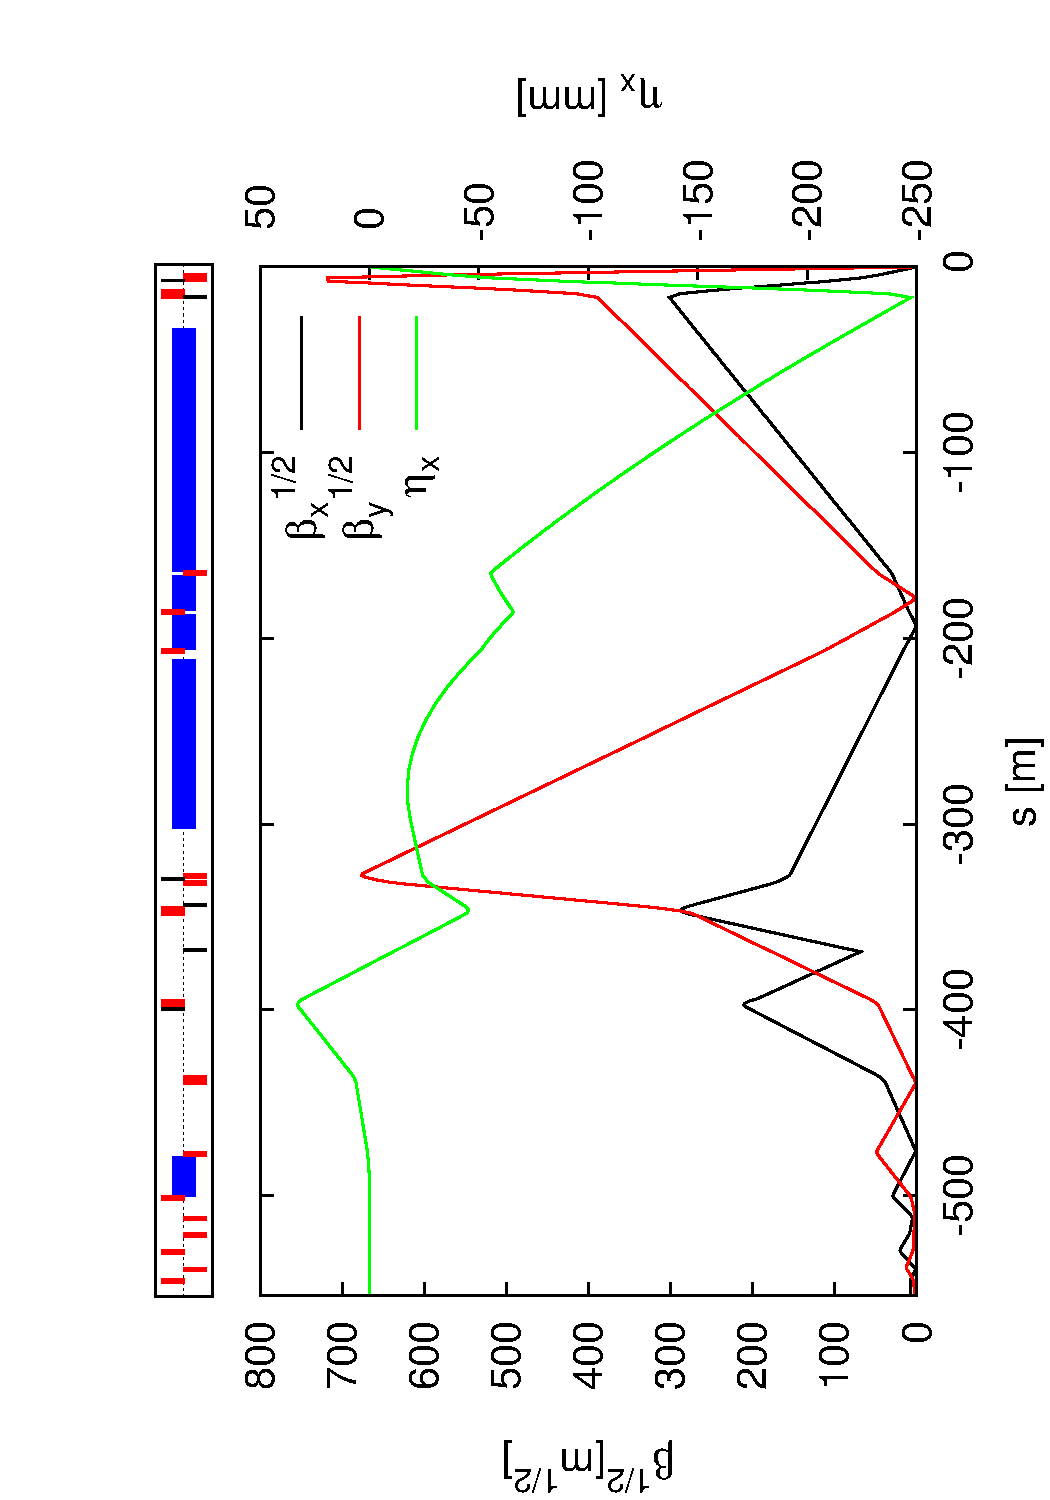
\includegraphics[scale=0.5,angle=-90]{lattice_ILC500_FF.pdf}\caption{ILC~500~GeV~FFS.}\label{f:ILCFFS}
\end{figure}
\begin{figure}[h]
\centering
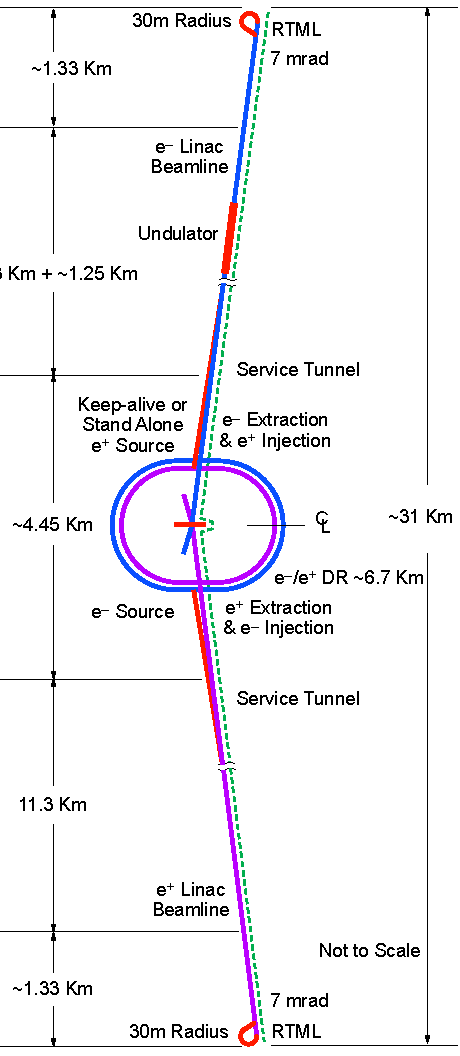
\includegraphics[scale=1.3,angle=0]{ilc.pdf}\caption{ILC schematic layout.}\label{f:ILC}
\end{figure}

\section{Test Facilities}
Several Test Facilities have been constructed for the requred linear colliders R\&D. The following is a brief description of the facility purpose~\cite{GarciaMorales:1982827}.\par
\begin{itemize}
 \item \textbf{CLIC Test Facility 3 (CTF3):} was built at CERN in Geneva, Switzerland, to demonstrate the CLIC two-beam acceleration concept. This requires the high energy accelaration of two beams and the stable decceleration of the drive beam. 
 \item \textbf{Final Focus Test Beam (FFTB):} was built and operated during the 90's at SLAC in California, The United States of America, to reduce the beam size following the non-local chromaticity correction. The smallest vertical beam size measured was 70~nm.
 \item \textbf{Accelerator Test Facility (ATF):} was built at KEK in Tsukuba, Japan, to reduce the beam emittance and vertical  beam size following the local chromaticity correction. The emittance goal has been already achieve and vertical beam sizes down to 44~nm are obtained by systematic tuning of the lattice. This is further explained in Section~\ref{s:ATF2}.
\end{itemize}

%########################################################################
% Second part
%########################################################################
\part{Final focus design for small beam size}
\chapter{Chromaticity in the FFS}\label{s:FFS}
\section{Chromaticity minimization in the Final Doublet (FD)}
% \section{Thin lens approximation}
In this Section I find the Final Doublet distance that minimizes the chromaticity.\par 
In the thin lens approximation, an FD as in Fig.~\ref{f:FDchrom}, with $r=L/L_{IP}$ and $r_{im}=L_{IM}/L_{IP}$, has peak $\beta$-functions at the quadrupoles equal to $\beta_{x0\atop y0}=\frac{L^2_{IP}}{\beta^*_{x\atop y}}$  for $QD0$ and $
\beta_{x1\atop y1}=\beta_{x0\atop y0}\left(1+r\pm\sqrt{\frac{r}{r_{im}}+r+\frac{r^2}{r_{im}}}\sqrt{\frac{1+r}{1+r/r_{im}}}\right)^2
$ for $QF1$, using $\left(\frac{\beta^*}{L_{IP}}\right)^2\ll1$, i.e. a small $\beta$ function far from QD0. The factor $\beta_{x1\atop y1}/\beta_{x0\atop y0}$ is the beta function at QF1 relative to QD0.\par
\begin{figure}[!htb]
 \centering
 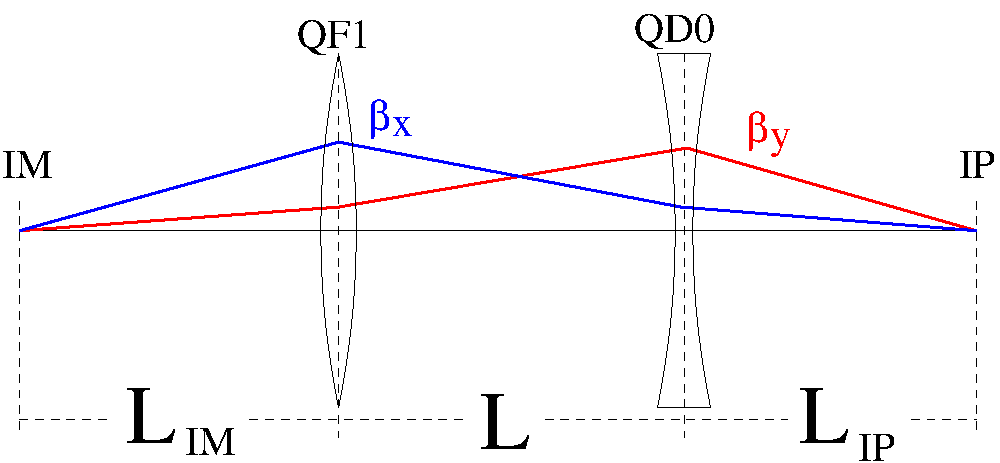
\includegraphics[scale=0.6]{fig01.pdf}\caption{FD with focal points IM and IP at different distances.}\label{f:FDchrom}
 \end{figure}
Being the chromaticity for a single quadrupole as in Eq.~(\ref{eq:chrom}) from~\cite{GarciaMorales:1982827}, 
\begin{equation}
%  \xi_x = \frac{1}{\beta_x^*}\left(\cancelto{0}{T_{116}^2}\beta_{x0}+T_{126}^2\frac{1}{\beta_{x0}}\right)\qquad
%  \xi_y = \frac{1}{\beta_y^*}\left(\cancelto{0}{T_{336}^2}\beta_{y0}+T_{346}^2\frac{1}{\beta_{y0}}\right)\label{eq:chrom}
\xi_{x\atop y}=\int\beta_{x\atop y}(s)k(s)ds\label{eq:chrom}
\end{equation}
where the $k$ is the quadrupole gradient and $s$ the longitudinal coordinate, then, $\xi_{x\atop y}$ can be evaluated as
\begin{equation}
 \xi_{x\atop y}=\mp\left(\beta_{x1\atop y1}k_1l_1-\beta_{x0\atop y0}k_0l_0\right)=\frac{L_{IP}}{\beta^*_{x\atop y}}\Xi_{x\atop y}(r,r_{im})
\end{equation}
where $k,l$ are the quadrupole gradient and length, $\beta^*$ is the $\beta$ function at the IP, the indexes indicate the quadrupole and 
%  \begin{align*}
%  \Xi_{x\atop y}(r,r_{im})=&\mp\sqrt{\frac{1}{rr_{im}}+\frac{1}{r}+\frac{1}{r_{im}}}\sqrt{\frac{1+r/r_{im}}{1+r}}\\ &\left[\left(1+r\pm\sqrt{\frac{r}{r_{im}}+r+\frac{r^2}{r_{im}}}\sqrt{\frac{1+r}{1+r/r_{im}}}\right)^2\right.\\
%  &\qquad\qquad\qquad\qquad\qquad\quad-\left.\left(\frac{1+r}{1+r/r_{im}}\right)\right]
% \end{align*}\par
{\scriptsize
\begin{equation}
 \Xi_{x\atop y}(r,r_{im})=\mp\sqrt{\frac{1}{rr_{im}}+\frac{1}{r}+\frac{1}{r_{im}}}\sqrt{\frac{1+r/r_{im}}{1+r}} \left[\left(1+r\pm\sqrt{\frac{r}{r_{im}}+r+\frac{r^2}{r_{im}}}\sqrt{\frac{1+r}{1+r/r_{im}}}\right)^2\right.-\left.\left(\frac{1+r}{1+r/r_{im}}\right)\right]
\end{equation}}\par
Figure~\ref{f:figT} show the chromaticity $\Xi_x$ and $\Xi_y$ in $L_{IP}/\beta^*$ units, and the ratio of the $\beta$ functions at the quadrupoles.\par
% The IP beam size is increased by chromaticity as $\sigma^*_{x\atop y}=\sigma_{{x0\atop y0}}\sqrt{1+\xi^2_{x\atop y}\sigma_\delta^2}$, where $\sigma_0^2=\beta^*\epsilon$, valid for both transversal planes. Therefore, luminosity is approximately affected by the horizontal and vertical chromaticity as \par
% \begin{equation}
%  L\propto\frac{1}{\sigma_x\sigma_y}=\frac{1}{\sigma_{x0}\sigma_{y0}\sqrt{1+(\xi^2_x+\xi^2_y)\sigma_\delta^2+\xi_x^2\xi_y^2\sigma_\delta^4}}
% \end{equation}
In order to minimize the the product of dispersion and sextupole strengths used to substract the quadrupoles chromatic effect, explained in Section \ref{s:chromcorr}, one possibility is to minimize the sum of the horizontal and vertical chromaticities, i.e. the total chromaticity to be corrected. Being the sum, 
\begin{align}
 \xi = \xi_x + \xi_y &= \frac{L_{IP}}{\beta^*_y}\left(\frac{\Xi_x(r,r_{im})}{\beta^*_x/\beta^*_y}+\Xi_y(r,r_{im})\right)\\
 &= \frac{L_{IP}}{\beta^*_y}\Xi(\beta^*_x/\beta^*_y,r,r_{im})
\end{align}
Figure~\ref{f:fig_3TeV} shows $\Xi$ for CLIC 3 TeV, $\beta^*_x/\beta^*_y=6.9\text{mm}/0.068\text{mm}=101$, and Fig~\ref{f:fig_500GeV} is the equivalent for CLIC 500 GeV \cite{CLICdes}, $\beta^*_x/\beta^*_y=8.0\text{mm}/0.1\text{mm}=80$.\par
Given $L_{IM}$, the minimum added chromaticity in the FD is found when $L$ is one to two times the distance to the IP. In addition, Figs.~\ref{f:fig_3TeV}-\ref{f:fig_500GeV} show the effect of scaling up the system. For example, starting at $L=L_{IP}$ and $L_{IM}=10L_{IP}$, it is clear that a system with $L=10L_{IP}$ and $L_{IM}=100L_{IP}$, will decrease the vertical chromaticity by increasing the horizontal chromaticity.
\begin{figure}
\begin{subfigure}{0.5\textwidth}
 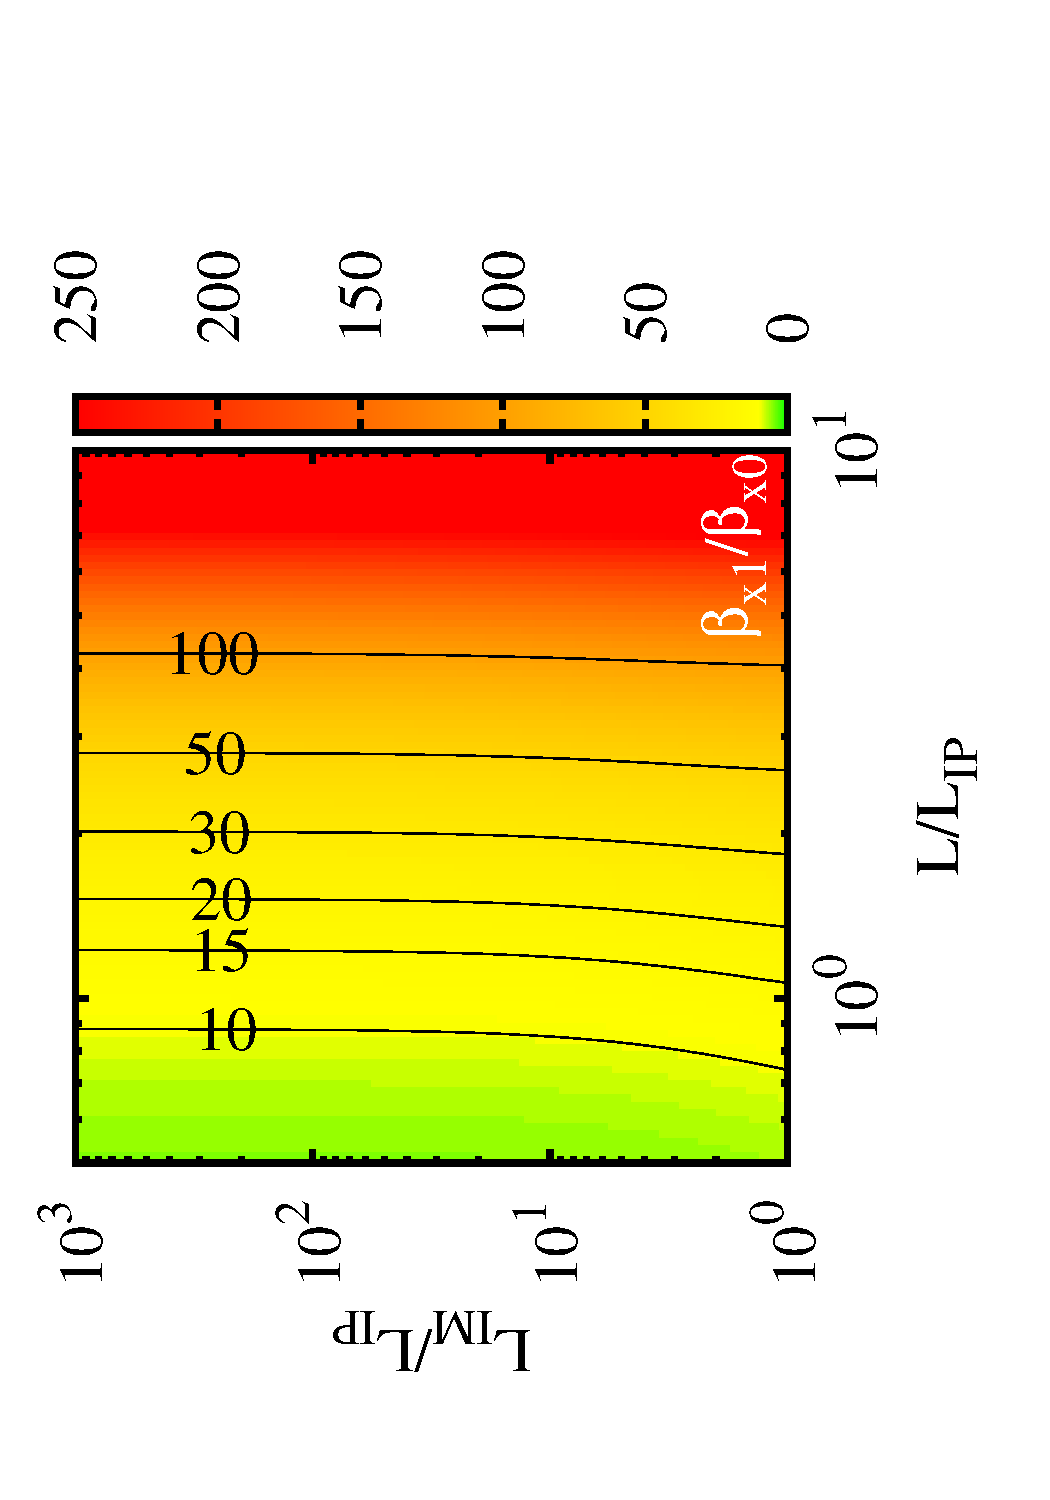
\includegraphics[scale=0.35,angle=-90]{./betax1a.pdf}\caption{}\label{figT:Bx}
 \end{subfigure}
 \begin{subfigure}{0.5\textwidth}
 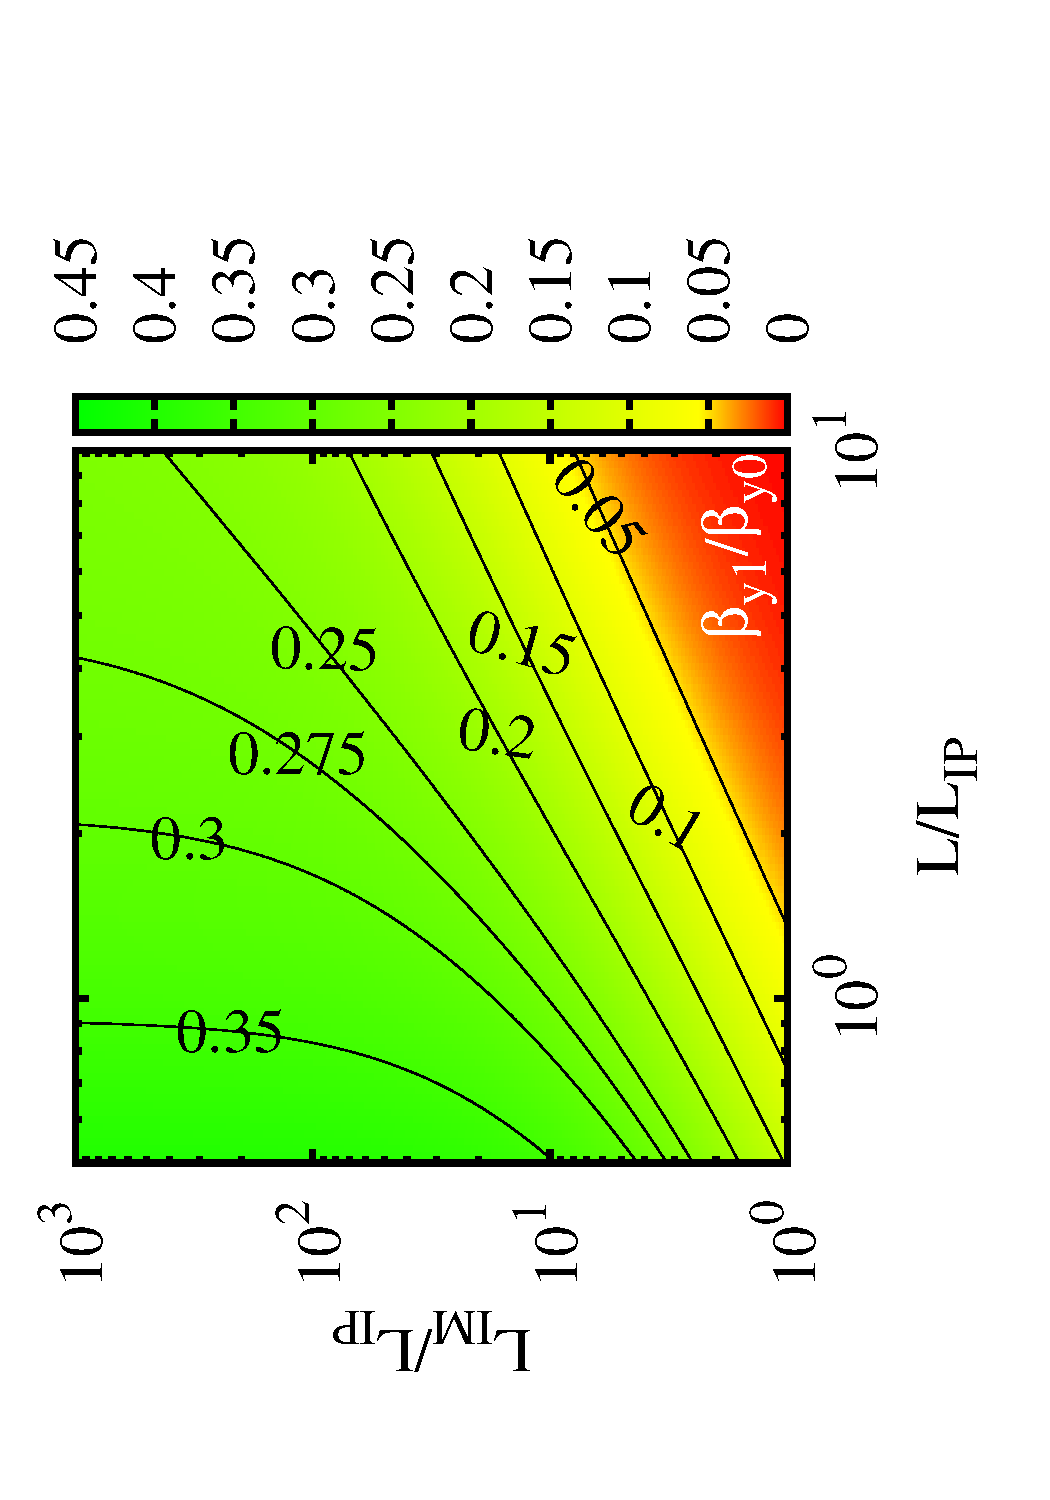
\includegraphics[scale=0.35,angle=-90]{./betay1a.pdf}\caption{}\label{figT:By}
 \end{subfigure}\\
 \begin{subfigure}{0.5\textwidth}
 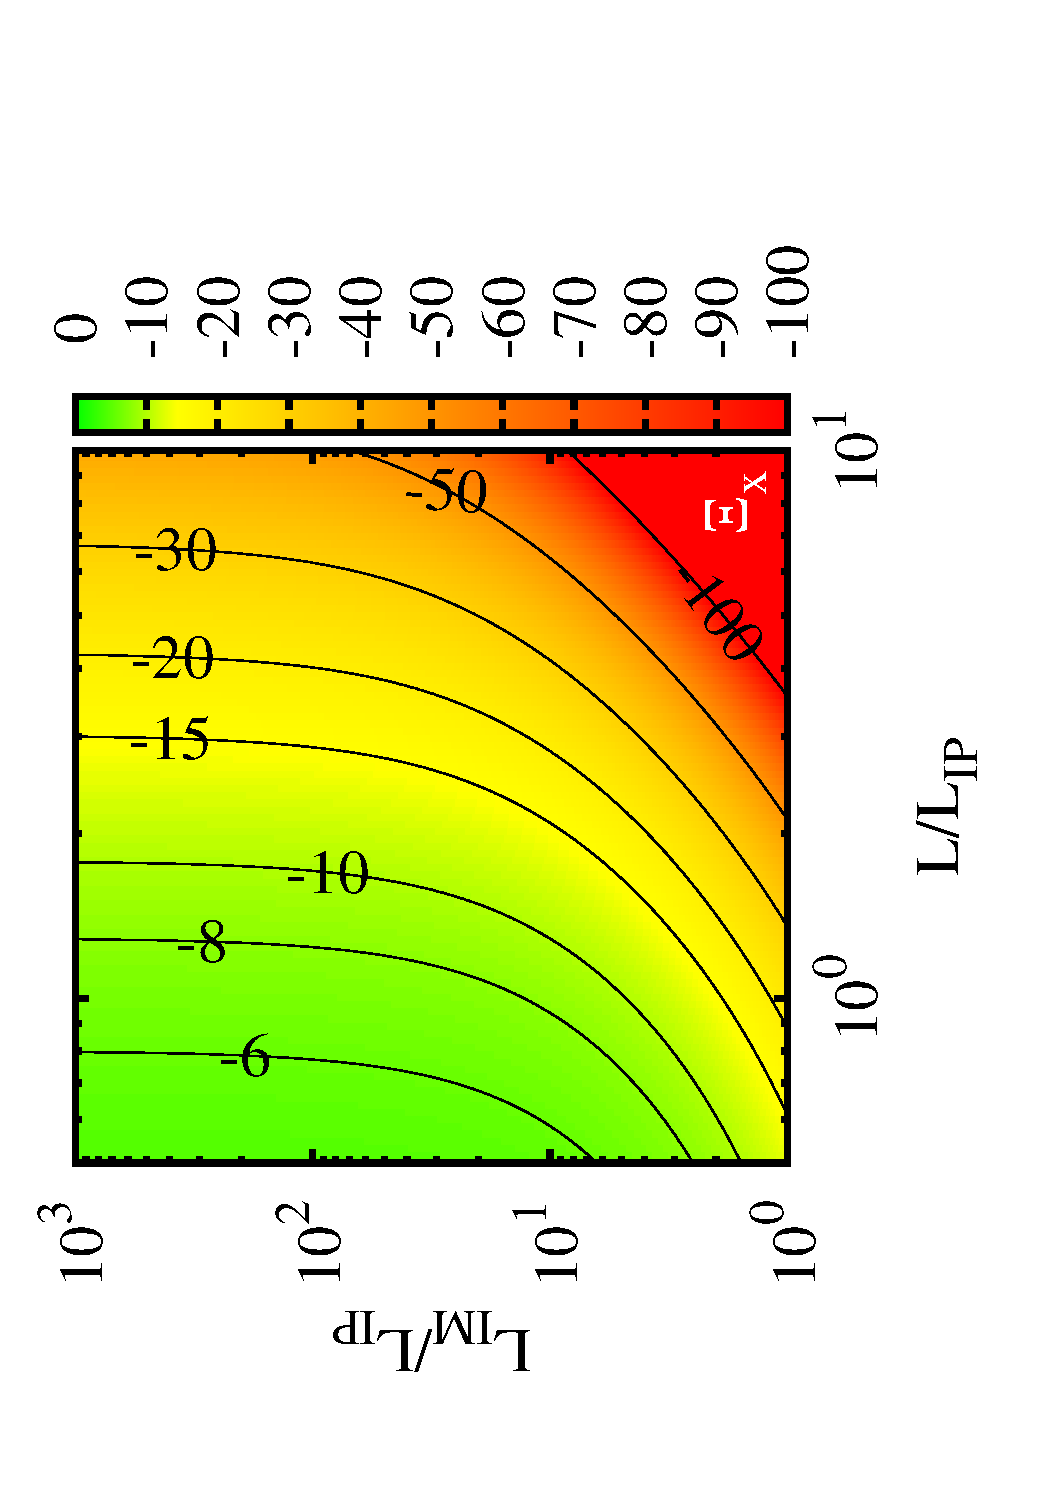
\includegraphics[scale=0.35,angle=-90]{./Xi_xa.pdf}\caption{}\label{figT:xix}
 \end{subfigure}
 \begin{subfigure}{0.5\textwidth}
 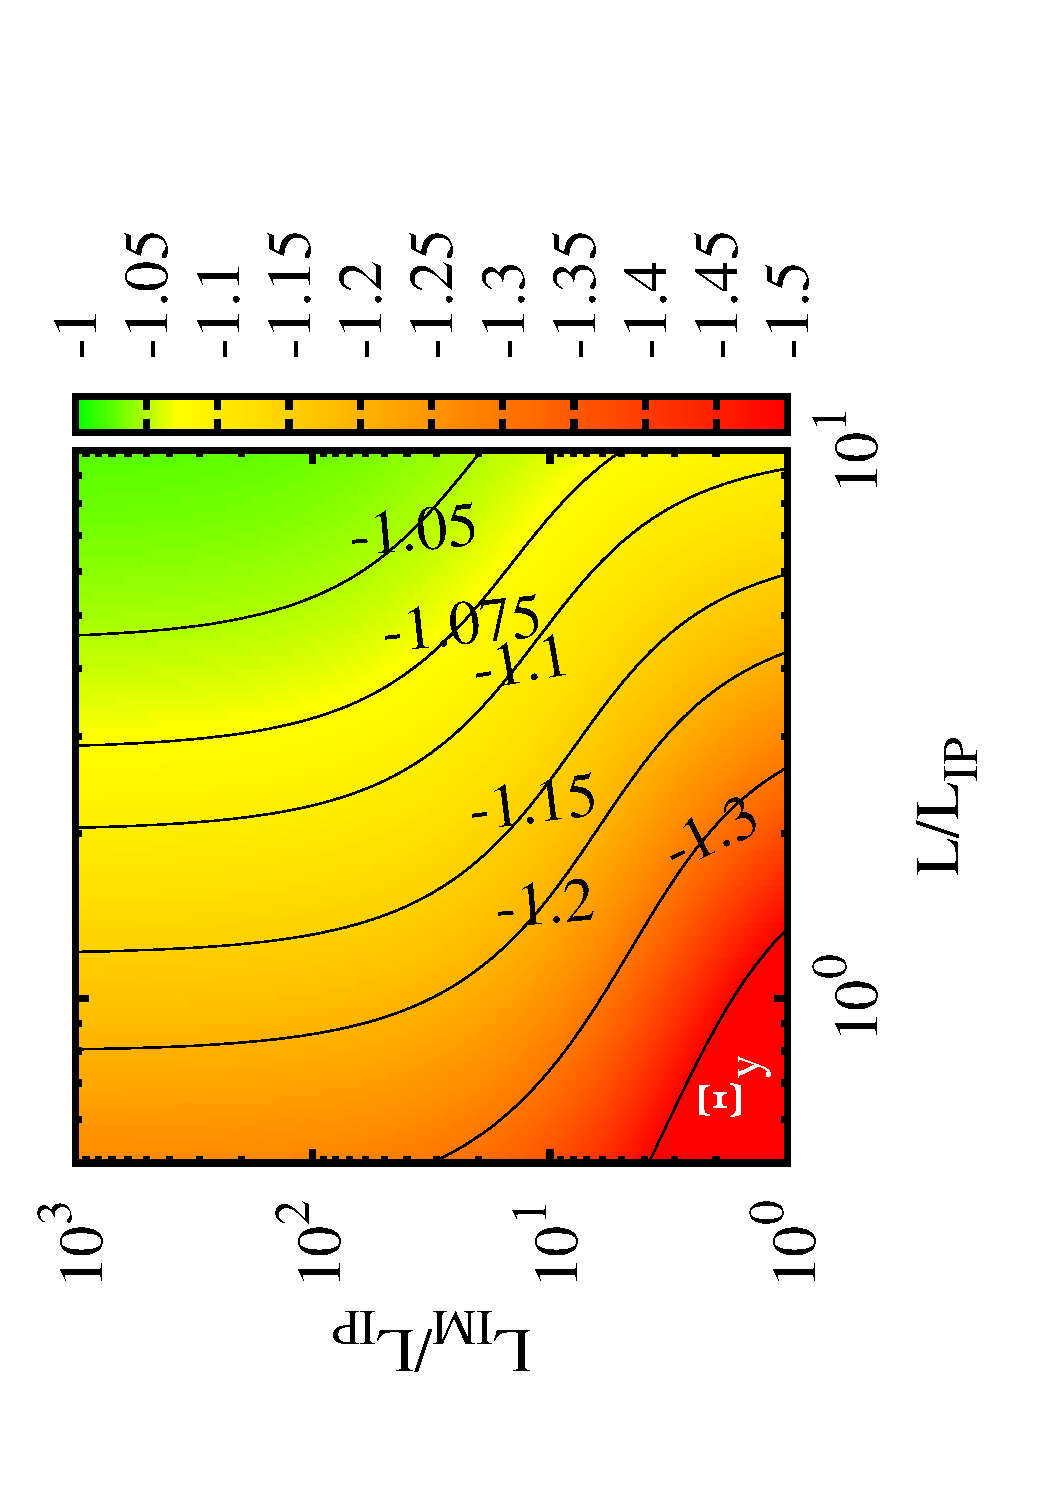
\includegraphics[scale=0.35,angle=-90]{./Xi_ya.pdf}\caption{}\label{figT:xiy}
 \end{subfigure}
 \caption{Normalized transversal functions (\ref{figT:Bx}) $\beta_{x1}/\beta_{x0}$, (\ref{figT:By}) $\beta_{y1}/\beta_{y0}$, (\ref{figT:xix}) $\Xi_x$, (\ref{figT:xiy}) $\Xi_y$}\label{f:figT}
\end{figure}
\begin{figure}
\begin{subfigure}{1.0\textwidth}
 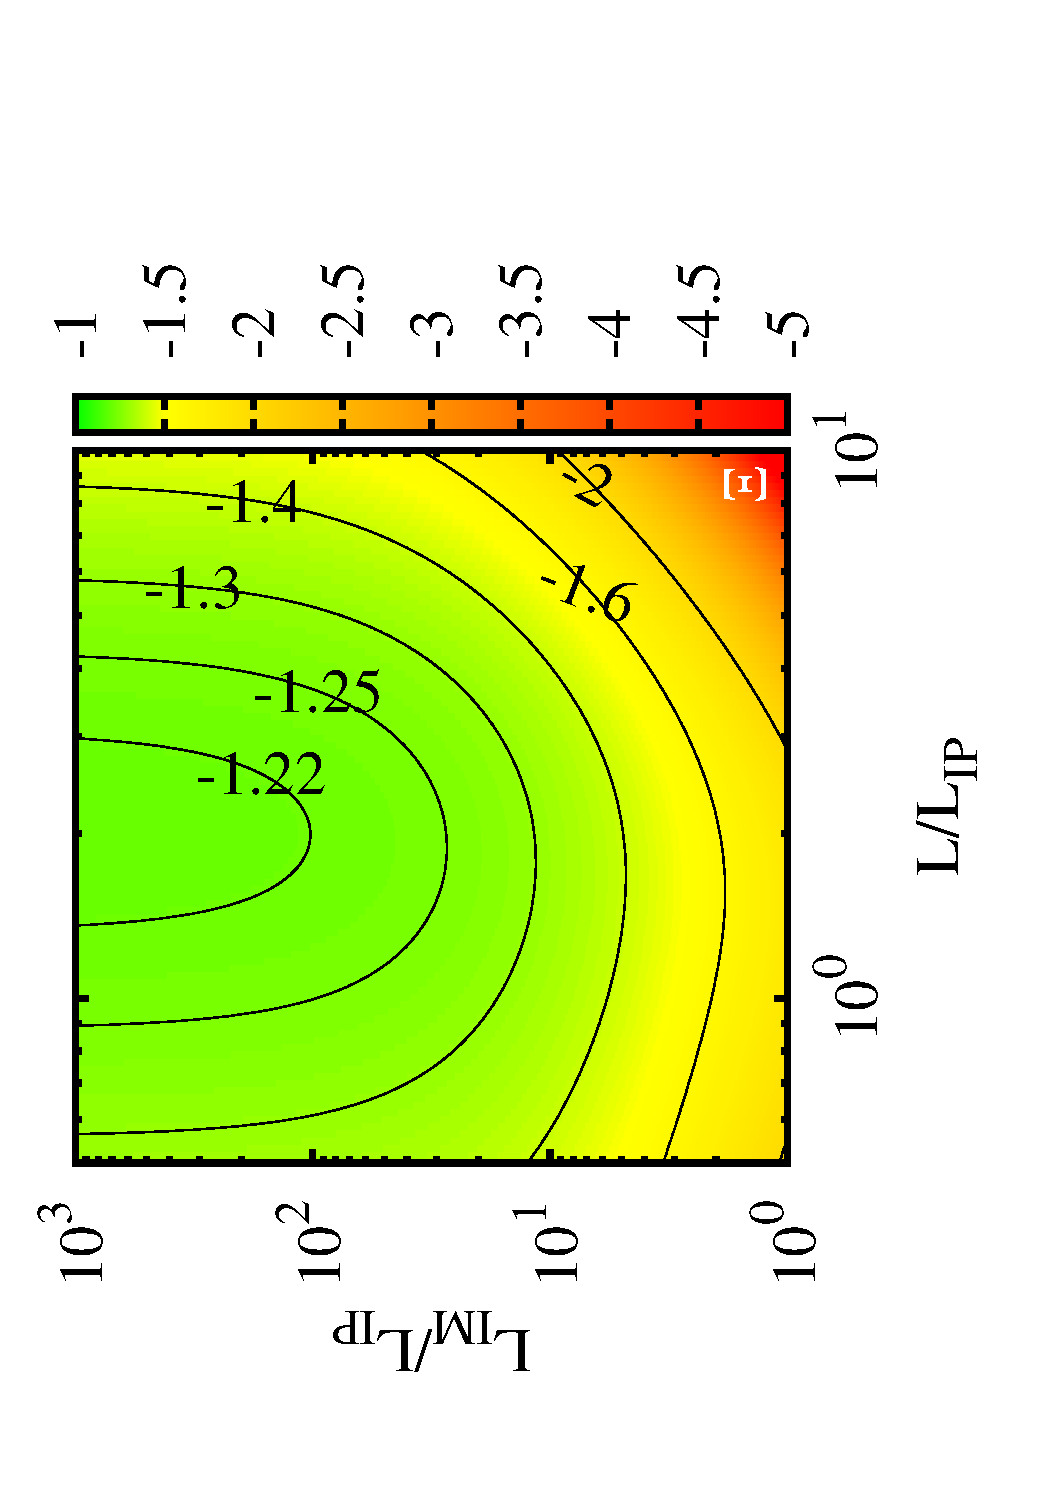
\includegraphics[scale=0.6,angle=-90]{./chromHV_3TeVa.pdf}\caption{}\label{fig_3TeV:chrom}
%  \includegraphics[scale=0.6,angle=-90]{./chromHV_500GeV.pdf}\caption{}\label{fig_chrom:b}
 \end{subfigure}\\
 \begin{subfigure}{0.5\textwidth}
 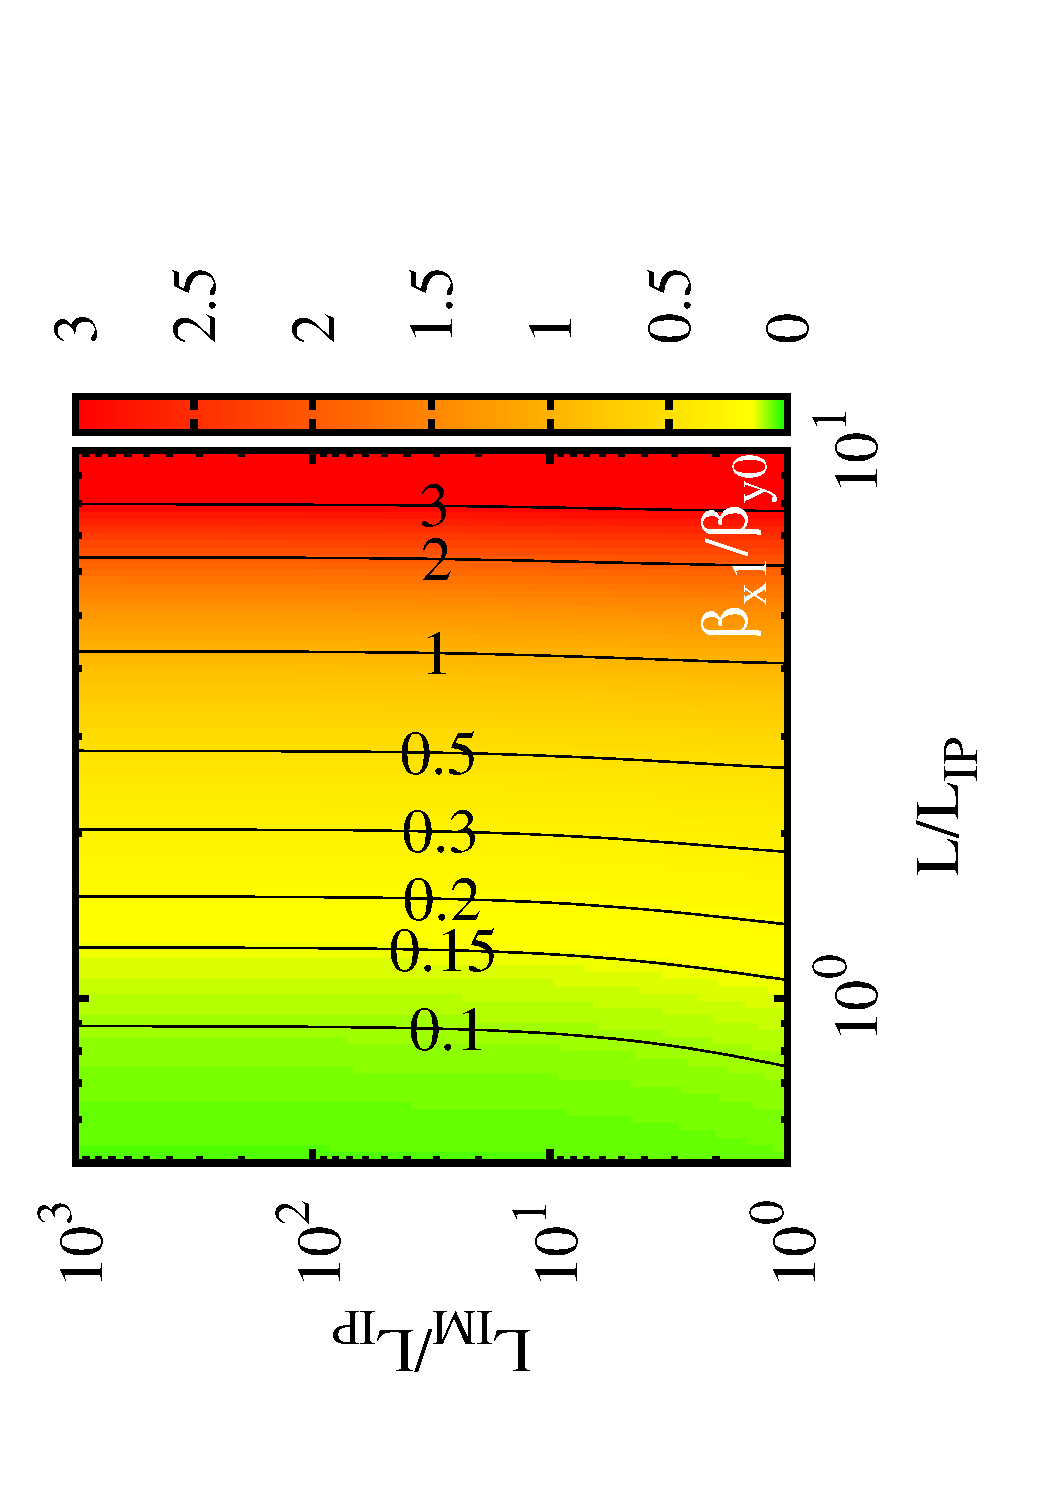
\includegraphics[scale=0.35,angle=-90]{./betax1_y0_3TeVa.pdf}\caption{}\label{fig_3TeV:bx1_y0}
 \end{subfigure}
  \begin{subfigure}{0.5\textwidth}
 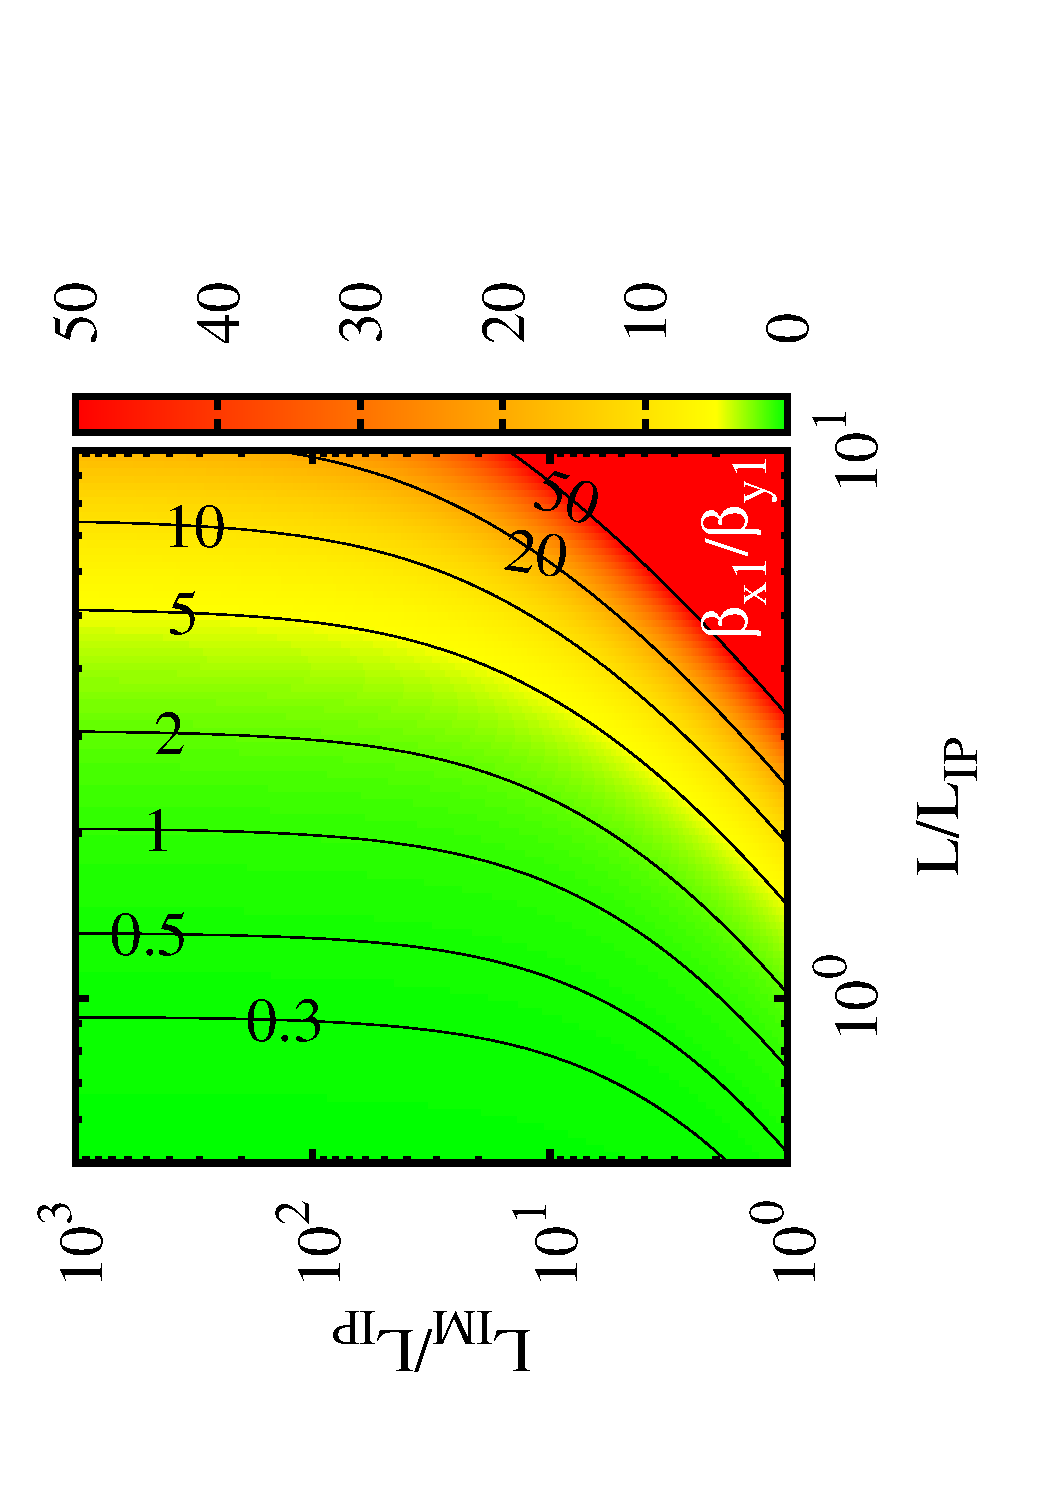
\includegraphics[scale=0.35,angle=-90]{./betax1_y1_3TeVa.pdf}\caption{}\label{fig_3TeV:bx1_y1}
 \end{subfigure}
 \caption{CLIC 3TeV (\ref{fig_3TeV:chrom}) $\Xi(\beta^*_x/\beta^*_y,r,r_{im})$, (\ref{fig_3TeV:bx1_y0}) $\beta_{x1}/\beta_{y0}$, (\ref{fig_3TeV:bx1_y1}) $\beta_{x1}/\beta_{y1}$}\label{f:fig_3TeV}
\end{figure}
\begin{figure}
\begin{subfigure}{1.0\textwidth}
%  \includegraphics[scale=0.6,angle=-90]{./chromHV_3TeV.pdf}\caption{}\label{fig_500GeV:chrom}
 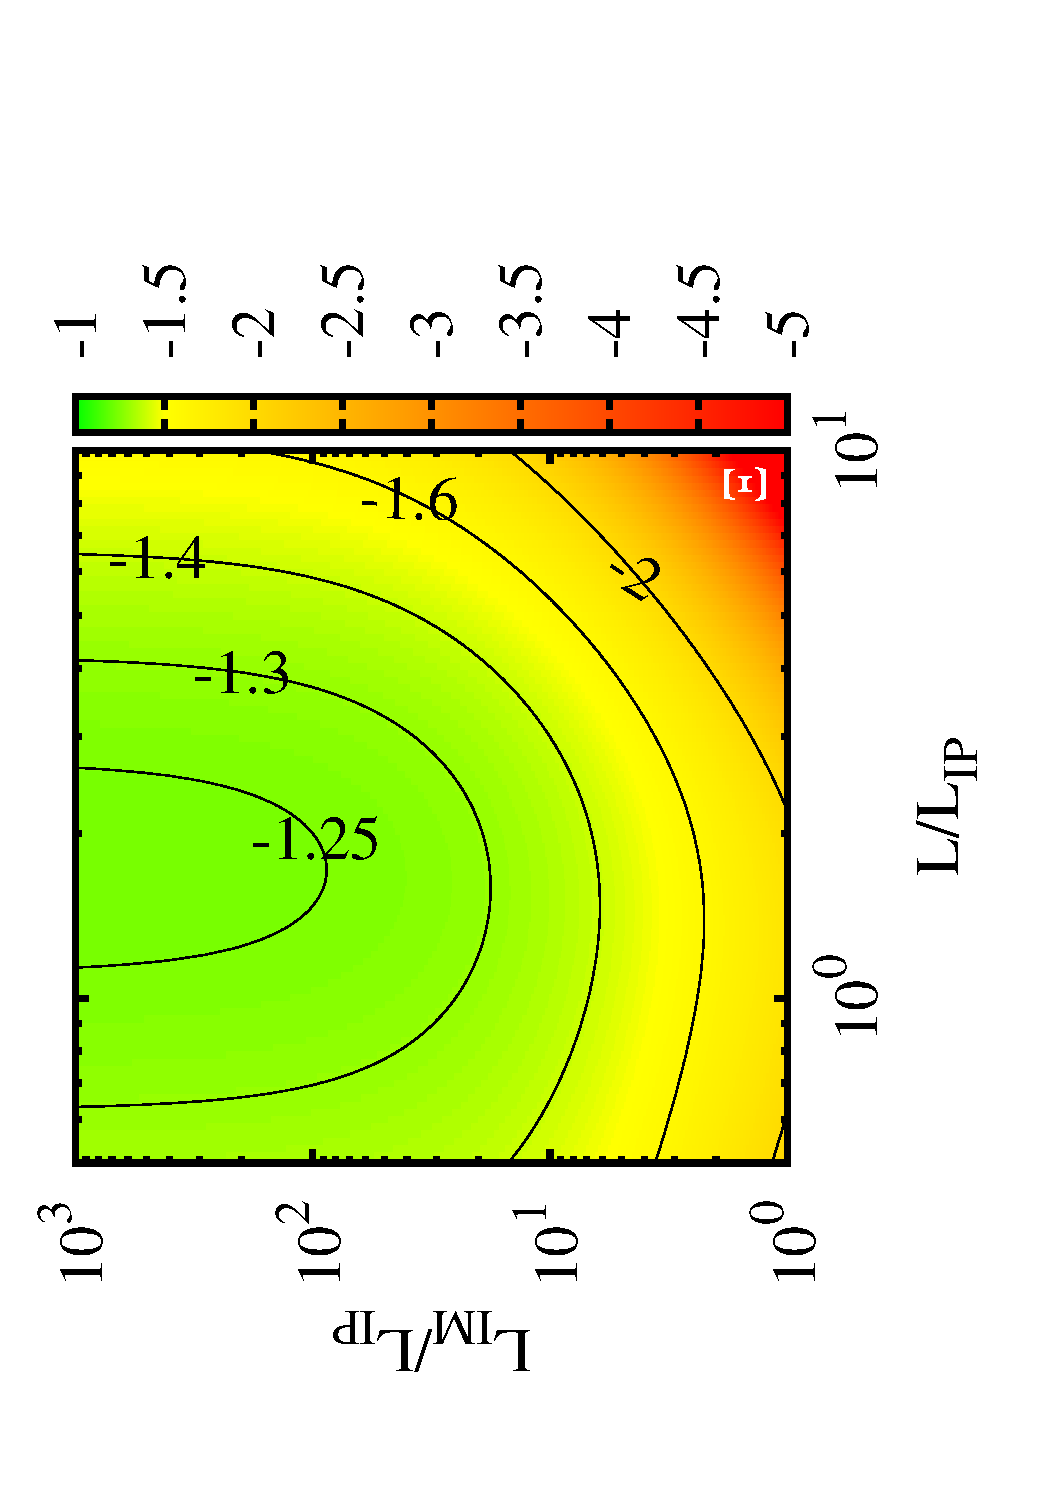
\includegraphics[scale=0.6,angle=-90]{./chromHV_500GeVa.pdf}\caption{}\label{fig_chrom:b}
 \end{subfigure}\\
 \begin{subfigure}{0.5\textwidth}
 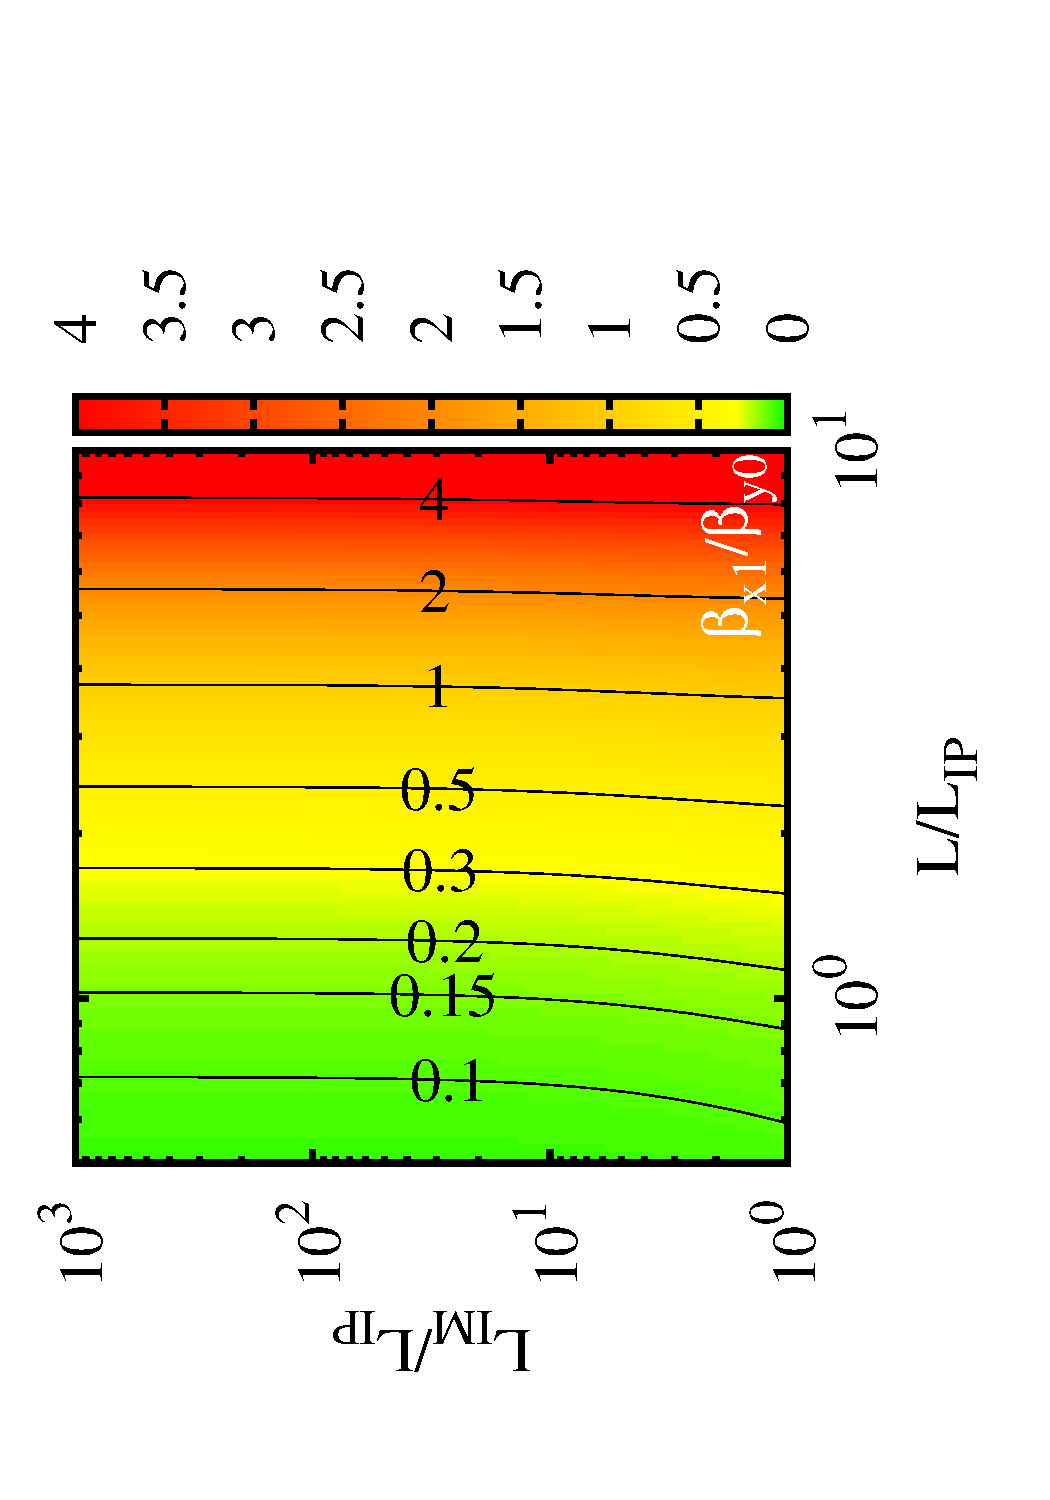
\includegraphics[scale=0.35,angle=-90]{./betax1_y0_500GeVa.pdf}\caption{}\label{fig_500GeV:bx1_y0}
 \end{subfigure}
  \begin{subfigure}{0.5\textwidth}
 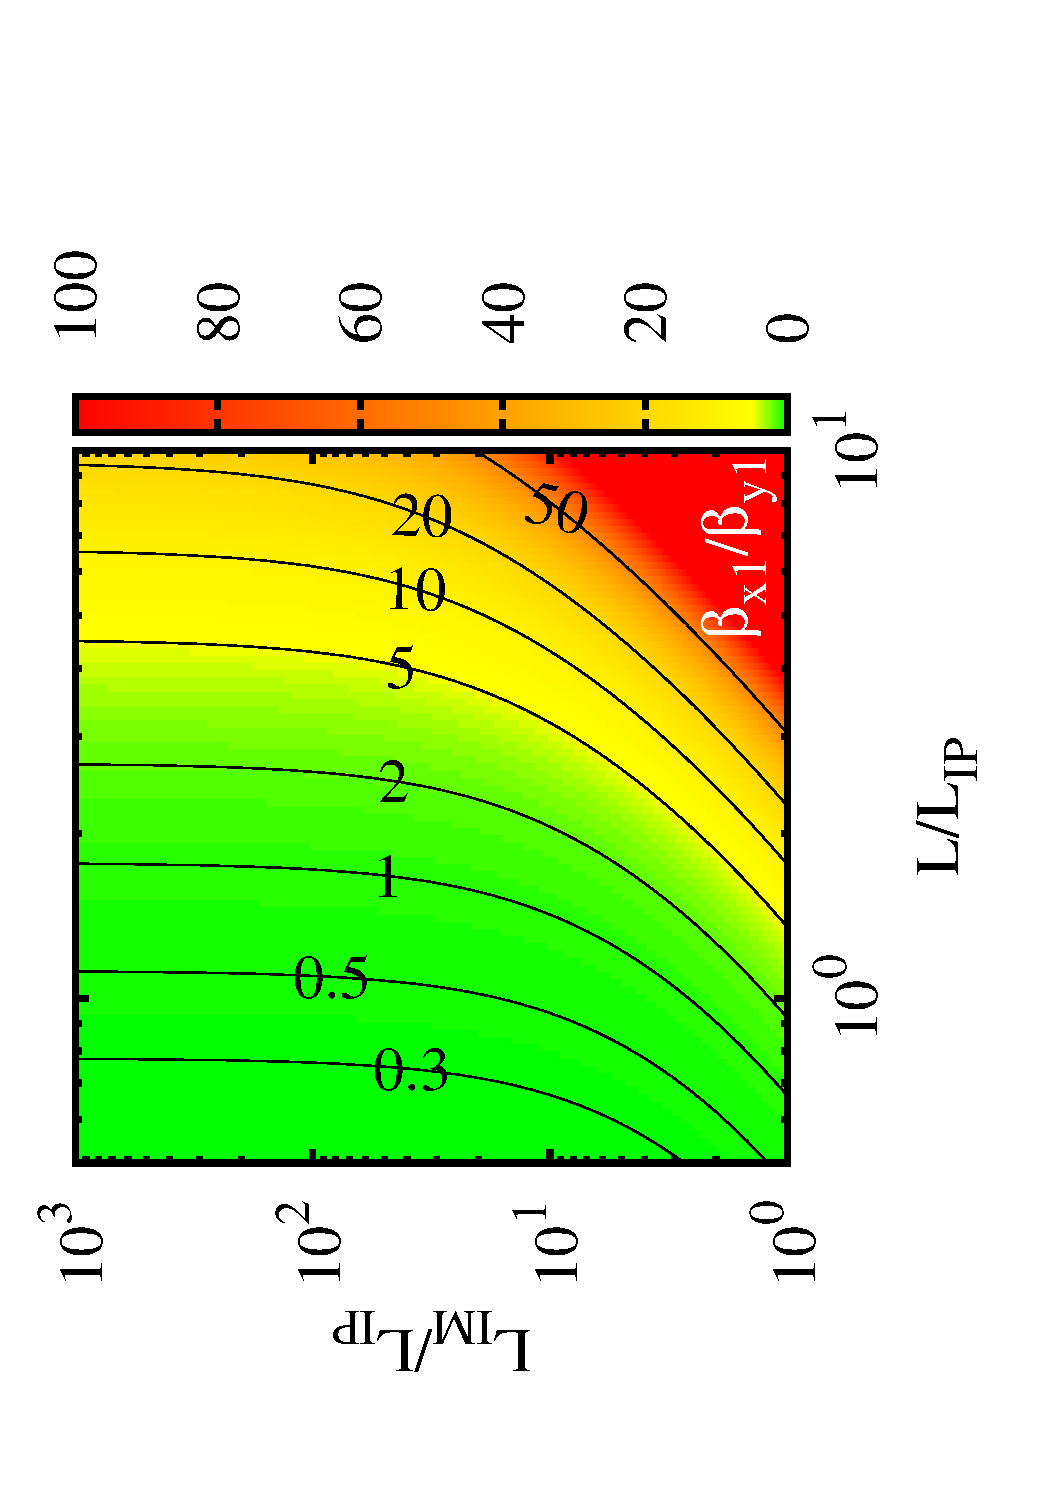
\includegraphics[scale=0.35,angle=-90]{./betax1_y1_500GeVa.pdf}\caption{}\label{fig_500GeV:bx1_y1}
 \end{subfigure}
 \caption{CLIC 500GeV (\ref{fig_3TeV:chrom}) $\Xi(\beta^*_x/\beta^*_y,r,r_{im})$, (\ref{fig_500GeV:bx1_y0}) $\beta_{x1}/\beta_{y0}$, (\ref{fig_500GeV:bx1_y1}) $\beta_{x1}/\beta_{y1}$}\label{f:fig_500GeV}
\end{figure}
\clearpage

\section{The non-interleaved lattice}
\subsection{Introduction}
Large chromaticity is generated in linear colliders due to the ratio of long $L^*$ and low-$\beta^*$ values. Table~\ref{t:chromlat} shows the chromaticity in the current three main linear collider projects.\par
\begin{table}[!htb]
% \scriptsize
\centering
\begin{tabular}{l|c||c|c|c}\hline
Parameter & Symbol & ILC & CLIC 500 GeV& CLIC 3 TeV\\\hline\hline
Distance from IP to QD0 [m] & $L^*$& 3.5/4.5 & 4.3 & 3.5\\
Vertical $\beta$ at the IP [mm] &$\beta_y^*$& 0.48 & 0.1&0.07\\
Energy Spread [$10^{-3}$]& $\delta$&3&3&3\\\hline
Vertical Chromaticity & $\xi_y\approx L^*/\beta^*_y$&7300/9400&43000&50000\\\hline
% Luminosity &$L$& $10^{34}$ &$1.57\times10^{34}$ & $2.3\times10^{34}$&$5.9\times10^{34}$\\\hline
\end{tabular}\caption{Approximative vertical chromaticity for the three current linear collider projects.}\label{t:chromlat}
\end{table}
Two methods have been used to cancel the chromatic effect: non-local and local correction. The local and non-local schemes, presented in Section~\ref{s:chromcorr}, have been compared for CLIC~\cite{PhysRevSTAB.17.101001}, concluding in easier tuning capabilities for the non-local. It has been mainly attributed to the separation of the horizontal and vertical chromatic correction sections, while in the local, the horizontal and vertical correction sections are interleaved.\par
% \subsection{The lattice}
This Section introduces an alternative lattice. In the non-interleaved scheme, the idea is to preserve the separation in the vertical and horizontal chromatic corrections  while cancelling the geometrical components in the vertical plane at the FD. One of the paired sextupoles is inside a horizontally dispersive region while the other remains outside to cancel geometric contributions.\par
\begin{figure}[!htb]
   \centering
   \includegraphics*[scale=0.2,angle=0]{noninterleavedcorr2.pdf}
   \caption{Non-interleaved chromaticity correction.}
   \label{f-noninterleaved}
\end{figure}
 Horizontal dispersion is generated over a common region and it is cancelled upstream, before the FD. Figure~\ref{f-noninterleaved} shows QD0 preceded by a sextupole SD0, which is matched with a second SD1 by the -I transport map. The same configuration is used to cancel horizontal chromaticity in an upstream section of the lattice using SF sextupoles.\par

 \subsection{Geometric Terms Cancellation}
Previously mentioned chromatic correction schemes use a pair of matched sextupoles to cancel one another geometrical components. It is generally noted as the -I transformation. However, results from \cite{PhysRevSTAB.8.104002} show that the -I transformation is one particular solution. When having a pair of sextupoles as in Fig.~\ref{f:sext} joined by a transport matrix $T_{12}$, the general solution is $t_{12}=0$, $t_{34}=0$, $t_{11}t_{22}=1$, $t_{33}t_{44}=1$, $k_{s1}=-k_{s2}t_{11}$ and $t_{11}=\pm t_{33}$, where, $t_{ij}$ are the matrix elements and $k_{s1}, k_{s2}$ are the sextupole gradients. This general solution is used here to give more flexibility to the beta functions in the design. 
\begin{figure}[!htb]
   \centering
   \includegraphics*[scale=0.15,angle=0]{geo_cancel.pdf}
   \caption{Sextupoles joined by the transport matrix $T_{12}$.}
   \label{f:sext}
\end{figure}
Fig. (\ref{f:phaseadv}) shows the relative phase advances required in the non-interleaved design.\par
% \subsection{Tolerances}
Those expressions from the linear transport map set restrictions on the optic lattice parameters and tolerances during the lattice design stage. In order to evaluate those tolerances, $\Delta\phi_x, \Delta\phi_y, r_x, r_y$ have been defined as $\phi_{x12}+\Delta\phi_{x} = \pi$, $\phi_{y12}+\Delta\phi_{y} = \pi$, $ k_{s1}\beta_{x1}^{3/2}-k_{s2}\beta_{x2}^{3/2}+r_x=0$ and $k_{s1}\beta_{y1}^{3/2}-k_{s2}\beta_{y2}^{3/2}+r_y=0$ respectively, where $\Delta\phi$ is the phase advance error, $r$ is the residual after subtractions and $\phi,\beta$ are the optical parameters in horizontal $x$ and vertical $y$ planes for both sextupoles $S1$ or $S2$.\par
\begin{figure}[!htb]
   \centering
   \includegraphics*[scale=0.15,angle=0]{phase_adv.pdf}
   \caption{Phase advance in the non-interleaved lattice design.}\label{f:phaseadv}
\end{figure}
Factors $\alpha_{x1}\Delta\phi_x$, $\alpha_{x2}\Delta\phi_x$, $\alpha_{y1}\Delta\phi_y$, $\alpha_{y2}\Delta\phi_y\ll1$, with $\alpha$ the optic parameter, are conditions to achieve geometrical terms cancellation. The FD requires phase advances finely matched because $\alpha$ and $\beta$ are high, and the residuals $r_x,r_y$ should be close to zero in order to cancel the second order map components in both planes at the same time. The $\beta_y/\beta_x$ ratio can be chosen to match sextupole strengths.\par

\subsection{The Lattice}
Using the CLIC 500 GeV parameters listed in \ref{t:CLIC500GeVnoninterleaved}, new lattices were designed in MAD-X \cite{MADX} following the previous considerations and those in \cite{Seryi-Raimondi2}. Fig. (\ref{f:MAD-X}) is an example. Phase advances have been matched to $10^{-6}$ precision due to high $\alpha$ values in the FD. MAPCLASS2 \cite{Mapclassorig,Mapclass,Mapclass2,githubMapClass2} gives vertical beam size of 1.9nm and horizontal beam size of 186nm to the first order.\par
\begin{table}[!htb]
\centering
 \begin{tabular}{|l|c|}\hline
  \textbf{Parameter [Units]} & \textbf{Value}\\\hline
%   Length (linac exit to IP distance/side [m]) & 1750\\
  Maximum energy/beam [TeV] & 0.25\\
  Distance from IP to first quad, $L^*$ [m] & 4.3\\
%   Crossing angle at the IP [mrad] & 18.6\\
  Nominal core beam size at IP, $\sigma^*$, $x/y$ [nm] & 202/2.3\\
%   Nominal beam divergence at IP, $\theta^*$, $x/y$ [$\mu$rad] & 25/23\\
  Nominal beta-function at IP, $\beta^*$, $x/y$ [mm] & 8/0.1\\\hline
%   Nominal bunch length, $\sigma_z$ [$\mu$m] & 72\\
%   Nominal disruption parameters, $D$, $x/y$ & 0.1/12\\
%   Nominal bunch population, $N$ & $6.8\times10^9$\\
%   Beam power in each beam [MW] & 4.9\\
%   Preferred entrance train to train jitter [$\sigma$] & $<0.2$\\
%   Typical nominal collimation aperture, $x/y$ [$\sigma_x/\sigma_y$] & 10/55\\
%   Vacuum pressure level, near/far from IP [$10^{-9}$ mbar] & 100/10\\\hline
 \end{tabular}\caption{CLIC 500 GeV parameters used for the non-interleaved lattice design.}\label{t:CLIC500GeVnoninterleaved}
\end{table}
\begin{figure}[!htb]
   \centering
   \hspace*{-0.6cm}
   \includegraphics*[scale=0.50,angle=0]{lattice_CLIC500_FF.pdf}
   \caption{Non-interleaved lattice design for CLIC 500 GeV. Dipoles in blue, horizontally focusing quadrupoles in red and above the axis, vertically focusing quadrupoles in red and below the axis, and sextupoles in black.}
   \label{f:MAD-X}
\end{figure}
However, Fig. (\ref{f-beamsize}) shows that the horizontal beam size increases slightly to second order and by more than an order of magnitude when third order components in the map are considered.\par
\begin{figure}[!htb]
   \centering
   \hspace*{-0.6cm}
   \includegraphics*[scale=0.34,angle=0]{sigmas.pdf}
   \caption{Beam size at the IP of the CLIC 500 GeV non-interleaved design as a function of transfer map order obtained with MAD-X PTC.}
   \label{f-beamsize}
\end{figure}
The reason to this beam size growth is the second order dispersion ($T_{166}$) in the sextupole inside the FD, see Fig. (\ref{f-latticeT166}). As opposed to the local chromaticity method were $T_{166}$ is cancelled only at the IP by matching the sextupoles and dispersion function, here, the second order dispersion generates higher order components due to the sextupole inside the FD used for geometrical cancellation. This is not present in the non-local method because there is no sextupole in the FD.\par
Two possible solutions are foreseen at the moment : cancel the map components $T_{166}$ and $T_{266}$ before the FD, or alternatively tolerate some dispersion in the FD to cancel the second order map and making it similar to the local method.\par
\begin{figure}[!htb]
   \centering
   \hspace*{-0.6cm}
   \includegraphics*[scale=0.50,angle=0]{lattice_CLIC500_FF_T166.pdf}
   \caption{CLIC 500 GeV non-interleaved lattice. The second order dispersion from the $T_{166}$ map component is not zero at the sextupole in the FD.}
   \label{f-latticeT166}
\end{figure}
 
 \subsection{Conclusion}
The non-interleaved lattice proposal has been conceived as an alternative to the local and non-local chromaticity correction methods. The added horizontal and vertical chromaticity has been minimized by using a distance from QD0 to QF1 approximately one and two times the distance between QD0 and the IP. Also, a general geometrical cancellation has been used to give more flexibility to the linear lattice design, however the large beta functions close to the FD impose high precision in the phase advance betweeen sextupole elements.\par
The non-interleaved design for CLIC 500 GeV has been diagnosed using MAD-X and MAPCLASS2, concluding that the second order dispersion must be cancelled before the FD because of the high gradient sextupole before QD0 used to cancel geometrical components only.\par
Two solutions are foreseen : the cancellation of the second order dispersion and its derivative before the FD, or alternatively generate dispersion in the FD to cancel the residual second and third order components making it similar to the local correction.\par
Cancellation could be achieved by introducing an additional horizontal focal point upstream with no dispersion and no sextupole, this will increase the amount of total horizontal chromaticity, thereby changing the SF2 and SF3 sextupole strengths without changing the quads in the dispersive region, and enabling perhaps a better cancellation of T166 generated by the quad and sextupole in the dispersive part.% Playing with the magnitudes of the $\beta_x$ peaks at SF3 and SF2 will also change the amount of chromaticity to be corrected, but will not be efficient to improve the cancellation, as both terms (from the quads and SF2) will vary together.

\chapter{Radiation in Bending Magnets}\label{bendrad}
Radiation effects are crucial during the design stage of the lattices, where effects can be evaluated by tracking particles through the lattice or by analytical approximations. However, during the design process this effect is measured at the end, when the optic parameters characterizing the lattice are set. In order to include both, radiation and optic parameters, during the design optimization process, radiation in bending magnets is reviewed in this chapter.\par
The theorie developed by Sands in \cite{Sands} will be first rewrited in order to clarify all terms used in the beam size contribution from the radiation model. As the optics parameters vary during the lattice optimization, then, the analytical result is generalized. This is compared for one dipole and one dipole with a drift  with the tracking code PLACET \cite{Placet} and finally the model validity for the FFS design is analyzed.
\section{Theoretical approximation}\label{radtheo}
Assuming a lattice that can be described by transport matrices in the form written in the Eq. (\ref{eq-matrix}), radiation effects can be calculated by the model in  \cite{Sands}.
\begin{equation}
\begin{pmatrix}
x_2\\
x'_2\\
\delta
\end{pmatrix}
=
\begin{pmatrix}
 C(s_1,s_2) & S(s_1,s_2)& R_{16}(s_1,s_2)\\
 C'(s_1,s_2) & S'(s_1,s_2) & R_{26}(s_1,s_2)\\
 0 & 0 &1
\end{pmatrix}
\begin{pmatrix}
x_1\\
x'_1\\
\delta
\end{pmatrix}
\label{eq-matrix}
\end{equation}
Being $\Delta x_i = R_{16}(s_i,s_p) (-u)/E$, the deviation at the observation point $s_p$ due to the $i^{\text{th}}$ photon of energy $u$ radiated at some point $s_i$, and $E$ the beam energy.\par The first rhs term in Eq. (\ref{eq-sumphot}) is the sum over the $N$ photons radiated during the time $T$ for the particle to cross the magnet. $N(T)$ describes the probability distribution of photon emission. As we are interested only in the second order moment, the mean  $x_0=\langle\sum_{i=1}^{N(T)}\Delta x_i\rangle$ is subtracted from the sum, obtaining $\langle x\rangle=0$, $ \sigma_{bend}^2=\langle x^2\rangle$, being $x$ the horizontal transverse displacement from the reference orbit of a particle at the observation point.
\begin{equation}
\sum_{i=1}^{N(T)}\Delta x_i - x_0 = x\label{eq-sumphot}
\end{equation}
The photon emission follows a Poisson distribution as a consequence of the normalized radiation spectrum and photon number spectrum of synchrotron radiation used in \cite{Sands2} Section 5. For any Poisson-like distribution $\sigma_N^2 = \langle N\rangle$. The beam size contribution due to radiation has two components of variability: the spread of $\Delta x_i$ due to the energy emission $u$ and the number of times the emission process occurs $N$\footnote{Using statistics notation, $\sigma_x=V(x)$ and $\langle x\rangle=E(x)$, then, a process with two components of variability has a variance expressed as $V(x)=E(V(x|N))+V(E(x|N))$. The term $(x|N)$ denotes the evaluation of the $x$ variable for a given $N$}. Therefore, it is calculated as in Eq. (\ref{eq-bsize})
\begin{align}
\sigma^2_{bend} &= \langle x^2\rangle - \cancelto{0}{\langle x\rangle^2} = \langle x^2 \rangle\label{eq-bsize}\\
 &= \langle N\rangle \sigma^2_{\Delta x} + \langle \Delta x \rangle ^2 \sigma_N^2\\
 &= \langle N\rangle \langle (\Delta x)^2\rangle -\cancel{\langle N\rangle\langle\Delta x\rangle^2} + \cancel{\langle \Delta x \rangle^2\langle N \rangle}\\
 &=\langle N\rangle \langle (\Delta x)^2\rangle
\end{align}
Where the $i$ sub-index has been removed intentionally because the photon number emission is extracted from a continuous function of $u$ the photon energy and either $T$ or $s/c$, where $c$ is the speed of light.\par 
The rate of emission of photons is calculated as in Eq. (\ref{eq-nu}) where $K_{5/3}$ is the modified Bessel function, $u_c=\frac{3}{2}\frac{\hbar c \gamma^3}{\rho}$ called the critical energy which depends on the relativistic factor $\gamma$, the reduced Planck constant $\hbar$ and the particle trajectory curvature $\rho$, and $P_\gamma=\frac{2cr_emc^2}{3\rho^2}\gamma^4$ is the instantaneous radiated power where $r_e$ is the classical electron radius and $m$ is the electron mass.
\begin{equation}
n(u,s)=\frac{P_\gamma}{u_c^2}\left[\frac{9\sqrt{3}}{8\pi}\int_{u/u_c}^\infty K_{5/3}(\xi) d\xi\right]\label{eq-nu}
\end{equation}
Using $\Delta x(s) = (-u/E) R_{16}(s,s_p)$ the second moment is calculated by integration over the entire space and energies.
\begin{align}
 \sigma_{bend}^2&=\int_0^{T} \int_0^\infty [\Delta x(u,s)]^2 n(u,s)dudT\label{eqDeltaX}\\
 &=\frac{1}{c}\int_0^{s_p} \int_0^\infty \left[\frac{-u}{E}R_{16}(s,s_p)\right]^2 n(u,s)duds\\
\end{align}
Finally, 
\begin{equation}
\sigma^2_{bend}=C_2\int_0^{s_p} \frac{E^5}{\rho^3}R_{16}(s,s_p)^2 ds\label{eq-R16}
\end{equation}
where $C_2=\frac{55}{24\sqrt{3}}\frac{r_e\hbar c}{(mc^2)^6}=4.13\times10^{-11} \text{ m}^2\text{GeV}^{-5}$ is a constant coming from the emission rate integration already derived by Sands.\par
\subsection{Generalization for the optimization process}\label{s:thebeamrad}
During the optimization process it is convenient to rewrite $R_{16}$ using the off-momentum function $\eta$, lattice parameters and Eq. (\ref{eq-matrix}). Measuring from the reference orbit, the kick propagation from $s$ to $s_p$ can be written in terms of the general transport matrix, giving
\begin{align}
\Delta x(s)_{total}=\frac{-u}{E}\eta(s_p) &= \frac{-u}{E} \left[C(s,s_p)\eta(s) + S(s,s_p)\eta'(s) + R_{16}(s,s_p)\right]\\
\eta(s_p) &= \sqrt{\frac{\beta_{s_p}}{\beta_s}}\left[\eta_s\cos\Delta\phi_{s,s_p}+(\alpha_s\eta_s+\beta_s\eta'_s)\sin\Delta\phi_{s,s_p}\right] + R_{16}(s,s_p)\label{eq-disp}
\end{align}
where $\alpha, \beta$ and $\phi$ are the optics parameters and the subscripts indicate the evaluation point. The equations derived by Sands in \cite{Sands} assume $\alpha_{s_p}=0, \eta_{s_p}=0$ and $\eta'_{s_p}=0$, which are not valid during the lattice optimization process. From Eq. (\ref{eq-R16}) and (\ref{eq-disp}) is clear that the contribution to beam size due to radiation now can be calculated as:
\begin{equation}
 \sigma_{bend}^2=C_2 \int_0^{s_p} \frac{E^5_s}{\rho^3_s}\left\{\sqrt{\frac{\beta_{s_p}}{\beta_s}}\left[\eta_s\cos\Delta\phi_{s,s_p}+(\alpha_s\eta_s+\beta_s\eta'_s)\sin\Delta\phi_{s,s_p}\right]-\eta_{s_p}\right\}^2ds\label{eq-radbends}
\end{equation}
Eq. (\ref{eq-radbends}) was included in MapClass2 in order to be used during lattice design and optimization. It is also worth noting that $\eta_{s_p}=0$ agrees with the result obtained by Sands in the ideal case with zero dispersion at the IP. This generalized expression I obtained is compared with theory and tracking results.

\subsection{One dipole and one dipole with a drift}
First, the theoretical calculation has been derived for the case of one sector magnet ($\rho,L,\theta$) and a sector magnet plus a drift ($L_{drift}$). Beam energy loss is negligible compared with beam energy $E$.\par
For a sector magnet, $R_{16}= \rho(1-\cos\theta)$, the radiation effect is calculated as follows
\begin{align}
\sigma_{bend}^2 &= C_2 E^5\int_0^\theta \frac{1}{\rho^3}[\rho(1-\cos(\theta-\chi))]^2\rho d\chi\\
&= C_2E^5\left[\frac{1}{4}(6\theta-8\sin\theta+\sin(2\theta))\right]\label{eqNum}\\
&=C_2E^5\left(\frac{\theta^5}{20}-\frac{\theta^7}{168}+\frac{\theta^9}{2880}-\frac{17\theta^{11}}{1330560}+O(\theta^{13})\right)
\end{align} 
 In the case of a drift after the bending magnet and defining $j=\frac{L_{drift}}{\rho}=\frac{L_{drift}}{L}\theta$
\begin{align}
  \sigma_{bend}^2 =& C_2 \int_0^\theta E^5\left[1-\cos(\theta-\xi)+\frac{L_{drift}}{\rho}\sin(\theta-\xi)\right]^2 d\xi\\
 =& \frac{C_2}{4} E^5 \left[(1-j^2)\sin(2\theta)-8\sin\theta+4j(1-\cos\theta)^2+(6-2j^2)\theta\right]\label{eqNum2}\\
  =& C_2 E^5 \left[\frac{j^2\theta^3}{3}+\frac{j\theta^4}{4}-\frac{(4j^2-3)\theta^5}{60}- \frac{j\theta^6}{24} +\frac{(16j^2-15)\theta^7}{2520}+\frac{j\theta^8}{320}\right.\notag\\
    &-\frac{(64j^2-63)\theta^9}{181440}-\frac{17j\theta^{10}}{120960}+\frac{(256j^2-255)\theta^{11}}{19958400}+\frac{31j\theta^{12}}{7257600}\notag\\
    &\left.-\frac{(1024j^2-1023)\theta^{13}}{3113510400}+O(\theta^{14})\right]
\end{align}
Eqs. (\ref{eqNum}) and (\ref{eqNum2}) will be used to normalize the results from MAPCLASS2 and PLACET \cite{Placet} where some care should be taken due to numerical precision.\par
\section{Comparison of theory and tracking results}\label{s:comparison}
The theoretical result is now compared with the general expression included in MAPCLASS2, Eq. (\ref{eq-radbends}), and the tracking code PLACET in the case of one dipole and one dipole and a drift. This can be seen in Fig. (\ref{figSR}), normalized to the theoretical values in Eqs. (\ref{eqNum}) and (\ref{eqNum2}), where radiation effect in PLACET was obtained by subtracting the squared beam size from two trackings with same input parameters except for radiation ON/OFF.\par
Figures (\ref{figSR}) (a) and (b) show the effect of systematic change of $\theta$ while keeping $\rho$ and $L$. Figures (\ref{figSR}) (c) and (d) show the effect of changing $L$ while keeping $\rho$ and $\theta$. Figures (\ref{figSR}) (e) and (f) show the effect of changing $L_{drift}$ while keeping the magnet constant. The equivalent magnetic field $B$ is calculated using the magnetic rigidity $B\rho=P/e$ for $E=1.5 $ TeV.\par
When observing the PLACET results, the left side of the plot shows an agreement of (80$\sim$90)\% between the theoretical value and the tracking, while the right side shows perfect agreement in almost all cases. The difference is the tracking method used by PLACET.\par
In PLACET 0.99.01 two different implementations of radiation exist: the first one will be called `default' and the second `six\_dim'. `Default' calculates radiation by segmenting the dipole in a \emph{default} number of shorter pieces with Binomial probability of photon emission when the particle traverses each slide. This is called thin dipole approximation and it is also the default tracking method. On the other side, `six\_dim' does not make any sectioning of the dipole, it uses the Poisson probability of photon emission over the entire  dipole, as in the theory.\par
This was confirmed with several variations of the code provided by the authors of PLACET where the number of slices were increased, making the Binomial probability to approach the Poisson results.\par
As expected, the MAPCLASS2 and the theoretical results are in good agreement, showing the validity of the generalization in Sect. \ref{s:thebeamrad}. Only Figs. (a) and (b) show abrupt changes at $\theta=7.5\times10^{-7}$ rad due to Twiss result from `ptc\_twiss' 5 dim in MAD-X \cite{MADX}. It is however for very small angles and magnetic fields where a recalculation of the optic parameters using the `twiss' function in MAD-X showed no abrupt changes.\par
There is a point to highlight using Fig. (\ref{figSR}) (b). The tracking, theorical and general calculations are all in good agreement in the range of angles between $10^{-2}$ and $10^{-5}$ rad. Below $10^{-5}$ rad the agreement again decays to (80$\sim$90)\%. It is related to the average number of photons emitted when traversing the dipole and it is explored in Sect \ref{s:modellim}.\par
\begin{figure}[htb]
\centering
  \hspace*{1.2cm}`Default' Synrad\hspace*{5.0cm}Flag `-six\_dim 1'\par
 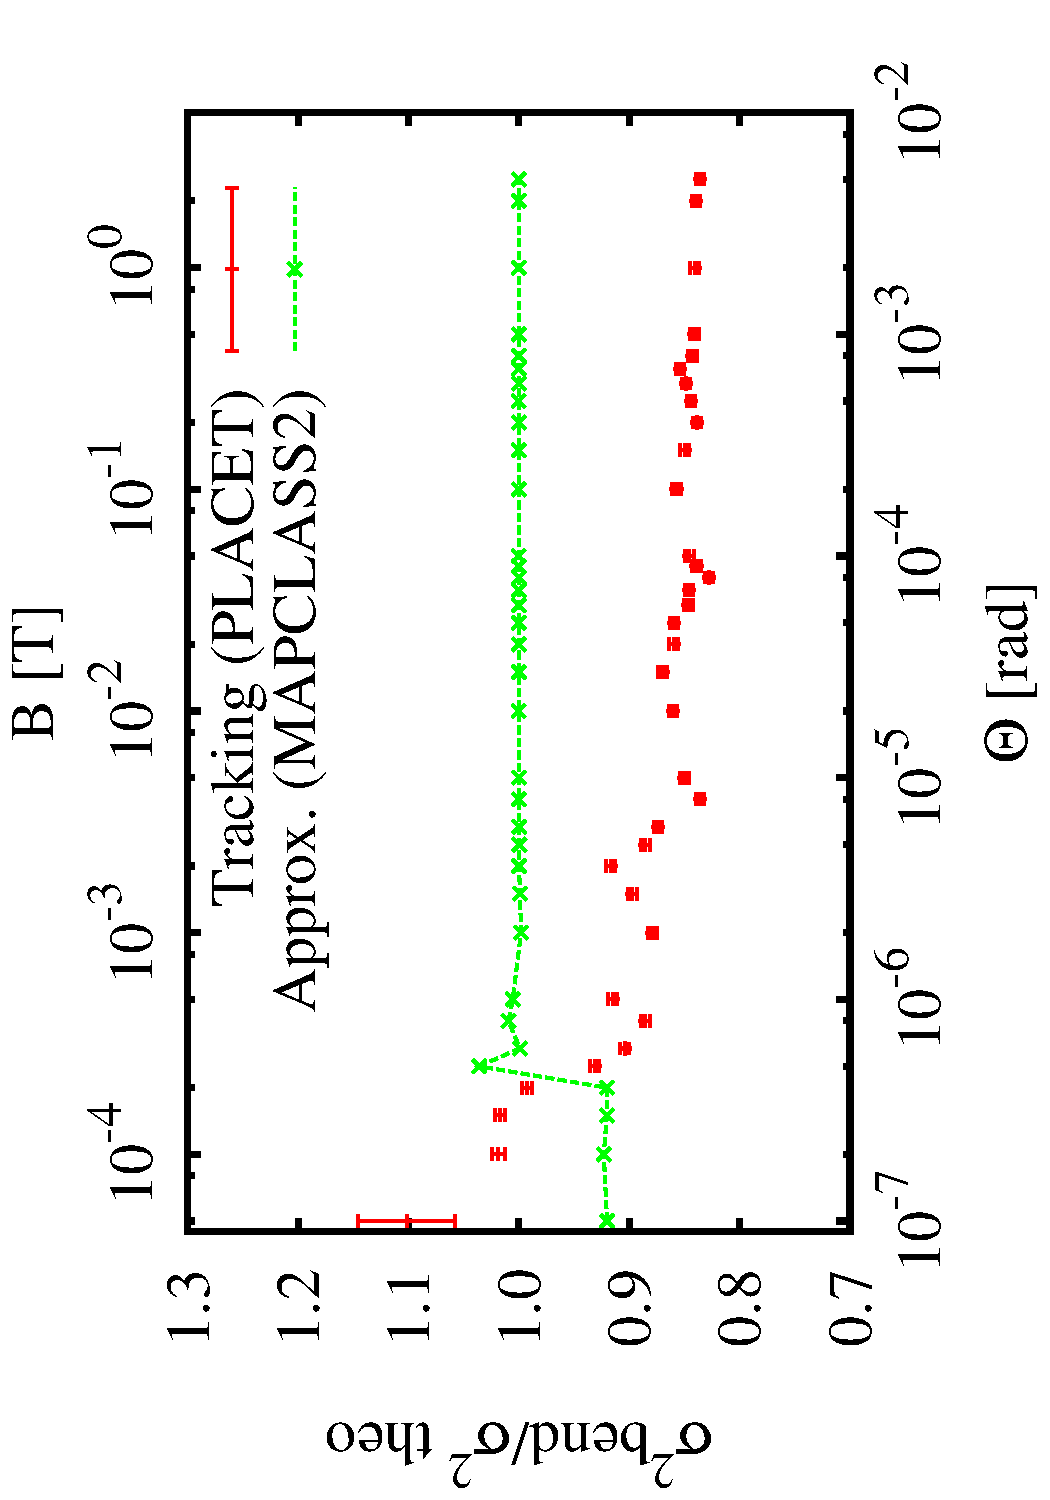
\includegraphics[scale=0.30,angle=-90]{sigma_angle.pdf}
  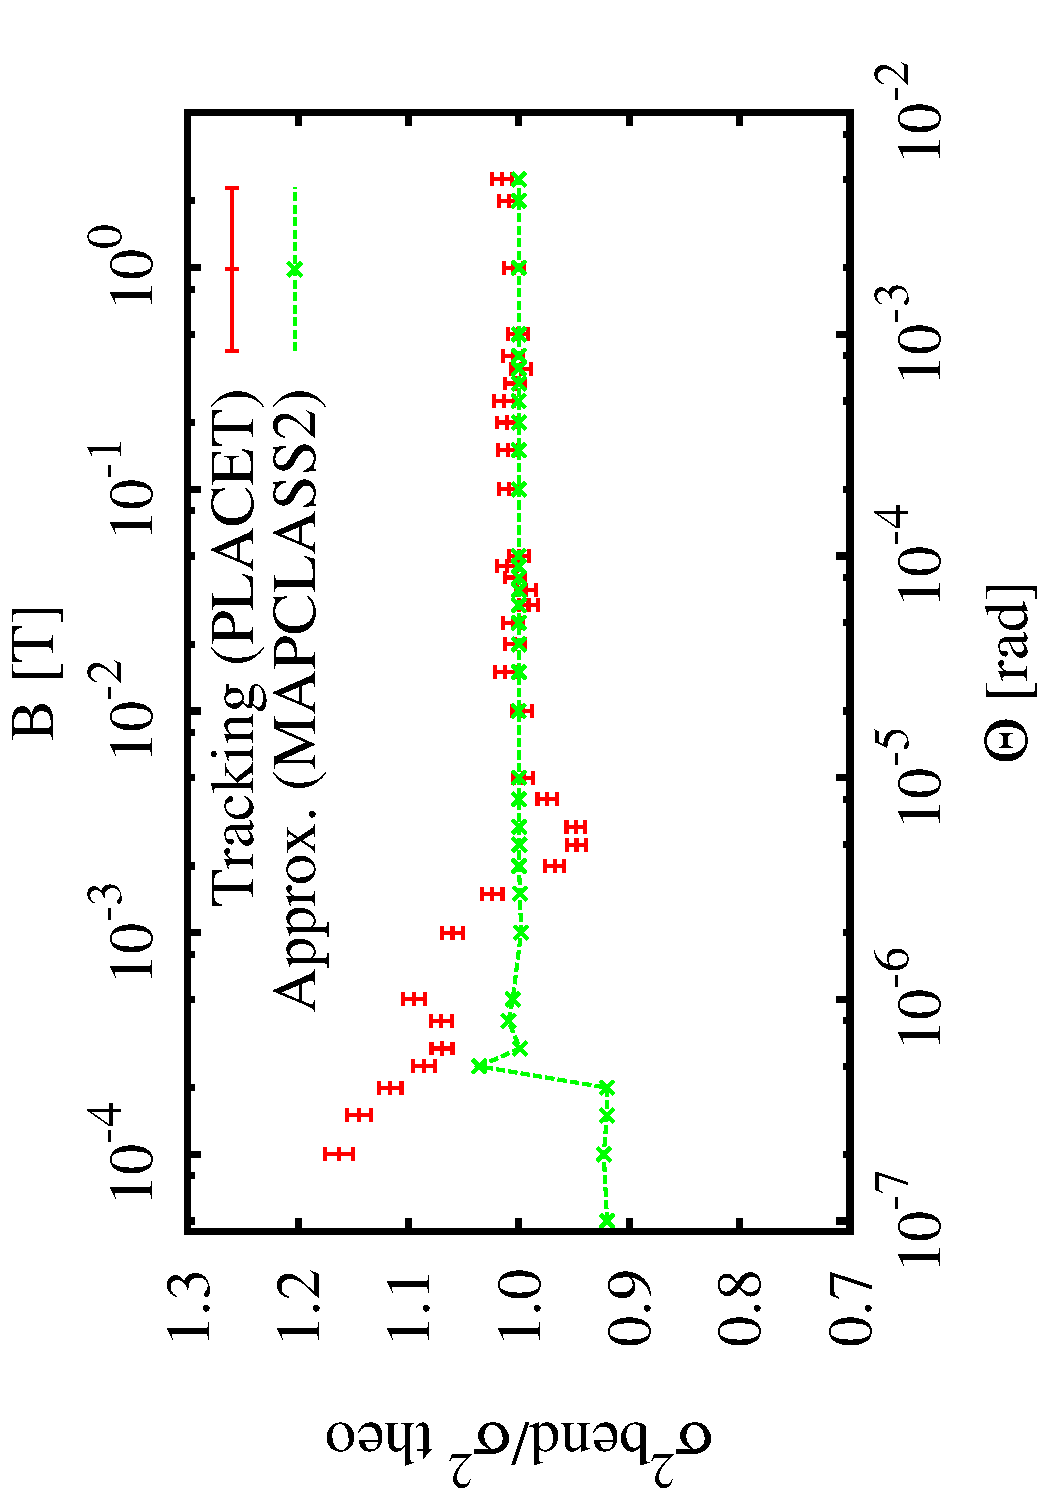
\includegraphics[scale=0.30,angle=-90]{sigma_angle_r06.pdf}\par
%   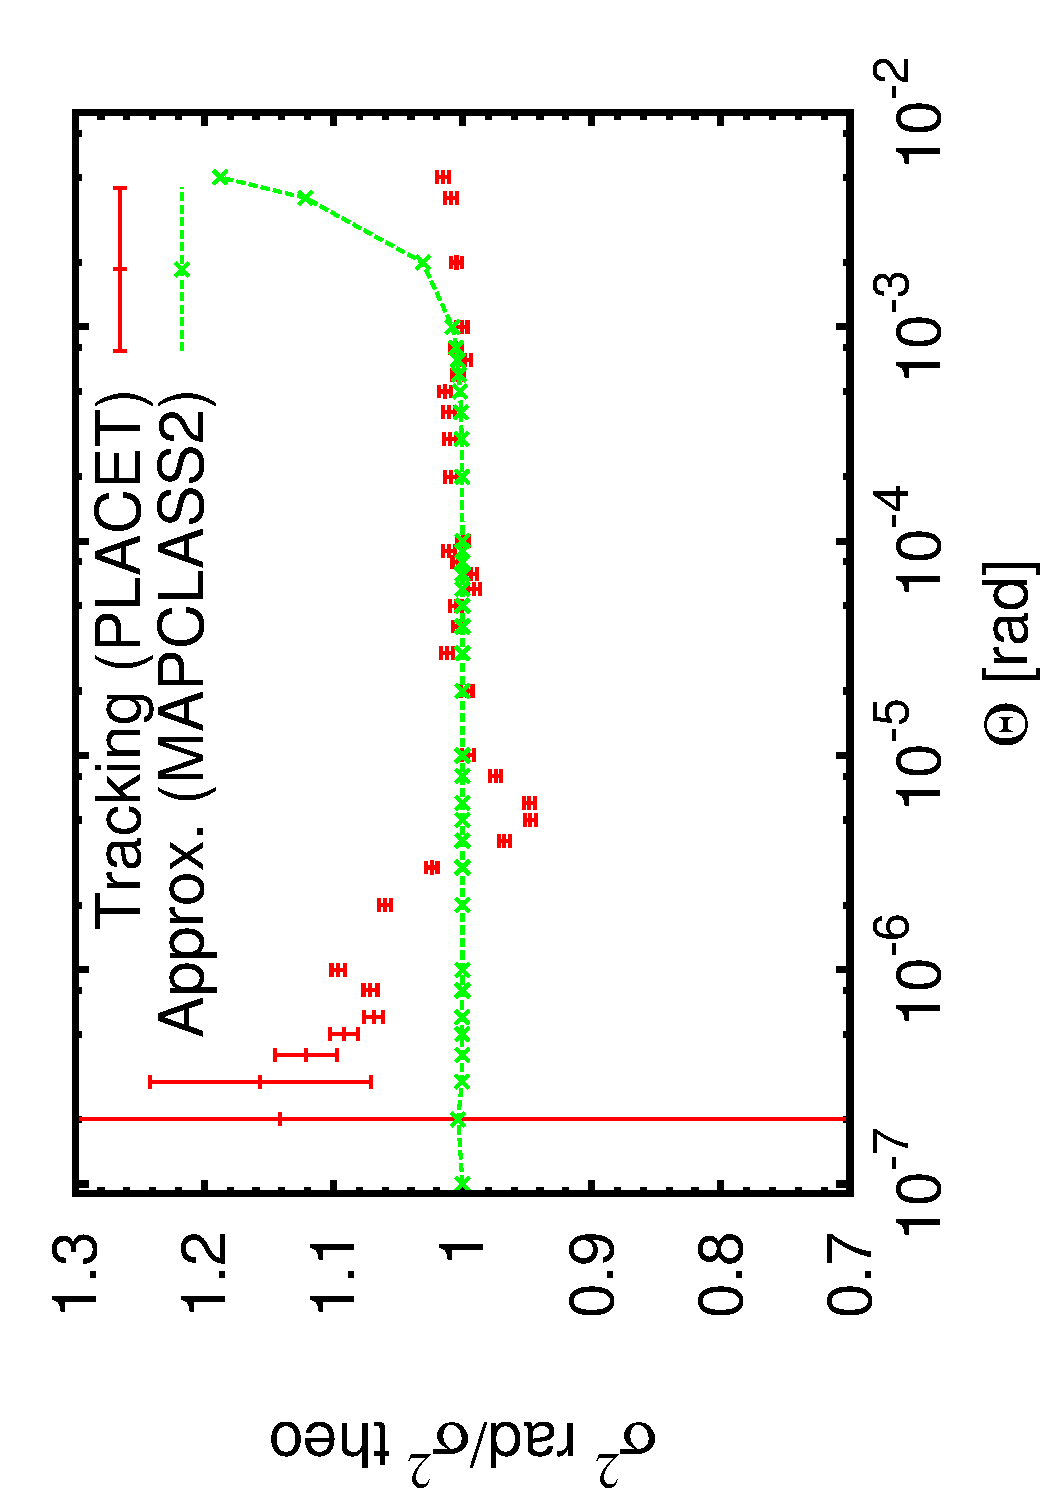
\includegraphics[scale=0.30,angle=-90]{sigma_angle_r6_twiss.pdf}\par
  \hspace*{1.0cm}(a)\hspace*{7.6cm}(b)\par
   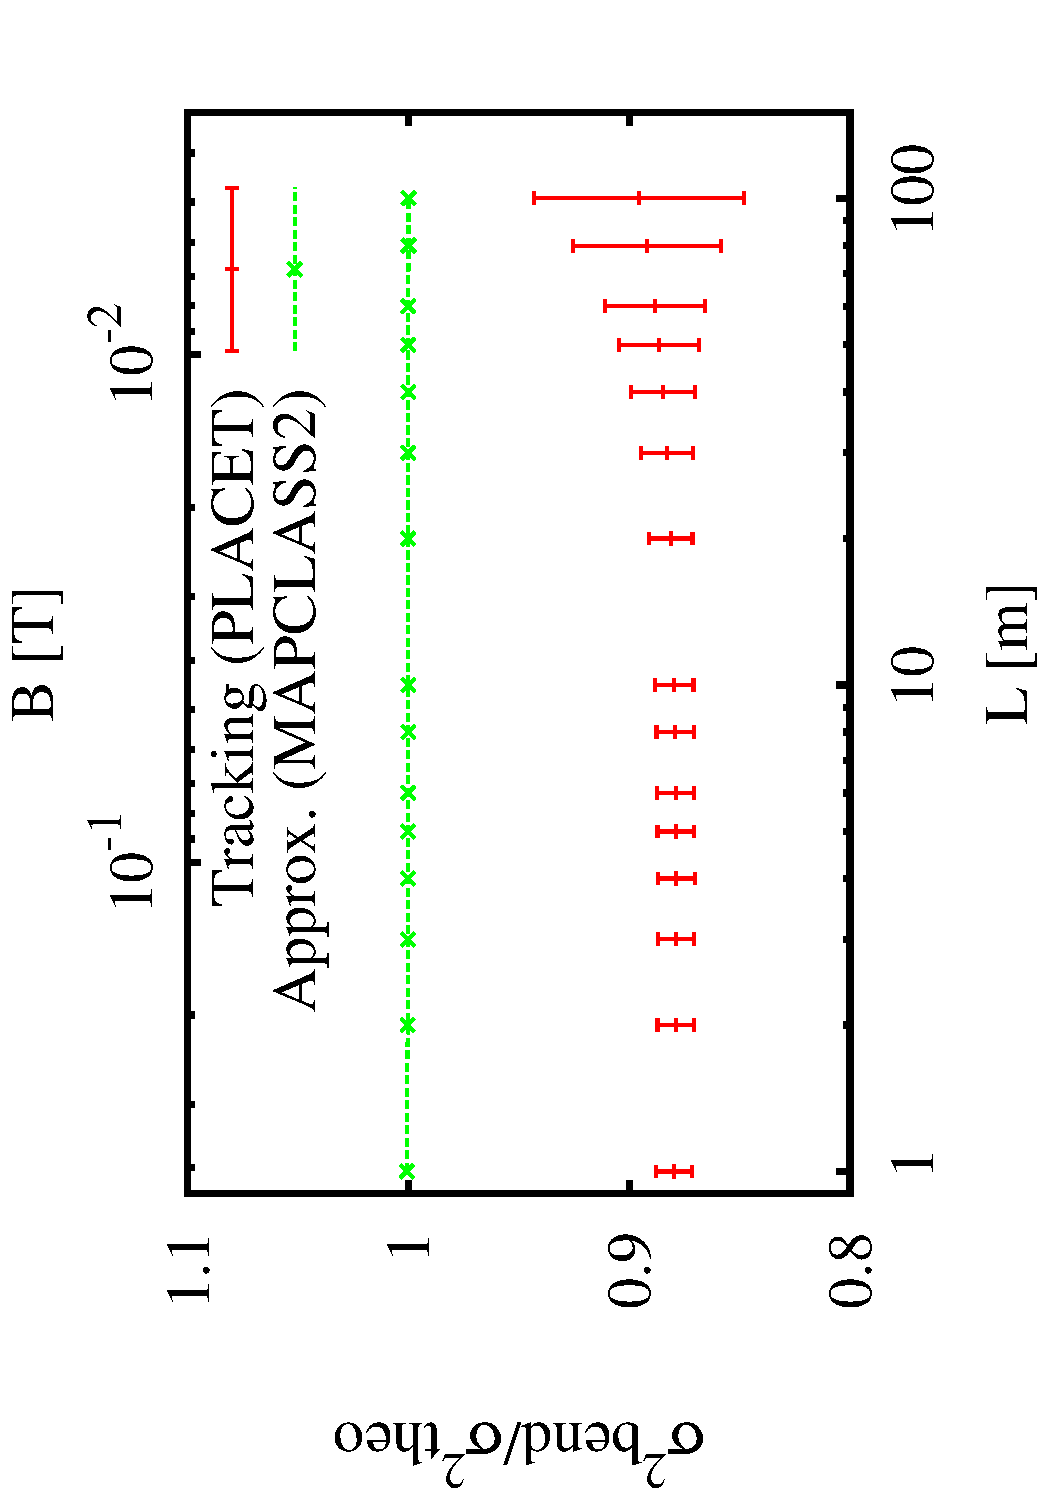
\includegraphics[scale=0.30,angle=-90]{sigma_Lbend.pdf}
  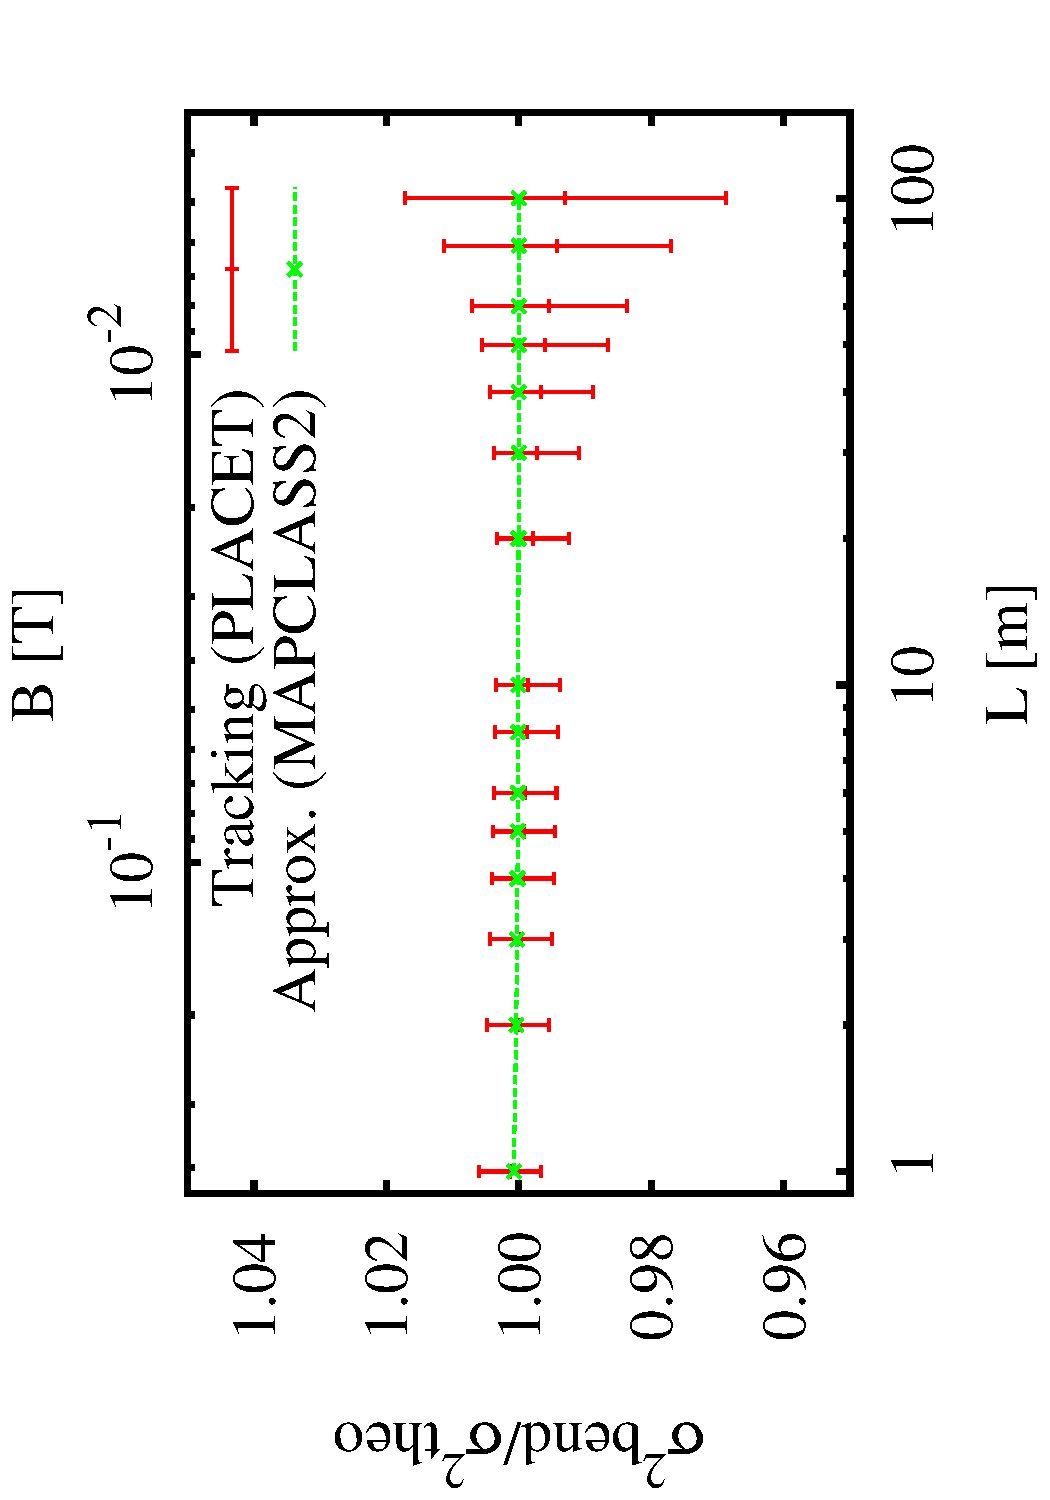
\includegraphics[scale=0.30,angle=-90]{sigma_Lbend_r6.pdf}\par
  \hspace*{1.0cm}(c)\hspace*{7.6cm}(d)\par
  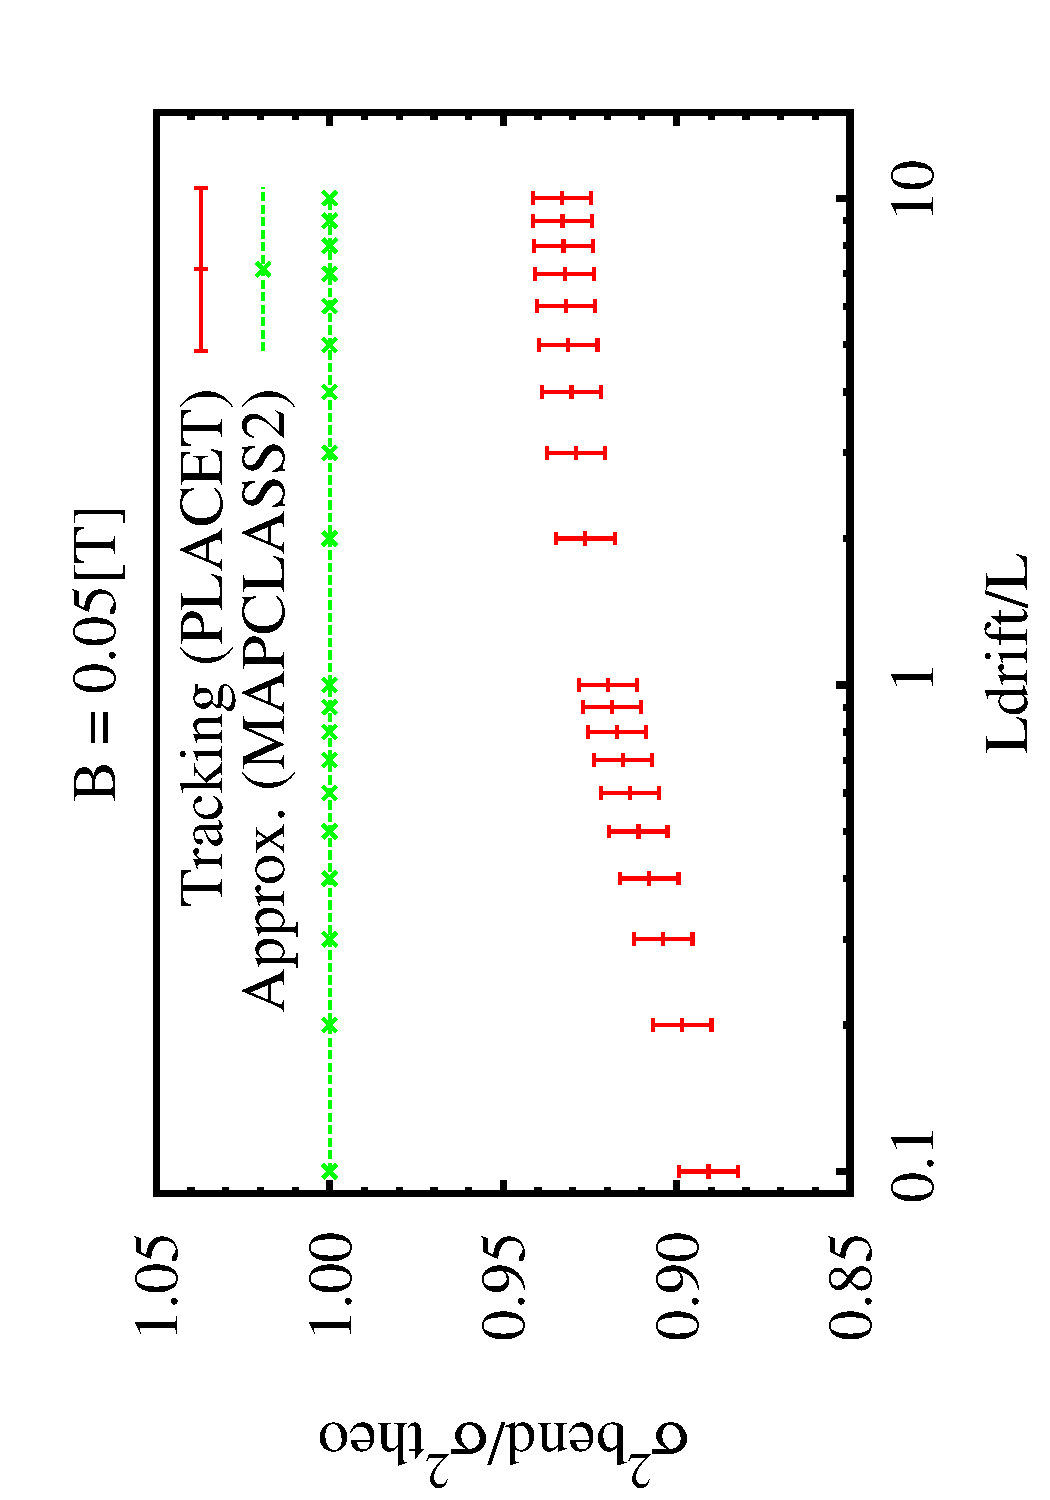
\includegraphics[scale=0.30,angle=-90]{sigma_Ldrift.pdf}
  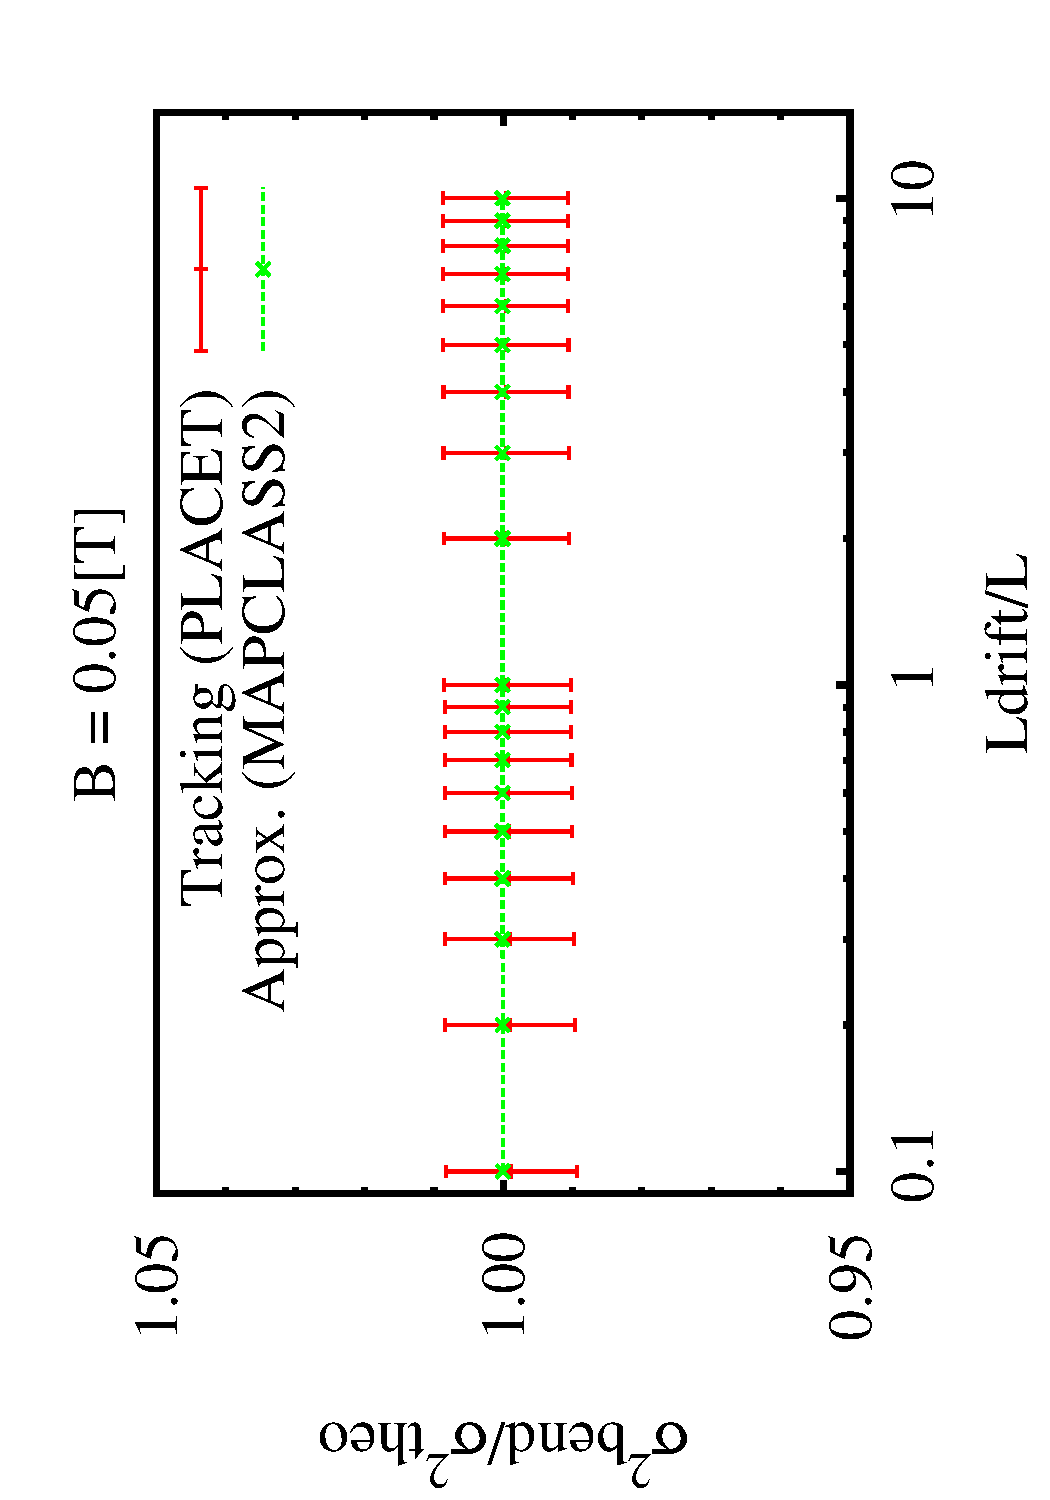
\includegraphics[scale=0.30,angle=-90]{sigma_Ldrift_r6.pdf}
  \hspace*{1.0cm}(e)\hspace*{7.6cm}(f)\par
\caption{Beam size increase due to radiation normalized to theoretical value assuming negligible energy loss. (Left) `Default' radiation option, (Right) `Six\_dim' option in PLACET 0.99.01. Plots (a) and (b) correspond to $L=10$ m for a dipole only. Plots (c) and (d) correspond to $\theta=10^{-4}$ rad for a dipole only. Plots (e) and (f) correspond to $L=10$ m and $\theta=10^{-4}$ rad while varying the drift length. Beam energy is 1500 GeV in all cases.}\label{figSR}
\end{figure}
\clearpage
\section{Model limitations}\label{s:modellim}
The radiation model reviewed is valid when the average number of photons radiated per particle $\langle N\rangle$ is enough to characterize the overall effect in position by its second moment, where $\langle N\rangle  = C_1E\theta$ with $C_1=20.61\text{ GeV}^{-1}$.\par
Although, Sect. \ref{s:comparison} explores the variation of $\theta$, it also changes the magnetic field strength $B$. Here, the magnetic field has been fixed $5 \times 10^{-3}$ T and the magnet length $L$ is systematically shorten to reduce the average number of photons emitted by each particle, equivalent to change $\theta$ because $B\rho$ is fixed for $E=1500$ GeV.\par
Fig. (\ref{figPhotons}) shows how the average number of photons emitted decreases with the dipole length $L$. It is visible also that the region where average is below one photon is also the starting point when tracking and theory start to differ, reaching $\pm10\%$ max.\par
This result is equivalent to the thin dipole approximation mentioned in Sect. \ref{s:comparison}, where the dipole sectioning makes of each slice a binomial trial of photon emission, approaching the Poisson theoretical distribution for large number of slices.\par
\begin{figure}[htb]
\centering
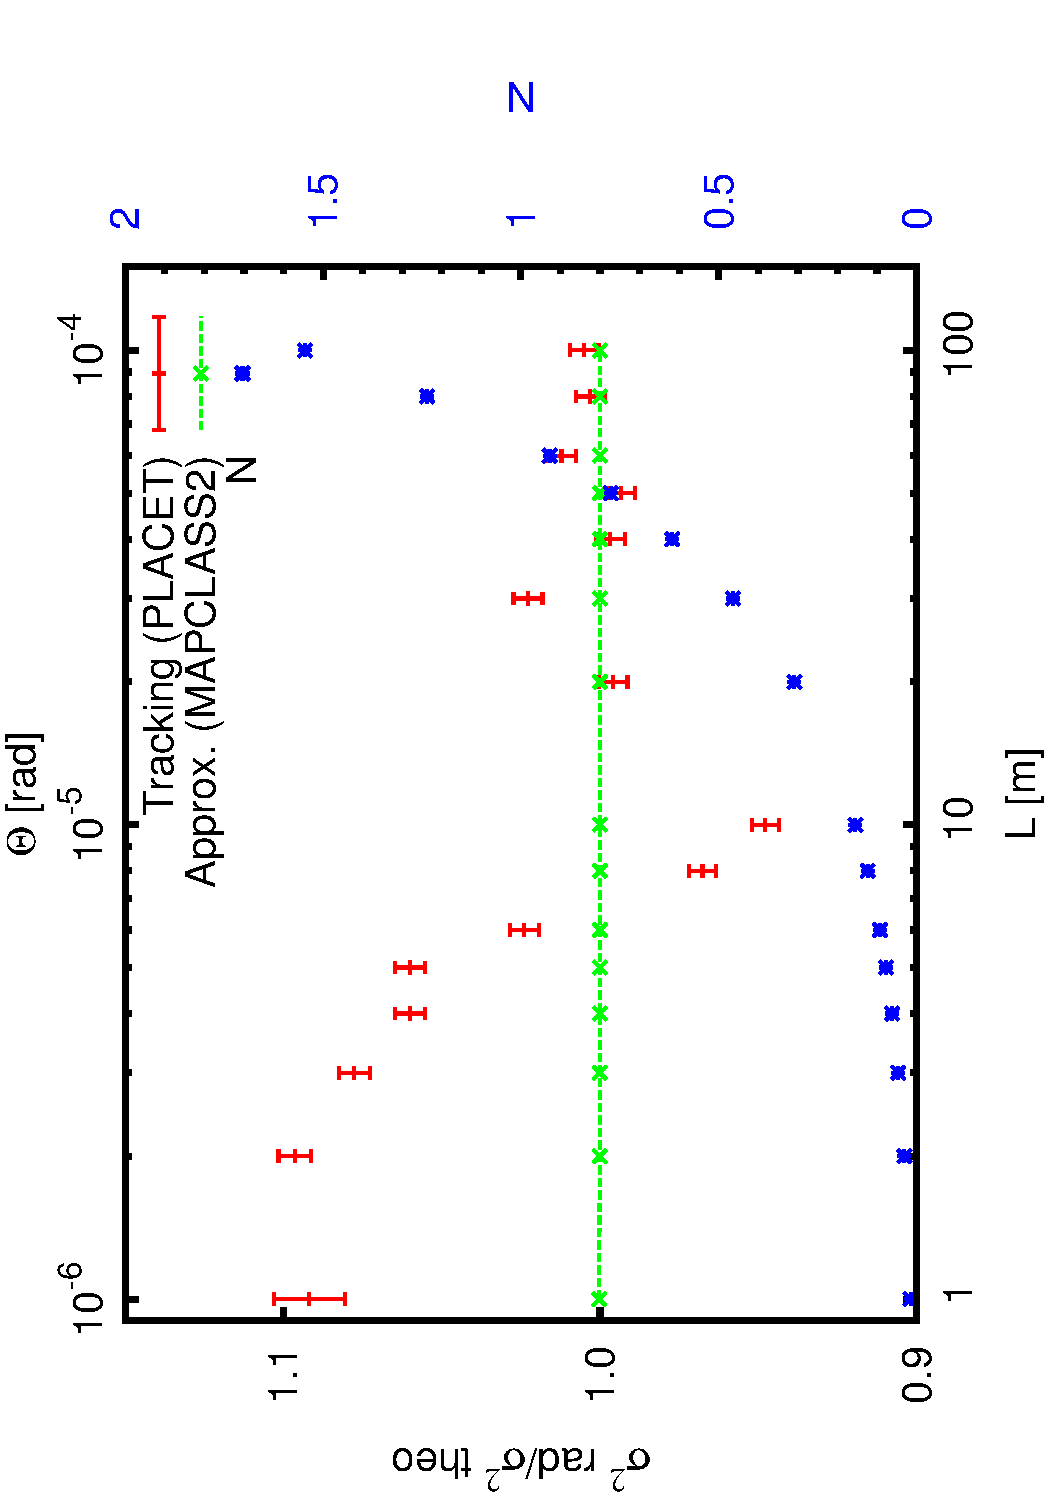
\includegraphics[scale=0.6,angle=-90]{./sigma_Bfix5e-3T.pdf} \caption{Result from tracking, theoretical calculation with the mean number of photons emitted by particle superimposed. Magnetic field is fixed at $5\times 10^{-3}$ T and $E=1500$  GeV.}\label{figPhotons}
\end{figure}

\section{Validity for the FFS}
The CLIC FFS design is composed by magnets with bending angles shown in Table \ref{T-nphotons_3TeV} for 3 TeV and Table \ref{T-nphotons_500GeV} for 500 GeV.  The third column indicates the quantity of magnets used in each of those sections.\par 
Although the average value of photons emitted per magnet is low, these are grouped in long sections with common bending angle. \begin{table}[ht]
\begin{minipage}[b]{0.45\linewidth}\centering
\begin{tabular}{c|c|c}\hline\hline
 $|\theta|$ & $\langle N \rangle$&Qty.\\
 ($\mu$rad)&&\\\hline
 $\;\;$1.1& 0.07 &70 \\
 $\;\;$3.9& 0.24 &20 \\
 17.2& 1.06 &10\\\hline
\end{tabular}\caption{Bending angles in CLIC 3 TeV.}\label{T-nphotons_3TeV}
\end{minipage}
\hspace{0.5cm}
\begin{minipage}[b]{0.45\linewidth}
\centering
\begin{tabular}{c|c|c}\hline\hline
 $|\theta|$& $\langle N \rangle$&Qty.\\
 ($\mu$rad)&&\\\hline
 $\;\;\;\;$8.3& 0.08&70\\
 $\;\;$27.5& 0.28 &20\\
 135.0& 1.39 &10\\\hline
\end{tabular}\caption{Bending angles in CLIC 500 GeV.}\label{T-nphotons_500GeV}
\end{minipage}
\end{table}
Using the conclusions from Sect. \ref{s:modellim} it will be similar to the thin dipole approximation and therefore the expression for beam size contribution from radiation in bending magnets should be within $\pm10\%$ agreement with tracking codes, making it useful for initial lattice optimization.\par

\chapter{Oide effect}
This part of the document addresses the radiation phenomenon in quadrupoles called Oide effect\cite{Oide}, which sets a limit on the beam size demagnification, specially important in linear colliders because of the strong focusing required in the Final Doublet before the Interation Point (IP).\par
First, a brief introduction to the beam size limit (Oide limit) is given, where calculations have been derived to include this radiation phenomenon in the lattice design and optimization software. The Oide effect is evaluated for the CLIC 3 TeV and CLIC 500 GeV parameters, leading to change the length of the first quadrupole before the IP, called QD0. It ends with a proposal to mitigate the impact of the Oide effect by adding correctors before and after the QD0, reducing the beam size.\par
\section{Beam size limit}\label{Oideeffect}
The Oide effect is caused by the interaction of charged particles with the magnetic field from quadrupoles. Radiation in a focusing magnet, schematically represented as QD0 in Fig. (\ref{f:Oideeffect}), changes the energy of the particle and modifies the focusing effect. This results in a limit on the minimum beam size specially relevant in the vertical plane.\par%For the horizontal direction, is mainly affected by radiation caused by the interaction of charged particles with the magnetic field from dipoles. %This report will be limited to sector dipoles or ``sbends''.\par
\begin{figure}[!hbt]
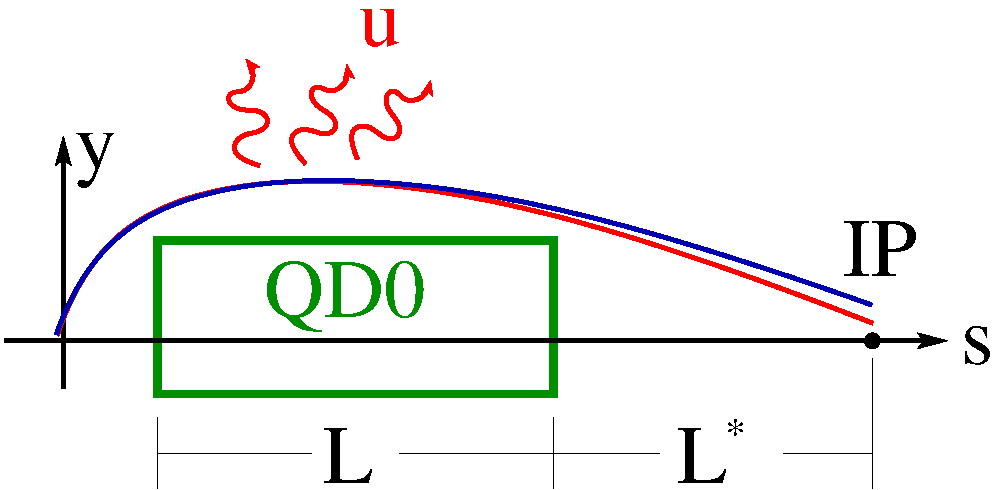
\includegraphics[scale=0.5]{Oide.pdf}
\centering
\caption{Design particle trajectory in blue and the trajectory of a particle due to radiation in the quadrupole in red.}\label{f:Oideeffect}
\end{figure}
 The beam size growth due to radiation is added quadratically to the linear beam size $\sigma_0^2=\epsilon\beta$ where $\beta$ represents the optical beta function and $\epsilon$ is the emittance. Therefore, $ \sigma^2 = \sigma_0^2 + \sigma_{oide}^2$, where the beam size contribution from the Oide effect is \cite{Oide},
 \begin{equation}
  \sigma^2_{oide} = \frac{110}{3\sqrt{6\pi}}r_e\frac{\lambda_e}{2\pi}\gamma^5 F(\sqrt{k}L,\sqrt{k}L^*)\left(\frac{\epsilon}{\beta^*}\right)^{5/2}
  \label{Oideequ}
 \end{equation}
 where
 \begin{equation}
  F(\sqrt{k}L, \sqrt{k}L^*) = \int_0^{\sqrt{k}L}|\sin\phi+\sqrt{k}L^*\cos\phi|^3\left[\int_0^\phi(\sin\phi'+\sqrt{k}L^*\cos\phi')^2 d\phi'\right]^2d\phi
  \label{OideF}
 \end{equation}
  and $\lambda_e$ is the Compton wavelength of the electron, $r_e$ is the classical electron radius, $\gamma$ is the relativistic factor, $\epsilon$ is the geometrical beam emittance, $\beta^*$ is the Twiss parameter at the observation point (in this case, the IP), and $k$, $L$ and $L^*$ are the quadrupole gradient, the quadrupole length and the distance to the observation point measured from the closest magnet face.\par
   Although the total contribution to beam size depends on the lattice and beam parameters, the minimum achievable beam size is given by \cite{Oide}
%the function $F$ is calculated only from quadrupole parameters. For this reason, $F$ will be used as figure of merit for a quadrupole.
\begin{equation}
 \sigma_{y \text{ min}} = \left(\frac{7}{5}\right)^\frac{1}{2}\left[\frac{275}{3\sqrt{6\pi}}r_e\frac{\lambda_e}{2\pi}F(\sqrt{K}L,\sqrt{K}L^*)\right]^\frac{1}{7}(\epsilon_{Ny})^\frac{5}{7}
\end{equation}
where $\epsilon_N=\gamma\epsilon$ is the normalized emittance, showing the independence from beam energy.\par
The only possibility to reduce the beam size is by changing the value of $F$, by modifying the magnet parameters, or to minimize the beam emittance. However, using the ILC 500 GeV \cite{ILCdes}, CLIC 500 GeV and CLIC 3 TeV \cite{CLICdes} parameters, it is possible to conclude from columns $\sigma_0$ and $\sigma_{oide}$ in Table (\ref{t:Sigmas}) that the contribution of the Oide effect to beam size is only significant for CLIC 3 TeV.\par
In addition, columns $\sigma$ and $\sigma_{min}$ in Table (\ref{t:Sigmas}) show that both CLIC designs are close to the minimum achievable beam size.\par
\begin{table}[!hbt]
\centering
{\scriptsize
\begin{tabular}{l||c|c|c||c|c|c|c|c||c|c}\hline\hline
Lattice &$\epsilon_N$& $\gamma$& $\sigma_0$&$k$&$L$&$L^*$& $F$ & $\sigma_{oide}$&$\sigma$&$\sigma_{min}$\\
 &(nm)&($10^3$)&(nm)&(m$^{-2}$)&(m)&(m)&&(nm) &(nm)&(nm)\\\hline
CLIC 3 TeV & 20 & 2935.0 & 0.70 & 0.116 & 2.73 &3.5&  4.086  & 0.85 & 1.10& 1.00 \\
CLIC 500 GeV & 25 & $\;\;$489.2 & 2.3 & 0.077 & 3.35 &4.3& 4.115 & 0.08 & 2.3 & 1.17\\
ILC  500 GeV & 40 & $\;\;$489.2 & 5.7 & 0.170 & 2.20 &4.3& 9.567 & 0.04 & 5.7 & 1.85\\\hline
\end{tabular}\caption{Vertical beam size and radiation beam size contribution for three lattices. $\epsilon_N$ is the normalized emittance, $\epsilon_N=\gamma\epsilon$.}\label{t:Sigmas}
}
\end{table}

\section{Oide Double Integral Solution}\label{s:DoubleIntegral}
In this section the double integral used to calculate $F$ is solved with the goal to increase the computational calculation speed. It was included in MapClass2\cite{Mapclassorig,Mapclass,Mapclass2,githubMapClass2} to be used in lattice design and optimization.\par
  The inner integral over $\phi'$ can be solved because it has a known primitive.
\begin{equation}
 \int_0^\phi (\sin \phi'+ \sqrt{k}l^*\cos\phi')^2d\phi'=\frac{\phi}{2}[(\sqrt{k}l^*)^2 +1 ] + \frac{\sin(2\phi)}{4}[(\sqrt{k}l^*)^2 -1]+\sqrt{k}l^*\sin^2\phi
\end{equation}
The Eq. (\ref{OideF}) can now be expressed as one integral.
{\scriptsize
\begin{align}
F(\sqrt{k}L&,\sqrt{k}l^*) =\\
&\int_0^{ \sqrt{k}L} |\sin\phi+\sqrt{k}l^*\cos\phi|^3 \left( \frac{\phi}{2}[(\sqrt{k}l^*)^2 +1 ] + \frac{\sin(2\phi)}{4}[(\sqrt{k}l^*)^2 -1]+\sqrt{k}l^*\sin^2\phi\right)^2 d\phi\notag
\end{align}
}
The squared factor in brackets is always positive because all inner terms are real. The term inside the absolute value is also always positive, therefore, the integrand is always positive. Now, considering the function:
  \begin{equation}
  |\sin \phi + \sqrt{k}l^*\cos\phi|=\left\{
  \begin{array}{c l l}
&  \sin\phi+\sqrt{k}l^*\cos	\phi,\quad\qquad&\text{if}, \sin\phi+	\sqrt{k}l^*\cos	\phi\geq0\\
&  -(\sin\phi+\sqrt{k}l^*\cos\phi),\quad&\text{if}, \sin\phi+	\sqrt{k}l^*\cos	\phi<0
  \end{array}\right.\label{eq-absval}
 \end{equation}
sign changes at every point $\quad\phi_n = \arctan(-\sqrt{ k}l^*)\pm n\pi,\quad n\geq1$.\par
It is possible to split the integration interval $i$ times, being $i$ the number of $\phi_n$ solutions where $0<\phi_n<\sqrt{k}L$. On each of those intervals, the absolute value definition can be removed and replaced by the corresponding expression in Eq. (\ref{eq-absval}), having only a difference in sign. By defining the primitive $\mathscr{F}$ in an interval where the factor inside the absolute value is positive it is possible to evaluate $F$ as it is shown in Eq. (\ref{eq-primeval}).
\begin{equation}
 F(\sqrt{k}L,\sqrt{k}l^*)= \mathscr{F}|_0^{\phi_1} - \mathscr{F}|_{\phi_1}^{\phi_2} +  \mathscr{F}|_{\phi_2}^{\phi_3} - \mathscr{F}|_{\phi_3}^{\phi_4}+ \cdots \pm  \mathscr{F}|_{\phi_i}^{\sqrt{k}L}\label{eq-primeval}
\end{equation}
The change of signs in each interval is only  given by the absolute value definition, then, it is simpler to add the absolute value of each contribution.
\begin{equation}
 F(\sqrt{k}L,\sqrt{k}l^*)= \bigr\vert\mathscr{F}|_0^{\phi_1}\bigr\vert + \bigr\vert\mathscr{F}|_{\phi_1}^{\phi_2}\bigr\vert +  \bigr\vert\mathscr{F}|_{\phi_2}^{\phi_3}\bigr\vert + \bigr\vert\mathscr{F}|_{\phi_3}^{\phi_4}\bigr\vert + \cdots +\bigr\vert\mathscr{F}|_{\phi_i}^{\sqrt{k}L}\bigr\vert
\end{equation}
If we know the primitive $\mathscr{F}$ and we are able to calculate the $\phi_n$s in the integration interval, then, it is possible to calculate the factor $F$ without using an approximate integrator. The double integration has been simplified to a primitive evaluation.\par
The primitive $\mathscr{F}$ exists and it has been calculated using Maxima \cite{Maxima} and Wolfram Alpha Mathematica\cite{Wolfram} software, the expression is in Appendix \ref{c:primitiveF}.\par
  
 
\section{Mitigating the impact on the beam size}
\subsection{QD0 length}
As shown in Sect. \ref{Oideeffect} the Oide beam size contribution depends on a combination of beam and optics parameters. %Table \ref{tabSigmas} gives the results.
If none of the beam parameters is to be changed then $F$ can be used as a figure of merit of the optics as it is calculated only from $k$, $L$ and $l^*$. The target is to reduce it as much as possible. Two energy cases are analyzed in the following: 3 TeV ($l^*=3.5$ m) and 500 GeV ($l^*=4.3$ m).\par
Columns $\sigma_0$, $\sigma_{oide}$ and $F$ in Table \ref{t:Sigmas} show that CLIC 3 TeV and 500 GeV \cite{CLICdes,TomasCLIC} have larger contributions to beam size even having a lower $F$ value than ILC 500 GeV \cite{ILCdes}.\par
In order to evaluate the minimum possible $F$ for $l^*$ given, the minimum $k$ required to get the particles focused is when the Twiss function $\alpha$ is zero just at the quadrupole opposite face to the IP.\par
Figure \ref{fig-3TeV:a}  shows the ratio squared between the beam size contribution due to Oide effect and the linear beam size for three cases: when $k$ is the minimum required to get particles focused (to get $\alpha_y=0$ at QD0 opposite side to the IP), when $k$ is calculated as thin lens ($k=\frac{1}{Ll^*}$), and the current QD0 status. Fig. \ref{fig-3TeV:b} shows the $k$ values for the previous mentioned cases.\par
The Oide contribution to beam size is of the same order of the linear beam size. It might be possible to reduce it by doubling the current quad length and using a lower $k$ between the minimum required for the focusing and the thin lens approximation. This also points to increasing the lattice length as this change reduces the tolerance to variations of $\alpha$ at the quadrupole input.\par
Quad lengths larger than 10 m do not lead to further improvements with the current parameters.\par

\begin{figure}[!htb]
\centering
\hspace*{-0.6cm}
\begin{subfigure}{0.45\textwidth}
\centering
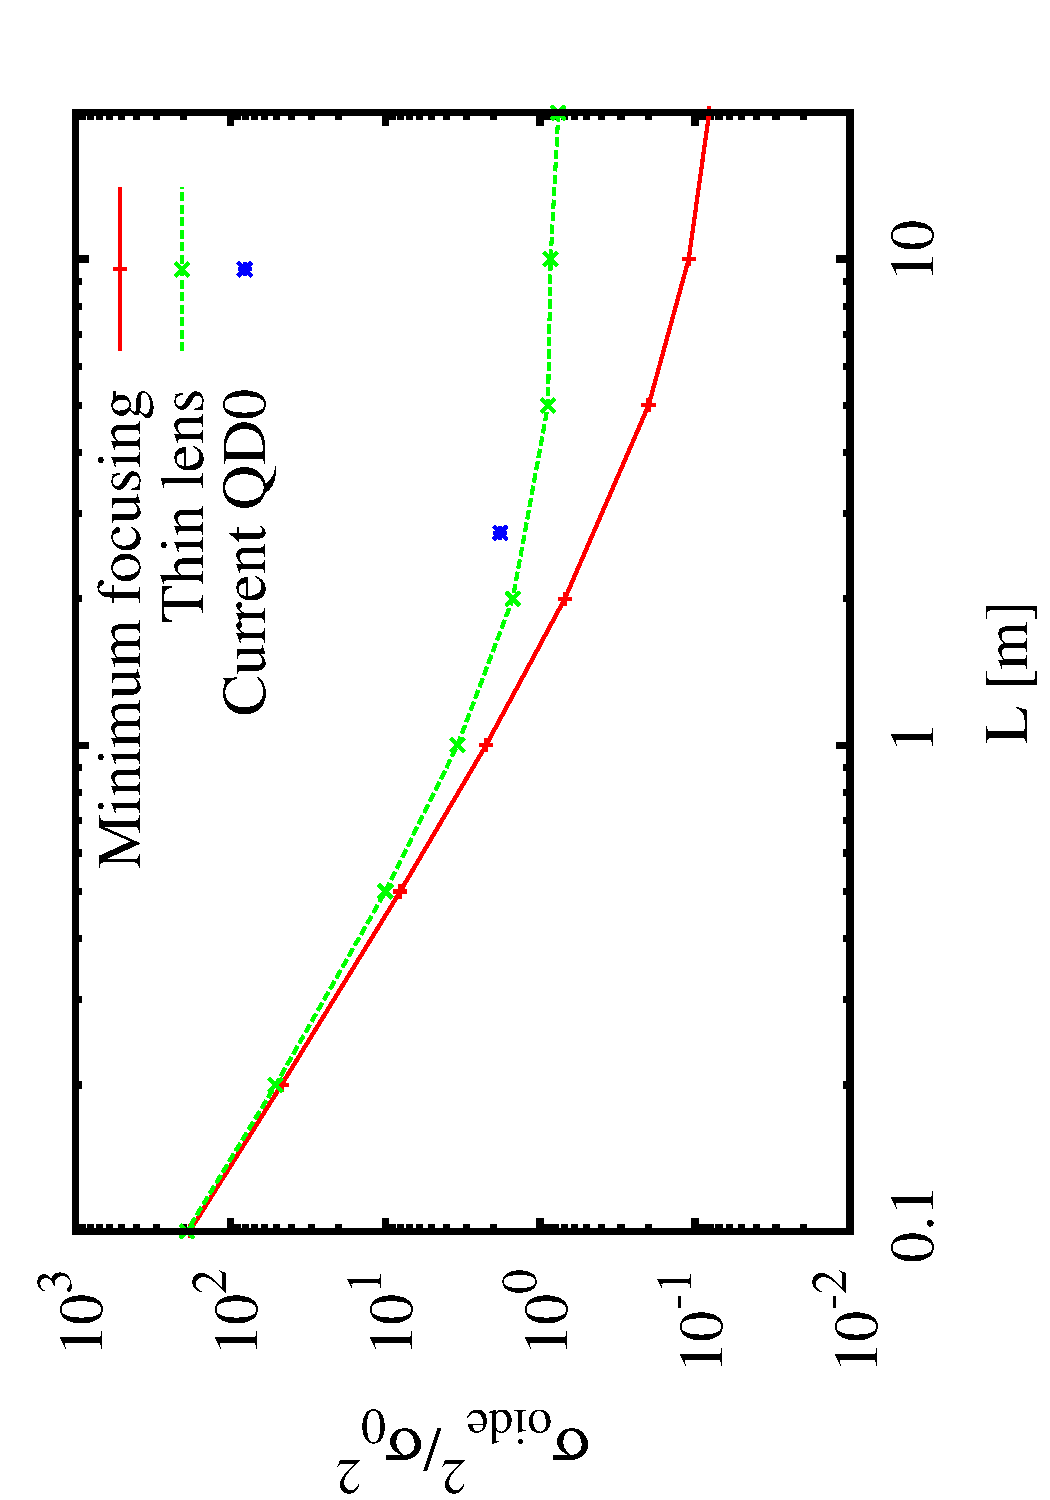
\includegraphics[scale=0.3,angle=-90]{image07a.pdf}\caption{}\label{fig-3TeV:a}
\end{subfigure}
\begin{subfigure}{0.45\textwidth}
\centering
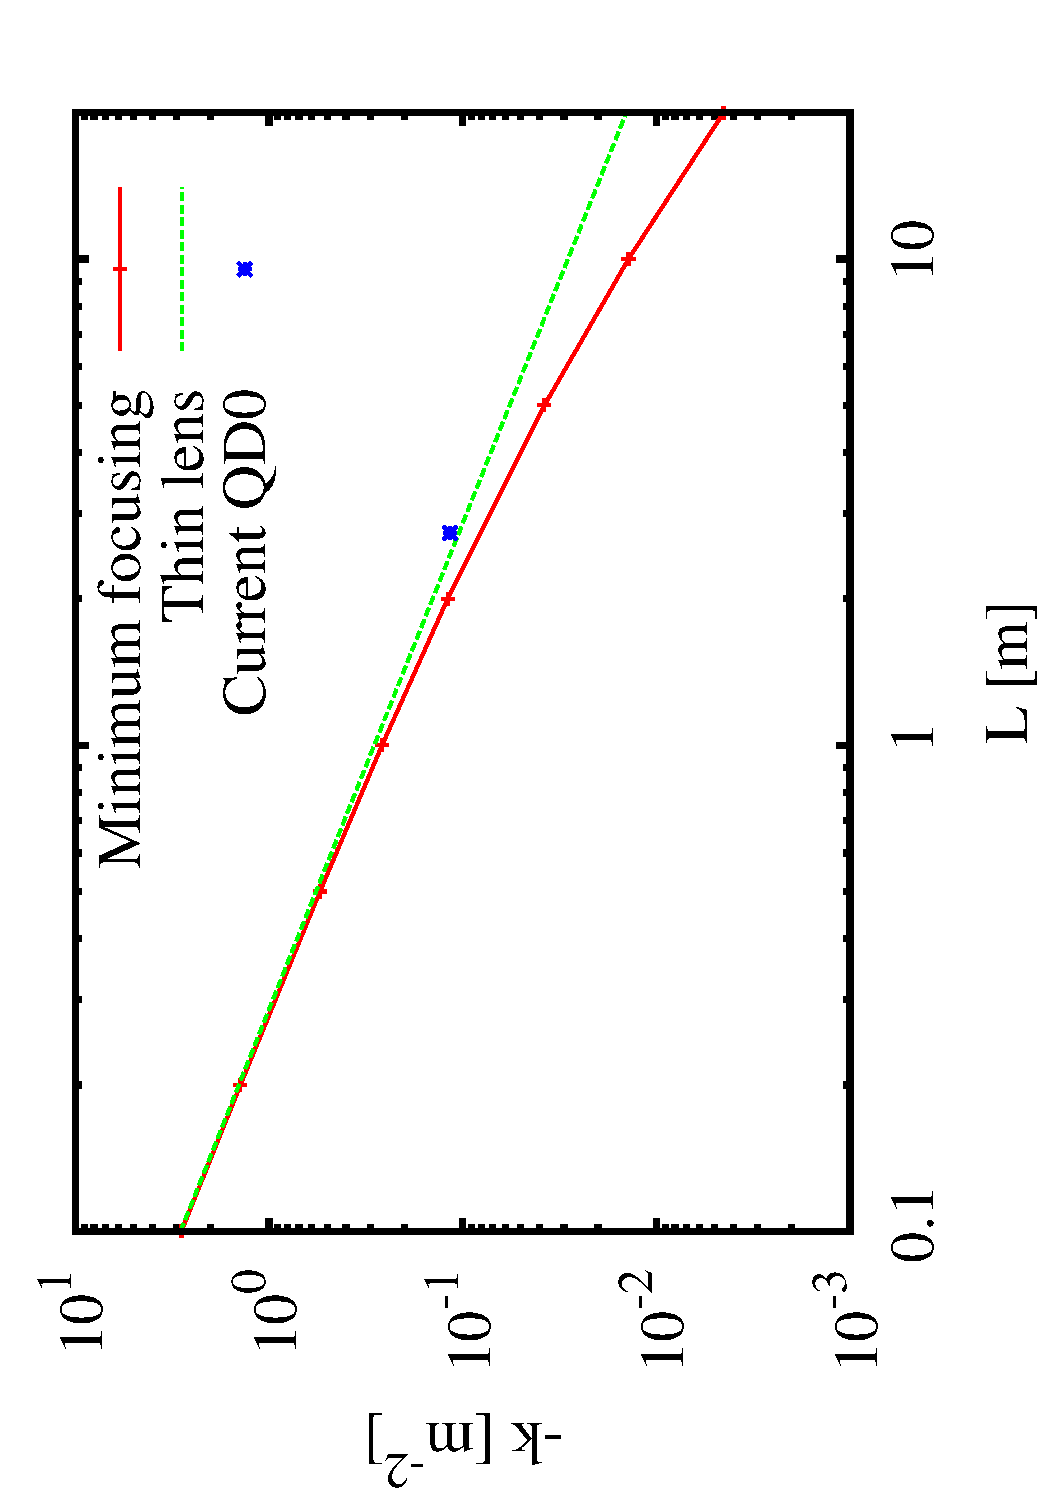
\includegraphics[scale=0.3,angle=-90]{image07b.pdf}\caption{}\label{fig-3TeV:b}
\end{subfigure}
\caption{Oide effect beam size contribution for CLIC 3 TeV design parameters. (a) $\sigma^2_{oide}$ normalized to designed linear beam size as a function of quad length for the minimum focusing $k$ (when $\alpha_y=0$ at the quadrupole opposite side to the IP), for $k$ calculated as thin lens ($k=\frac{1}{Ll^*}$) and the current QD0. (b) $k$ in the three previous cases for comparison.}\label{fig-3TeV}	
 \end{figure}\par
Figure \ref{fig-500GeV} is the corresponding to Fig. \ref{fig-3TeV} for the 500 GeV case. The current design contributes less than 4\% of the total beam size, concluding that the current QD0 length with the CLIC 500 GeV parameters does not need adjustment.\par
\begin{figure}[!htb]
\centering
\hspace*{-0.6cm}
\begin{subfigure}{0.45\textwidth}
\centering
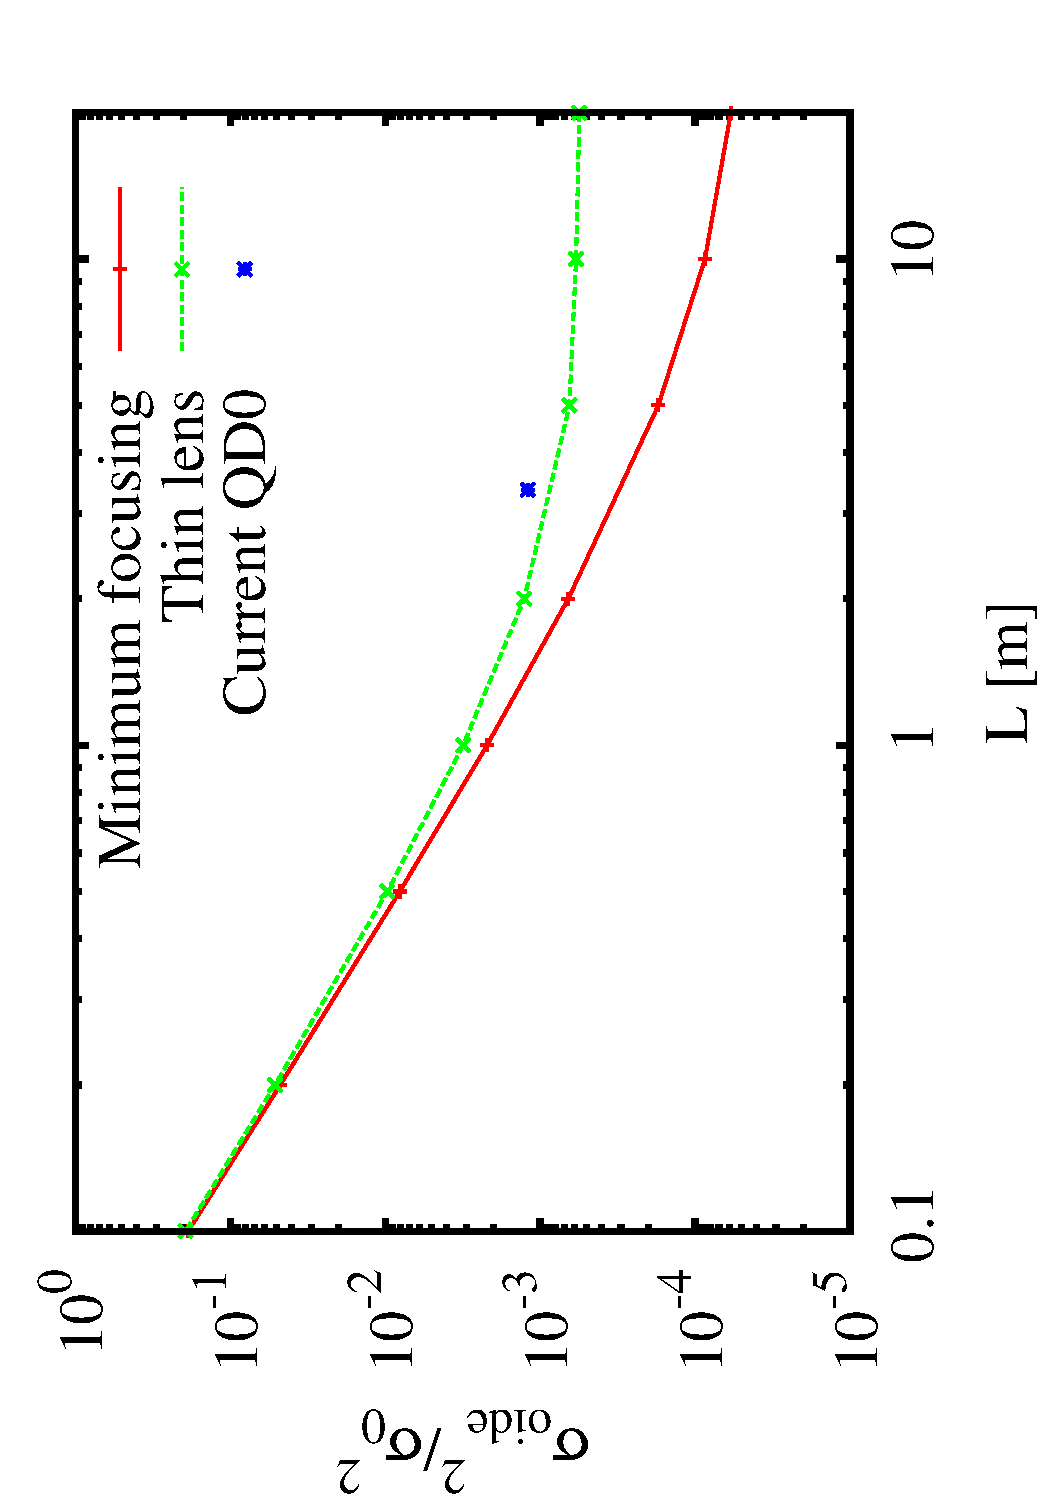
\includegraphics[scale=0.3,angle=-90]{image06b.pdf}\caption{}
\end{subfigure}
\begin{subfigure}{0.45\textwidth}
\centering
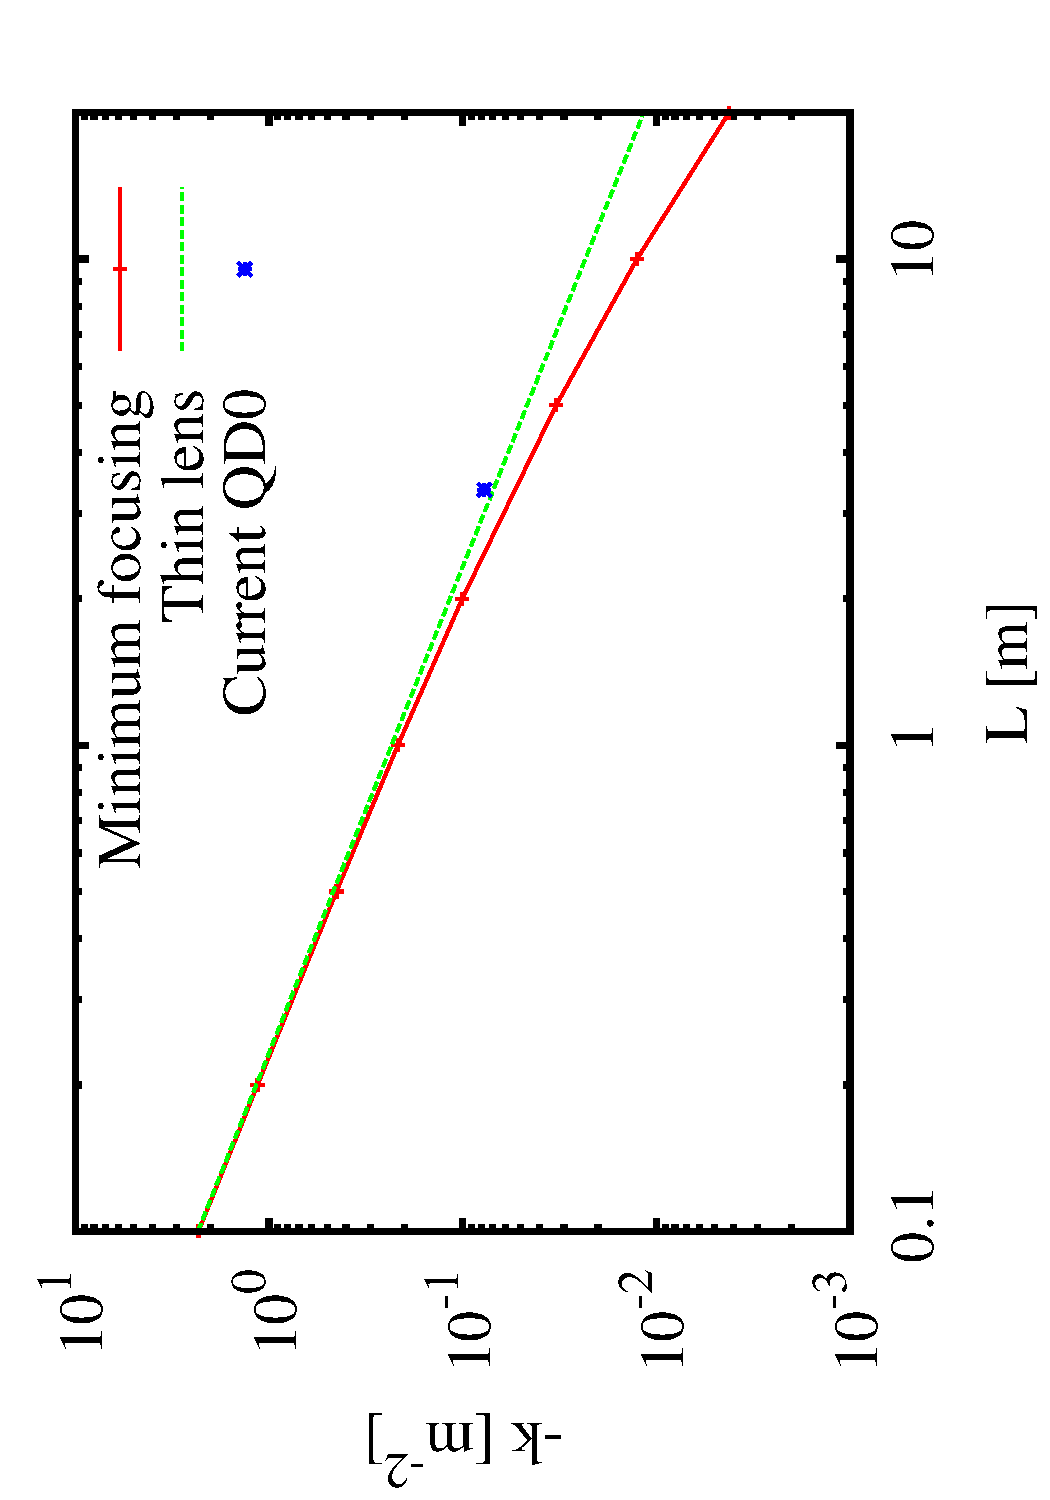
\includegraphics[scale=0.3,angle=-90]{image06c.pdf}\caption{}
\end{subfigure}
\caption{Oide effect beam size contribution for CLIC 500 GeV design parameters. (a) $\sigma^2_{oide}$ normalized to designed linear beam size as a function of quad length for the minimum focusing $k$ (when $\alpha_y=0$ at the quadrupole opposite side to the IP), for $k$ calculated as thin lens ($k=\frac{1}{Ll^*}$) and the current QD0. (b) $k$ in the three previous cases for comparison.}\label{fig-500GeV}
 \end{figure}\par	

\subsection{Correctors}
\subsubsection{$\Delta y$ due to radiation}
Particle tracking from the imput of QD0 to the IP for CLIC 3 TeV with and without radiation, using PLACET \cite{Placet}, allows one to compute the effects of radiation on the six dimentional phase space. Figure \ref{f:CLIC3TeVbeamsizeIP} shows the current transverse distribution of particles at the IP. To compensate the adverse effects a compensation system would ideally remove the position change due to radiation $\Delta y = y_\text{rad} -y_0$.\par
\begin{figure}[!htb]
\centering
 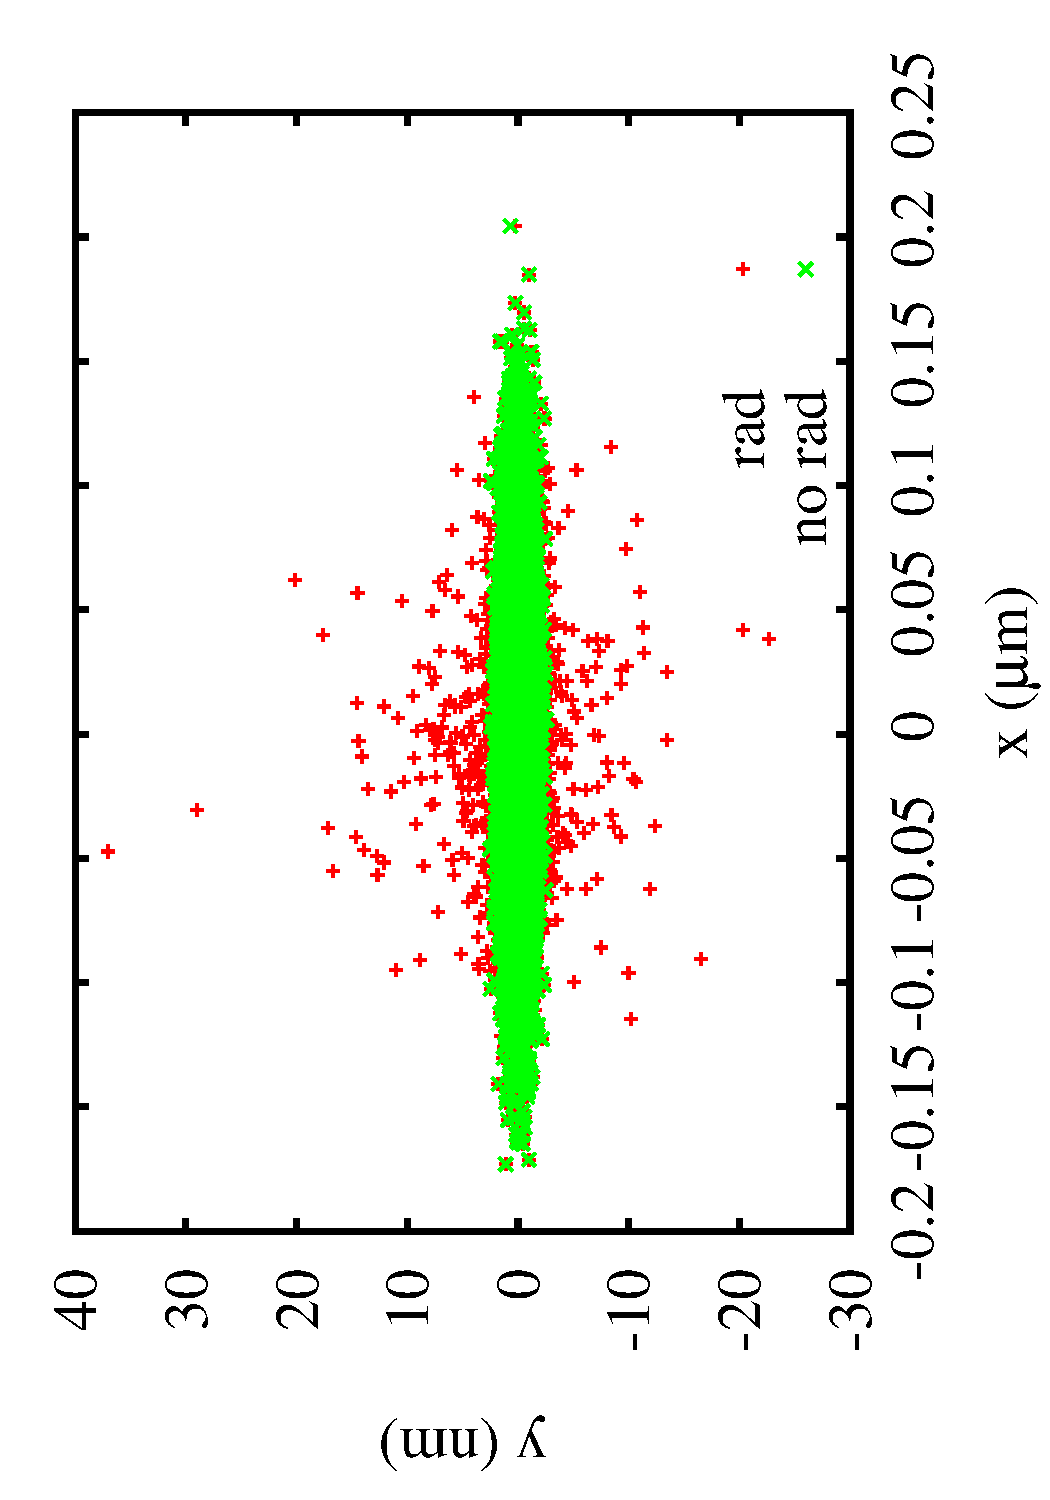
\includegraphics[scale=0.3,angle=-90]{plotxyrad.pdf}\caption{CLIC 3 TeV beam at the IP after tracking through 	QD0 with and without radiation.}\label{f:CLIC3TeVbeamsizeIP}
\end{figure}
Although the average radiation effect is zero, $\langle \Delta y \rangle = 0$ because of the cubic term $(y_0')^3$ as stated by Oide \cite{Oide}, the correlation between $\Delta y, y'$ is not zero. The correlation expression is shown in Eq. (\ref{eq:deltamean}).
\begin{equation}
 \langle\Delta y,y'_0\rangle = \frac{2}{3}r_e\gamma^3G(\sqrt{K}L,\sqrt{K}L^*)(y'_0)^3\label{eq:deltamean}
\end{equation}
%$r_e$ is the clasical electron radius and 
where $G(\sqrt{K}L,\sqrt{K}L^*)$ is given by
\begin{equation}
\int_0^{\sqrt{K}L}(\sin\phi+\sqrt{K}L^*\cos\phi)^2\int_0^\phi (\sin\phi'+\sqrt{K}L^*\cos\phi')^2 d\phi'd\phi
\end{equation}
Fig. \ref{f:correlation} shows the comparison between the correlation obtained from tracking and the theoretical evaluation of the previous expression.\par
\begin{figure}[!htb]
\centering
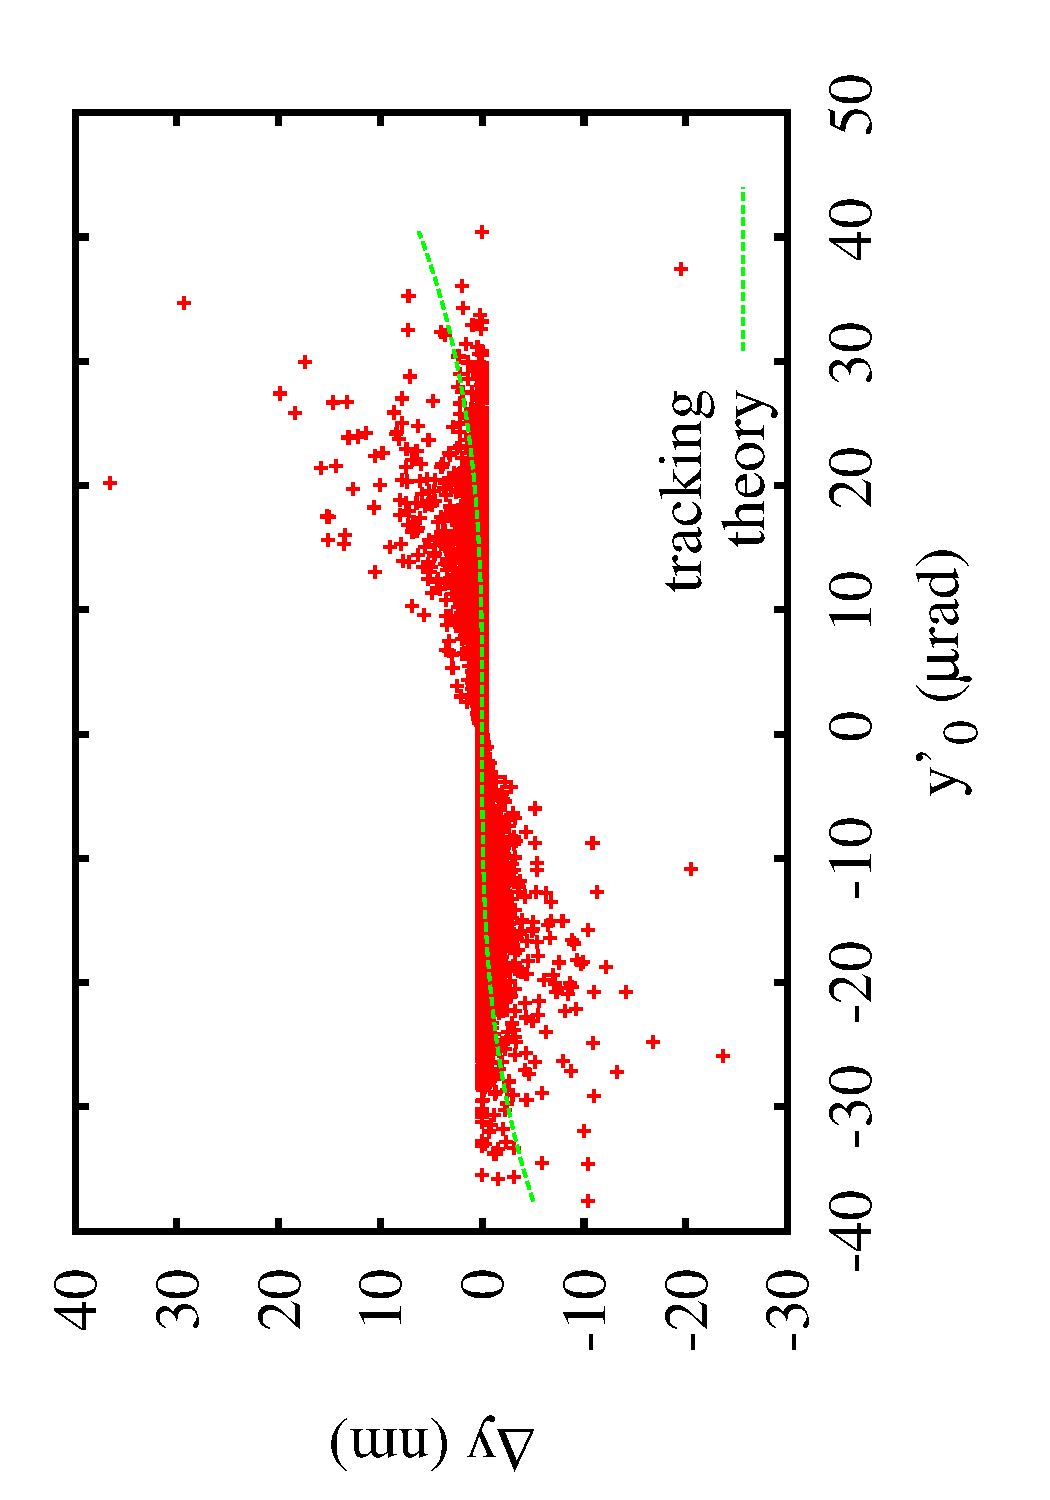
\includegraphics[scale=0.3,angle=-90]{plotdyrad.pdf}\caption{Correlation between the phase space coordinates $\Delta y,y'$ for CLIC 3 TeV from particle tracking and theoretical expression in Eq. (\ref{eq:deltamean}).}\label{f:correlation}
\end{figure}
This correlation could be removed from the beam size by a set of octupolar correctors to be presented in next Section.
\subsubsection{Correctors}
A pair of correctors, placed as in Fig. \ref{f:corrector}, is added to the strong focusing in order to mitigate the radiation effect. Particles that did not radiate along QD0 receive kicks in C1 and C0 cancelling one another. However, the C1 and C0 kicks do not cancel for particles that did radiate, this difference is used to correct only the particles trajectory change due to radiation.\par
The procedure consists in scaning the best position and multipole gradient ($s,k_i$) for C0, and then set C1 at QD0 input to cancel the effect of C0. If two points with same $\beta_y/\beta_x$ ratio are chosen, then the mutual cancellation of C1 and C0 correctors is limited only by the phase advance between them \cite{PhysRevSTAB.8.104002} and angle dispersion in the general case. Figure \ref{f:betaratio} shows the horizontal and vertical $\beta$ functions for CLIC 3 TeV in FD region, and their ratio.\par
The equal $\beta_y/\beta_x$ ratio for C0 and C1 condition is difficult to fulfill because C0 should be too close to the IP. In addition, it will lead to correctors running at very high strengths perturbing the beam.\par
A second approach is to minimize the phase advance between correctors. Therefore they will be located on both faces of QD0. This has the advantage of correctors running at lower strengths thanks to large $\beta$ functions.\par
\begin{figure}[!htb]
\centering
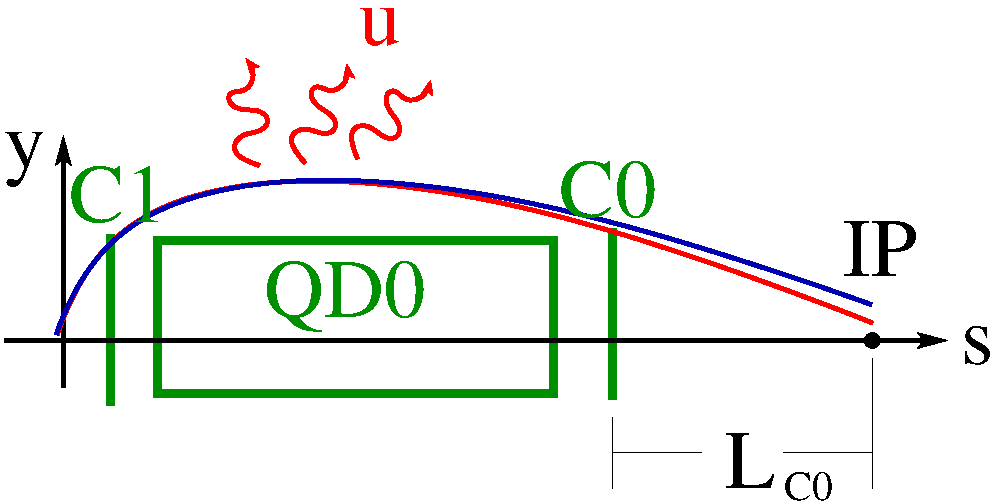
\includegraphics[scale=0.5,angle=0]{Oide2.pdf}\caption{For the nominal trajectory in blue, the kick in C1 must cancel the kick in C0. For all particles that radiate in red, the difference in kicks should cancel $\Delta y$.}\label{f:corrector}
\end{figure}
\begin{figure}[!htb]
\centering
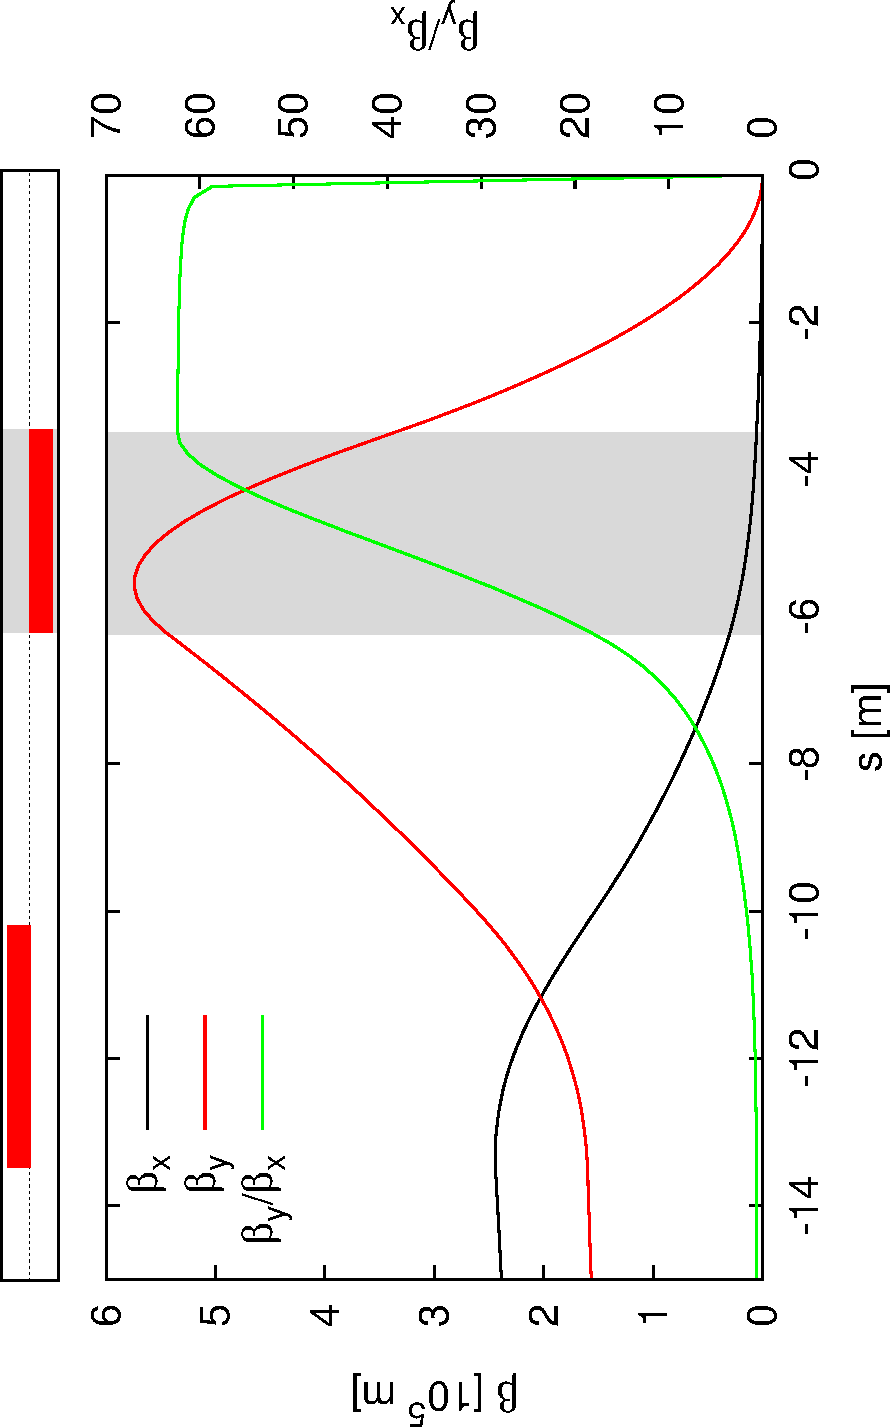
\includegraphics[scale=0.45,angle=-90]{lattice_CLIC_3TeVFD-crop.pdf}\caption{$\beta$ functions and $\beta_y/\beta_x$ ratio for CLIC 3 TeV FD, QF1 and QD0 in red on top. The dark area is occupied by QD0 and the IP is at $s=0$.}\label{f:betaratio}
\end{figure}
Two octupoles (OD0,OD1) were tried as correctors (C0,C1) to substract the cubic fit. A CLIC 3 TeV nominal beam with no energy spread is generated at the IP and tracked back to the entrance of the C1 without radiation with both correctors off. This beam is used to study the Oide effect mitigation in QD0 using correctors by tracking to the IP with radiation.\par
The best result obtained with the octupole correctors is a vertical beam size reduction by $(-4.3\pm0.2)$\% using OD0 only. Table \ref{t:correctors} shows the result of luminosity changes less than 10\% for the case with no radiation in QD0, with radiation, with one corrector and with the two correctors obtained with Guinea Pig ++ \cite{Schulte:382453}.\par
\begin{table}[!hbt]
\centering
\scriptsize
\begin{tabular}{c||c|c|c|c||c|c||c|c}\hline
& \multicolumn{2}{c|}{OD1} &\multicolumn{2}{c||}{OD0} & $\sigma_x$ & $\sigma_y$ & $L_{tot}$ & $L_{peak}$\\
& $L$ [m] & $k_3$ [m$^{-4}$] & $L$ [m] & $k_3$ [m$^{-4}$] &  [nm] & [nm] & \multicolumn{2}{c}{[$10^{34}$cm$^{-2}\cdot s^{-1}$]}\\\hline\hline
NO RAD & 0.01 & 0 & 0.01 & 0 & 47.45 & 0.69 & 7.7 & 2.9\\
RAD    & 0.01 & 0 & 0.01 & 0 & 47.45 & 1.18 & 7.5 & 2.7 \\
RAD    & 0.01 & 0 & 0.01 & -3900 & 47.45 & 1.13 & 7.4 & 2.7 \\
RAD    & 0.01 & 1502 & 0.01 & -3900 & 47.45 & 1.17 & 7.1 & 2.7 \\\hline
% NO RAD & 0.01 & 0 & 0.01 & -3900 & 47.42 & 0.77 & - & -\\
% NO RAD & 0.01 & 1502 & 0.01 & -3900 & 47.42 & 0.75 & - & -\\\hline
\end{tabular}\caption{Effect of octupolar correctors on the beam size, total luminosity and peak luminosity.}\label{t:correctors}
\end{table}
The Oide effect contribution to vertical beam size affects very little the luminosity. The single corrector option., OD0, does not show any improvement in peak luminosities. However, the case of two correctors OD1 and OD0 shows a drop in the total luminosity. This has been attributed to the limited cancellation between correctors due to different $\beta_y/\beta_x$ ratio and phase advance.\par
The possibility of slicing QD0 in two or three sections and mitigate the radiation effect with a pair of octupoles on each/any slice could be studied.\par
\subsection{Conclusions}
Radiation in the final quad sets a limit on the vertical beamsize, this is called Oide effect. Only for CLIC 3 TeV this limit is significant, therefore two possibilities have been explored to mitigate its contribution to beam size: double the length and reduce the QD0 gradient, or the integration of a pair of octupoles before and after QD0.\par
The best result with octupoles demonstrated vertical beam size reduction of $(4.3\pm0.2)$\%, with little or negative impact on luminosity. The correction scheme is currently limited by the phase advance and $\beta_y/\beta_x$ ratio between correctors. It may be possible to improve its performance by slicing QD0.\par

\newpage
%########################################################################
% Third part
%########################################################################
% \part{The Accelerator Test Facility (ATF/ATF2)}
\part{BPMs at the ATF2 Interaction Point (IPBPMs)}
\chapter{Relevance of ATF/ATF2}

\section{Facility purpose}
The main objective of the Accelerator Test Facility (ATF) built at the High Energy Accelerator Research Organization (KEK) in Tsukuba, Japan, is to serve as R\&D platform for the requirements of linear accelerators, in particular ILC. ATF obtained the record of minimum vertical beam emittance \cite{Kubo:2001ps,PhysRevLett.92.054802}, see Table \ref{t:ILC_ATF2param}, leading to the next step, the vertical beam size reduction at the IP.\par
The Final Focus Test Beam (FFTB) \cite{Berndt:1991ug}, at the Stanford Linear Accelerator Center (SLAC) in the  U.S.A., explored the beam size reduction using the non-local chromaticity correction scheme. It operated since 1994 to 1997 with a final result of 70nm in the vertical plane. The nominal 40~nm was not achieved and the difference was attributed to beam jitter and tuning limitations \cite{Araki1}.\par
The beam size reduction using the local chromaticity correction is explored by an extension of the original design, called ATF2 \cite{ATF2prop,grishanov:in2p3-00309474}, which involves an ILC-like FFS lattice scaled down to 100~m with two goals: ({\textbf{goal 1}) achieve 37~nm of vertical beam size at the IP and ({\textbf{goal 2}) the stabilization of the IP beam position at the level of few nanometres.\par
The CLIC, ILC and ATF2 main parameters are shown in Table \ref{t:ILC_ATF2param}, where the vertical chromaticity $\xi_y$ is similar for ATF2 and ILC designs. The ILC and ATF2 relative increase in beam size is a factor 10, calculated from $L^*$, $\beta^*$ and $\sigma_\delta$, if chromaticity is not corrected.\par
\begin{table}[hbt]
\centering
{\scriptsize
\begin{tabular}{l|c|c||c|c|c|c}\hline
Parameter & Symbol & Units &CLIC 3 TeV&CLIC 500 GeV& ILC & ATF2\\\hline\hline
Beam Energy per beam & $E$ & GeV & 3000 &250  &250 & 1.3 \\\hline
Energy Spread (e$^+$/e$^-$) & $\sigma_\delta$ & \% & 0.3 & 0.3 & 0.07/0.12 & 0.06$\sim$0.08\\\hline
Final quad to IP distance & $L^*$ & m & 3.5 & 4.3 &3.5/4.5\dag & 1.0\\\hline
Horizontal $\beta$ function at the IP & $\beta^*_x$ & mm & 6.9 & 9 &11 & 4\\\hline
Vertical $\beta$ function at the IP & $\beta^*_y$ & mm & 0.07 & 0.2 &0.48 & 0.1\\\hline
Normalized horizontal emittance & $\epsilon^*_{xN}$ & $\mu$m & 660 & 2400 & 10 & 2.8\\\hline
Normalized vertical emittance & $\epsilon^*_{yN}$ & nm & 20 & 25 & 35 & 31\\\hline
Horizontal beam size & $\sigma^*_y$ & nm & 45 & 200 & 5.9 & 37\\\hline
Vertical beam size & $\sigma^*_y$ & nm & 0.9 & 2.3 & 5.9 & 37\\\hline
Natural vertical chromaticity & $\xi_y$ & & 50000 & 43000 &7300/9400\dag & 10000\\\hline
\end{tabular}\caption{Design parameters of ILC and ATF2 Final Focus. \dag The ILC lattice has two detector options: SiD and ILD.}\label{t:ILC_ATF2param}
}
\end{table}\par
When compared with the current linear accelerator projects, ATF2 will not be as sensitive to time variations due to ground motion and wakefields, nor to misalignments, because the ATF2~FFS in an order of magnitude shorter than in ILC and because of the larger geometric emittances involved. However the tolerances to magnetic fields, jitter vibration and power supply stability are similar in ATF2 and ILC.\par
On the other side, ATF2 needs dedicated systems to measure the beam position and beam size at the IP because the focusing effects of beam-beam interactions used in a collider are not applicable.\par

\section{Beam line Description}
The ATF accelerator facility, shown in Fig.~\ref{f:ATF}, is composed of a photocathode giving electrons to a linac which accelerates the particles to 1.3~GeV, a damping ring to reduce the beam vertical and horizontal emittances and an extraction line which provides bunch packets to the Final Focus Section (FFS) where the beam is transported to the nominal IP and dump. The goal is to generate, accelerate and damp a train of 20 bunches with $2\times10^{10}$ particles per bunch and 2.8~ns bunch spacing. A detailed description is available in~\cite{ATF2prop,Alabau,Yves}.\par
\begin{figure}[htb]
\centering
\begin{subfigure}[b]{1.0\textwidth}
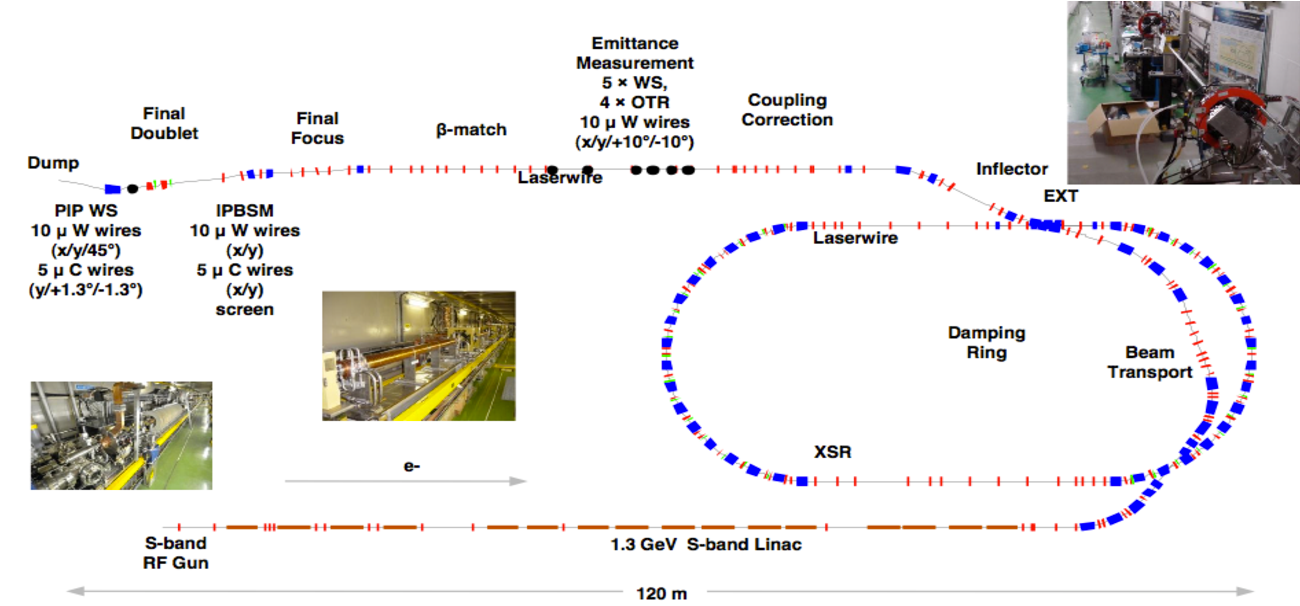
\includegraphics[angle=0,scale=0.70]{ATF-crop.pdf}\caption{Disposition of the Accelerator Test Facility (ATF), composed by a photocathode, a linac to 1.3GeV, a damping ring, an extraction line, the Final Focus (FF), and the beam dump.}\label{f:ATF_ATF2}
\end{subfigure}
\begin{subfigure}[b]{1.0\textwidth}
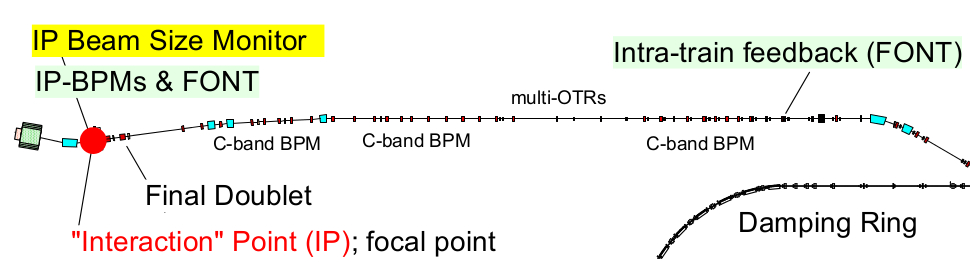
\includegraphics[angle=0,scale=0.65]{LigneATF2.jpg}\caption{Zoom over the extraction line, and Final Focus Section, highlighting the nominal Interaction Point location (IP). This region is known as ATF2.}\label{f:ATF2layout}
\end{subfigure}\caption{Diagrams containing the ATF composition and a zoom on the ATF2 section.}\label{f:ATF}
\end{figure}
\subsection{The RF Gun and Linac}
The total length of the linac is 80 m divided in: 18~m for the pre-injector section, a 70~m long accelerator section with energy compensation structures and 12~m for the transport line to the damping ring (DR) and a positron test stand.
The RF gun with a 1.6 cell S-Band Cs$_2$Te photocathode generates an electron beam with intensity up to 3.2nC per bunch. The pre-injector contains also an accelerating structure. An accelerating field of 35.2 MeV/m is required to accelerate 20 bunches of $2\times10^{10}$ particles per bunch. The linac is operated at a repetition rate of 25 pps (pulses per second) to allow circulating 5 bunch trains in the Damping ring. Table \ref{t:linac} shows the main parameters of the DR.
\begin{table}[hbt]
\centering
 \begin{tabular}{|c|c|}\hline
 Beam energy, $E_{beam}$& 1.54 GeV \\
 Bunch population, $N$& $2\times10^{10}$ \\
 Bunches per train, $N_b$ & 20 \\
 Bunch spacing, $\Delta t_{bunch}$ & 2.8 ns\\
 Energy spread Full Width, $\sigma_\delta$ & <1.0\% (90\% beam)\\
 Normalized emittance, $\epsilon_{Nx/y}$ & $< 3\times 10^{-4}$ m$\cdot$rad\\\hline
 \end{tabular}
 \caption{Basic design parameters of the ATF injector linac.}\label{t:linac}
\end{table}
\subsection{The Damping Ring}
The ring has a length of 138.6~m. It has achieved in 2004 a vertical normalized emittance of $1.5\times10^{-8}$ m$\cdot$rad, equivalent to $6$pm$\cdot$rad for a bunch intensity of $10^{10}$ particles. It was achieved by a precise alignment of components and beam control. The structure is a combination of bending magnets and wiggler cells where the value of the horizontal emittance is determined by the structure unit cell. The wigglers reduce the damping time and each bend is placed at the minimum of the dispersion in each periodic structure. The ATF DR consists in 36 of these units cells and the main parameters are in Table \ref{t:ATFDR}.
\begin{table}[hbt]
\centering
 \begin{tabular}{|c|c|}\hline
 Beam energy, $E_{beam}$& 1.54 GeV \\
 Bunch population, $N$& $2\times10^{10}$ \\
 Bunches per train, $N_b$ & 20 \\
 Bunch spacing, $\Delta t_{bunch}$ & 2.8 ns\\
 Energy spread Full Width, $\sigma_\delta$ & <1.0\% (90\% beam)\\
 Normalized emittance, $\epsilon_{Nx/y}$ & $3\times 10^{-6}/3\times 10^{-8}$ m$\cdot$rad\\\hline 
 \end{tabular}\caption{ATF DR main parameters.}\label{t:ATFDR}
\end{table}
\subsection{The extraction line}
In the extraction line the beam is extracted from the DR by means of a first kicker (KICKER1), and then passes off-axis through two quadrupoles centered on the DR reference orbit. Then, the beam passes through three septum magnets which complete the extraction. After the extraction, the beam passes through a dispersion supressor section to reduce fluctuations.\par
There are two extraction modes: single bunch and multibunch.\par
In single bunch mode one bunch is extracted approximately every 1/3 s from the damping ring to the ATF2 line. In multibunch mode a train of up to 20 bunches is extracted from the damping ring. The number of bunches and spacing are set by the damping ring fill up.\par
\subsection{The extraction diagnostic section}
After the extraction, the diagnostic section is used for measuring the emittance and dispersion ,and correcting betatron coupling. This section has been designed to be as close as possible to the ideal skew correction described in \cite{Woodley:453645}.\par
The measured vertical emittance in the diagnostic region downstream shows typically a factor 3~increase with respect to values obtained in the DR and dependence with beam intensity. One of the possibilities of the emittance growth is the non-linearity of the magnetic fields in the extraction region experienced by the beam when passing off-axis. One second possibility is the wakefields induced by the extraction kicker. The correlation with beam intensity is not fully understood; it could be due to the beam position monitors response.\par
Connecting dispersion and betatron matching plus careful alignment are the keys to mitigate the factor~3 increase in vertical emittance.\par
\subsection{The ATF2 lattice}
The ATF2 lattice can be subdivided in two sections : the matching section and the FFS. The following section describes the FFS.\par
% \subsubsection{The FFS}
The FFS focuses the beam to a small vertical beam size following the telescope design with local chromaticity correction, as in Sect. \ref{s:chromcorr}. The top of Fig.~\ref{f:FF_MADX} shows the lattice elements and the optics functions along the FFS. The Final Doublet (FD), QD0FF and QF1FF, provide the vertical and horizontal focusing, respectively. The horizontal off-momentum function $\eta$ and the pair of sextupoles in the FD are used to cancel the beam size dependence on energy spread at the IP.\par The second pair of sextupoles in the lattice section from 70~to~75~m are used to cancel the geometrical components induced by the sextupoles in the FD. And, additional chromaticity is created upstream QF7 to match the local correction~\cite{Raimondi:2000}, see Section \ref{s:chromcorr}.\par
\begin{figure}[htb]
 \vspace*{-1.5cm}
 \begin{picture}(0,0)
 \put(386,-76){\tiny IP}
 \put(372,-44){\tiny QD0}
 \put(354,-44){\tiny QF1}
 \put(198,-44){\tiny QF7}
%  \put(195,-43){\tiny IM}
%  \put(365,-76){\scriptsize FD}
 \put(70,-76){\scriptsize Matching Section}
 \put(220,-76){\scriptsize Final Focus Section (FFS)}
 \put(138,-286){\tikz\draw[blue,dashed,thick] (0,0) -- (0,8.42);}
%  \put(220,-30){\tikz\draw[red,dashed,thick] (0,0) circle (0.4);}
%  \put(-90,20){\hbar}
\end{picture}
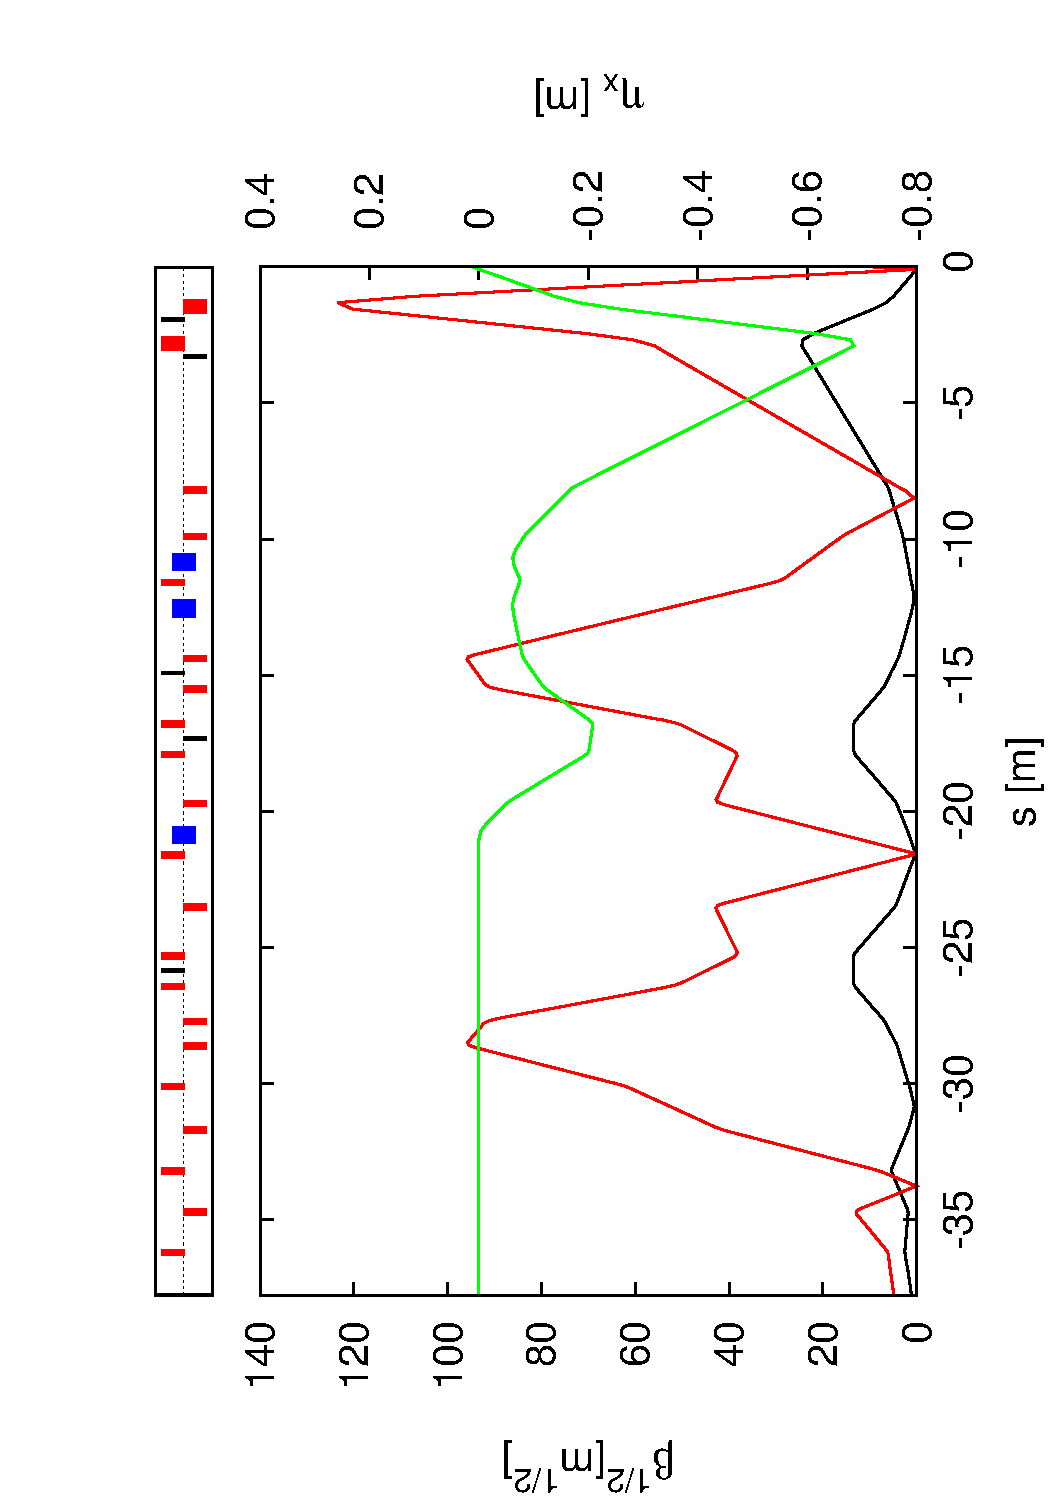
\includegraphics[angle=-90,scale=0.65]{lattice_ATF2_FF.pdf}\caption{Optical functions in the Final Focus Section at ATF2. On top is the ATF2 lattice: dipoles in blue, quadrupoles in red and sextupoles in black.}\label{f:FF_MADX}
\end{figure}
Quadrupole displacements are used to steer the beam, while sextupole displacements are used to induce corrective focusing (normal and skew components for horizontal and vertical displacements, respectively). This has an impact on the beam size. The tolerances to misalignments, roll angle and magnet strength errors in the FFS have been initially studied with a target of 2\% impact on the beam size, and it has resulted in similar tolerances as in ILC \cite{Yves}. 
All quadrupoles and sextupoles are placed on individual movers to allow the beam steering and adjustment of relative alignment in X, Y and Roll angle. 
\subsection{The IP Region}\label{s:opticsIP}
The $\beta$ functions at the IP, $\beta^*$, can be set by changing the matching section quadrupole strengths. Three configurations are normally used : 1BX1BY, 10BX1BY, and 100BX1000BY, where the factor indicates the number of times that the original $\beta^*$ has been amplified.\par
The 1BX1BY optics has the original design parameters. Here the angular divergence of the beam is $0.35$~mrad vertically and $0.52$~mrad horizontally in the IP region. \par
The 10BX1BY preserves the $\beta_y^*$ goal while relaxing the tolerance to multipole errors in magnets by increasing ten times the original $\beta_x^*$, making them comparable with those of ILC 500~GeV \cite{PhysRevSTAB.17.023501}. This optics is the one shown in Fig.~\ref{f:FF_MADX} and it is currently used in operation.\par
The 100BX1000BY optics sets a parallel beam through the IP area by enlarging the beam size at the IP. It is principally used to avoid the issues of large angle divergence displayed by the 1BX1BY optics.\par
Even smaller $\beta_y^*$ functions have been explored recently at ATF2 aiming to investigate resulting increases in tuning difficulty and beam size measurements limitations \cite{PateckiLowBeta}.\par
Figure \ref{f:BXYoptics} shows the beam size in vertical and horizontal planes for several optics combinations in a region of 300~mm around the IP. It also shows clearly how the beam divergence affects the beam size along the IP region.\par 
\begin{figure}[h]
 \begin{center}
 \hspace*{-1cm}
 \begin{subfigure}[b]{0.45\textwidth}
  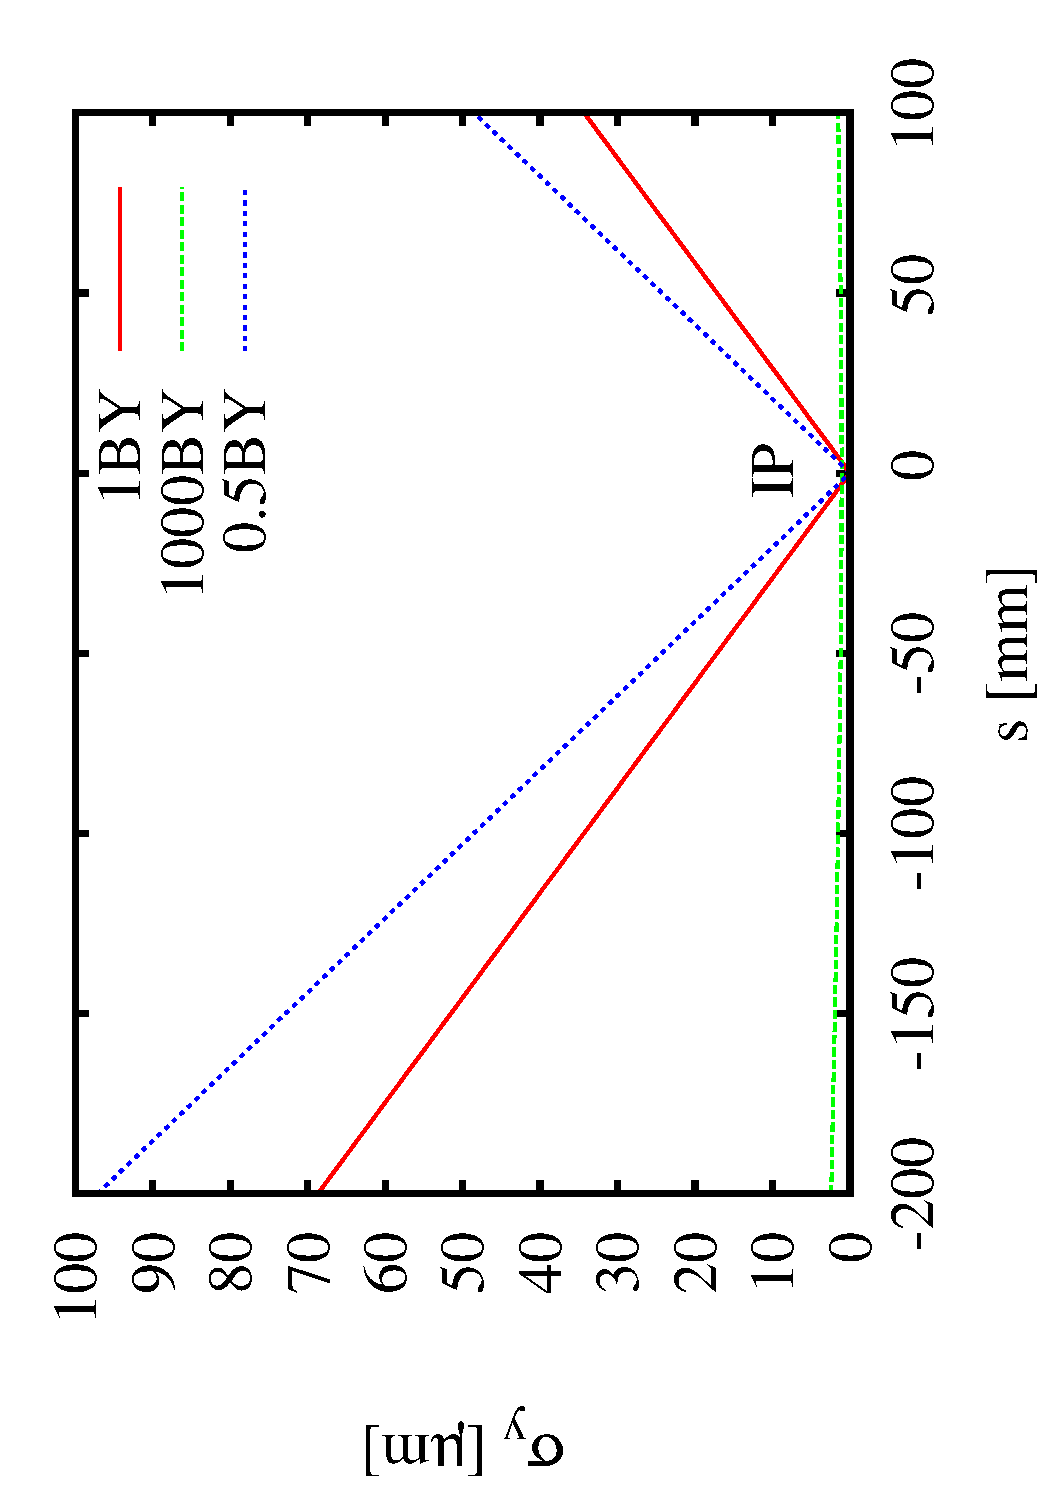
\includegraphics[angle=-90,scale=0.32]{optics_requ.pdf}\caption{Vertical beam size near the IP.}\label{f:opticsBY}
 \end{subfigure}\hspace{0.5cm}
\begin{subfigure}[b]{0.45\textwidth}
  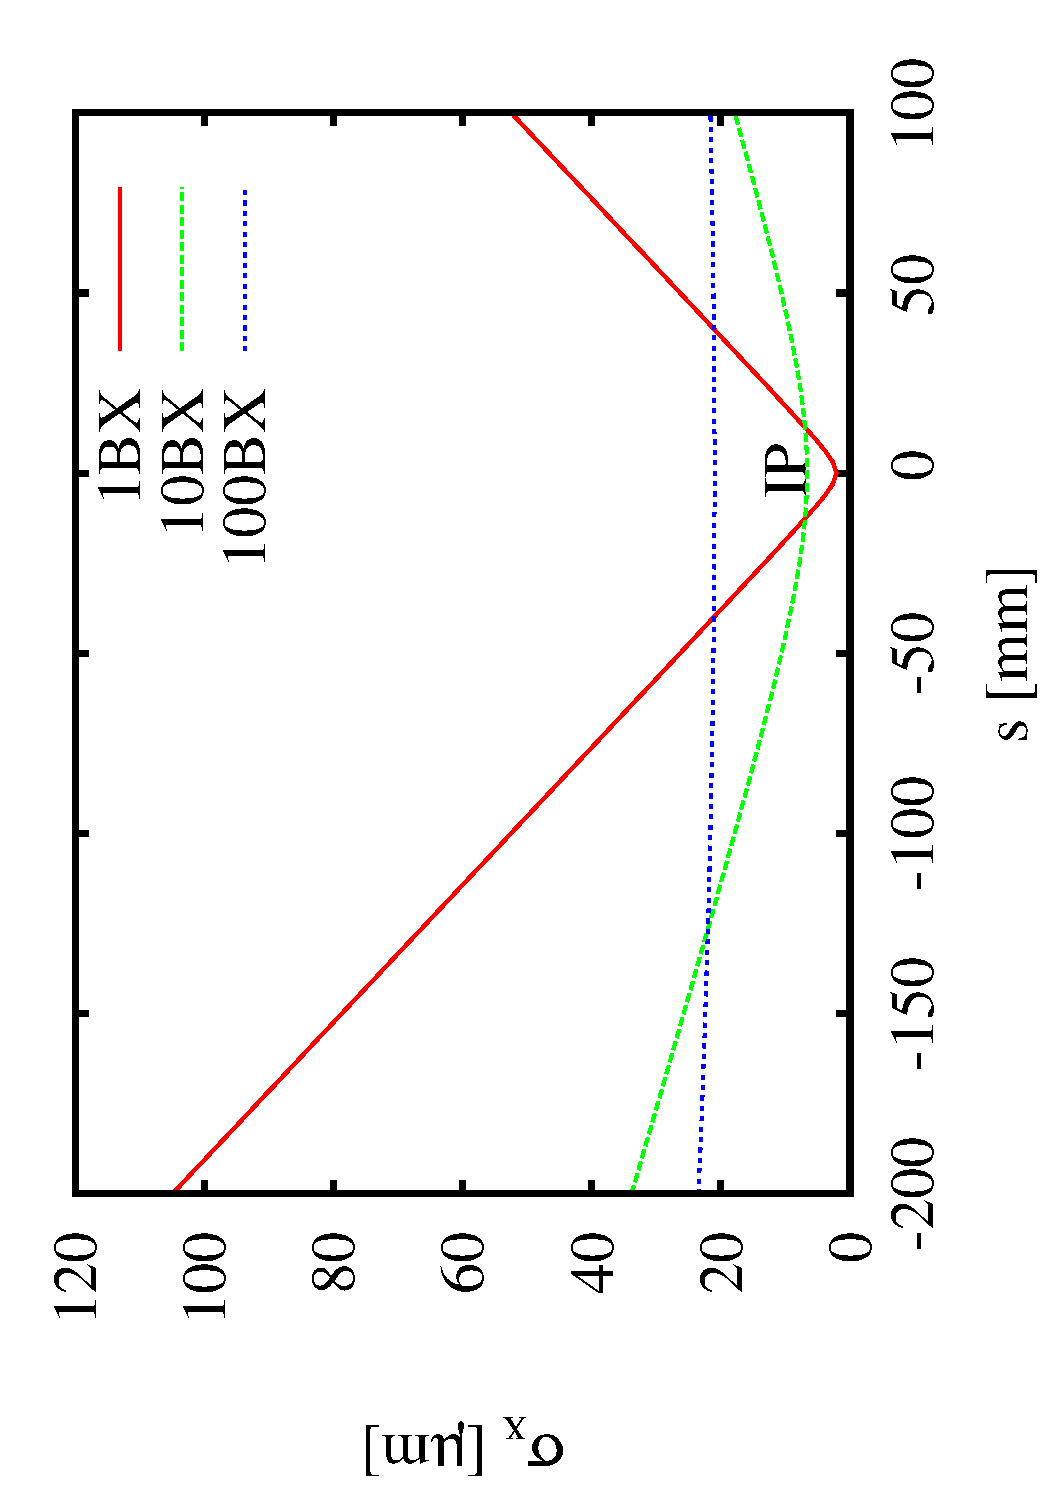
\includegraphics[angle=-90,scale=0.32]{optics_BX.pdf}\caption{Horizontal beam size near the IP.}\label{f:opticsBX}
 \end{subfigure}
  \caption{Vertical and horizontal beam sizes for 1BY, 1000BY, and 0.5BY in the vertical plane, and 1BX, 10BX and 100BX in the horizontal plane.}\label{f:BXYoptics}
 \end{center}
\end{figure}
The QD0 strength sets the vertical beam waist location with an small impact on the horizontal beam waist location, and viceversa for the QF1. The two are set to put the beam waist to its the nominal location at $s=0$. However, one or a combination of the two quadrupole strengths can be used to bring the beam waist to any location upstream or downstream. Moving the beam waist along the section of the IP region displayed in Fig.~\ref{f:BXYoptics} is effectively changing the focal distance by less than -20\% to +10\%.\par
QD0 and QF1 horizontal and vertical movers can also be used to steer the beam in the FD region, changing the position and angle through the IP region. Angles can also be steered by moving QF7 horizontally and vertically because of its location near a focal point upstream. See Fig. \ref{f:ATF2layout} showing the QF7 location and Eq. (\ref{eq:telescope}) to see that the kick at the input of a telescope lattice affects only the angle at the output.\par

\section{Beam Size Measurement at the IP}
A direct beam size measurement at the ATF2 IP is required because it can not be deduced from beam-beam effects as in a collider.\par
\begin{figure}[htb]
 \begin{center}
  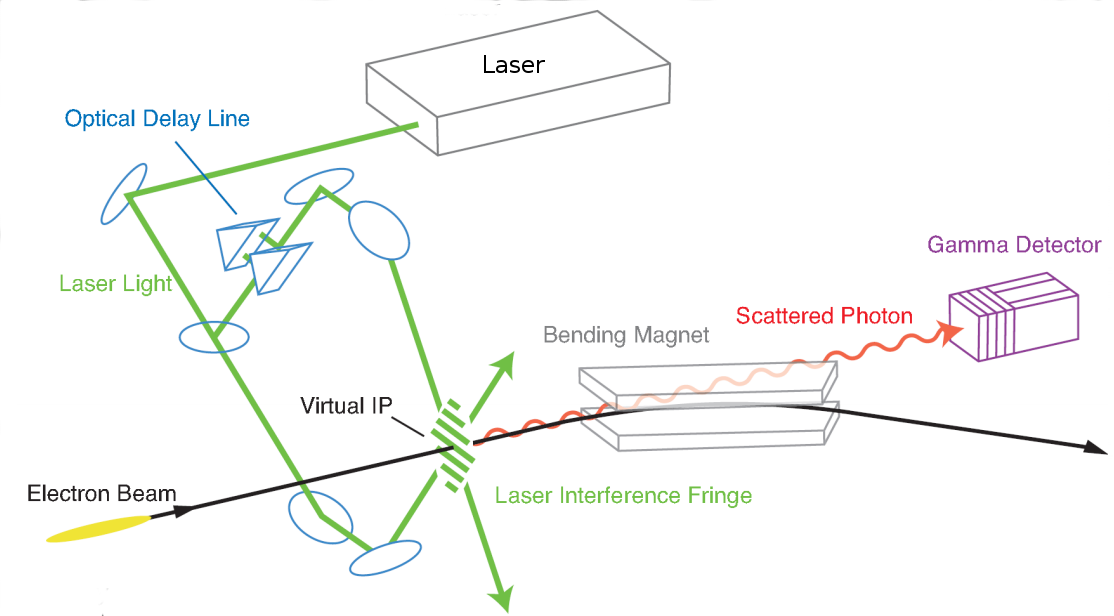
\includegraphics[angle=0,scale=0.5]{IPBSM_1.png}\caption{IPBSM schematic design. The particle beams cross the interference pattern generated by a perpendicular laser beam. The number of electron-photon interactions varies with the fringe size and the particle beam size.}\label{f:IPBSM}
 \end{center}
\end{figure}
The Beam Size Monitor (IPBSM) measures the number of scattered photons from an electron-photon collision between the particle bunch and a perpendicular interference pattern generated by high intensity laser perpendicular to the bunch trajectory \cite{Shintake1992453}. The number of photons is proportional to the photon density at the beam position. Moving the beam or scanning the phase of the laser fringe produces a modulation of gamma flux ray, the amplitude of which depends on beam size \cite{Yves}. Figure \ref{f:IPBSM} shows a schematic design of the IPBSM.\par
Such a device was previously used at the FFTB line at SLAC \cite{Shintake:1995sg}. A similar one is now located in the IP region at ATF2 \cite{Jackelinethese}.\par
\begin{figure}[htb]
 \begin{center}
  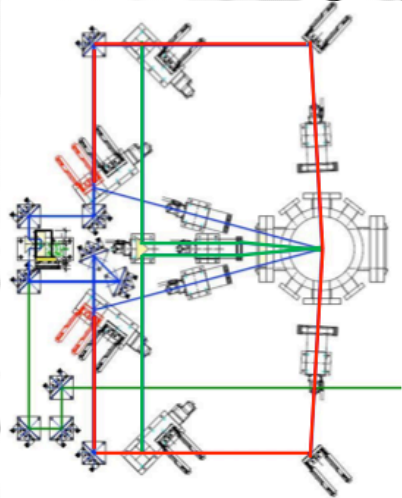
\includegraphics[angle=0,scale=0.35]{IPBSM_angles.png}
  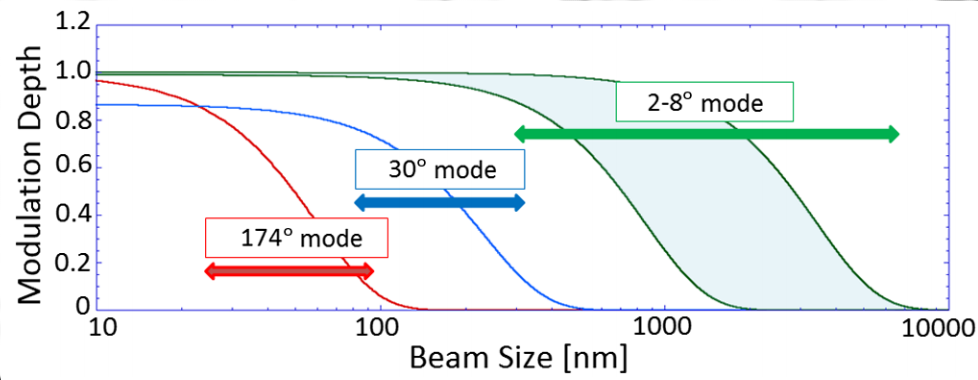
\includegraphics[angle=0,scale=0.455]{IPBSMreso.png}
  \caption{(Right) IPBSM laser path over the optical table perpendicular to the beam propagation. (Left) Beam size resolution for the angle modes : $2\sim8$\degree in green, 30\degree in blue and 174\degree in red.}\label{f:IPBSMangles}
 \end{center}
\end{figure}
At ATF2, it is installed on a vertical optical table where the laser incident angle can be adjusted to change the interference fringe pitch allowing measurements of beam sizes from 6~$\mu$m down to 25~nm. Figure \ref{f:IPBSMangles} shows the laser beam paths along the vertical optical table for three angle modes and the corresponding ranges of possible beam measurements.\par
Larger beam sizes are measured by a wire scanner installed in the same region. It consists in a wire moved across the beam generating bremsstrahlung gamma rays. The number of photons is proportional to the charge of the slice interacting with the wire at each position setting. Profiles are constructed from the number of photons as a function of wire position \cite{Hayano:2000xf}.

\section{Beam stabilization}
Three regimes are defined for the beam stability: random fluctuations over timescales which are effectively uncorrectable (jitter), fast varitions that can be corrected by feedback (FB) systems, and slow or static changes that can be addressed by systematic orbit correction (tuning).\par
The jitter requirement for goal 1 is beam jitter less than 30\% of $\sigma_y$, while goal 2 requires jitter less than 5\% of $\sigma_y$. The measured bunch position jitter upstream of the FD for single bunch extraction mode, i.e. the fluctuations on bunch position before the last strong focusing magnets, is around 10$\sim$20\% of beam size in the vertical plane and 5$\sim$10\% on the horizontal plane \cite{PateckiJitter}. Additional jitter could come from the mechanical vibration of the FD.\par
\subsection{Tuning}
The contribution to beam size due to field errors is considered static or slowly changing. It is possible to reduce their impact by systematic orbit correction using magnetic or mechanical means~\cite{ATF2prop}. Goal 1 jitter requirements can be achieved for single bunch extraction.\par
\subsection{Feedback}
The fluctuations coming from ground motion, magnet strength variations, changes in the damping ring, energy oscillations are considered fast errors. Aso, the bunch to bunch jitter from multibunch extraction requires active correction.\par 
The feedback system is then the last line of defense to correct the beam trajectory and three schemes are tested in ATF2 using two bunches.\par
\begin{itemize}
 \item Upstream FB: Measures the first bunch position in the IP region and uses a set of kickers upstream of the matching section to stabilize the position of the second bunch.
 \item Feedforward: Measures the first bunch position upstream of the matching section and uses a kicker in the IP region to stabilize the position of a second.
 \item Local IP FB: Measures the first bunch position in the IP region and uses a kicker in the IP region to stabilize the position of a second.
\end{itemize}

\section{Recent achievements and current work}
In 2014 vertical beam size about 55~nm was observed at ATF2 \cite{Kubo50nm}, and since then smaller beam size are achieved as a regular basis down to 44~nm \cite{KuboCLICws2015}, demonstrating the local chromaticity correction method at charges of about~$0.1\times10^{10}$ particules per bunch.\par
A main identified issue, intensity dependence, is currently explored by the ATF2 collaboration. Nonetheless, at low intensities, the beam size remains above the design 37~nm. Possible contributions are: (1) the increase of the incoming beam emittance along the ATF2 line, (2) systematic errors and resolution limitations on the beam size monitor, (3) beam drift/jitter beyond the tolerable margin and  (4) undetected optics mismatch.\par
Last two issues can be adressed by measuring the beam trajectory in the IP Region after the Final Doublet. In addition, looking forward to \textbf{goal 2}, beam position measurement is a requirement for beam stabilization.\par
The work here described corresponds to the beam position monitors installed in 2013 by LAL in collaboration with Kyungpook National University (KNU), the Feedback in Nanosecond Timescale (FONT) group from Oxford, and the ATF2 staff.\par

\section{Position Measurement Requirements}
A direct beam position measurement at the ATF2 IP is required because it can~not be deduced from beam-beam focusing effects as in a collider \cite{Bambade:1989pb}.\par
Knowing the beam trajectory with nanometric precision is valuable information for beam tuning and a requirement for feedback. The position measurement system could be used to correct the beam positions used in the reconstruction of the IPBSM modulation pattern, in order to remove the dilution from beam jitter in the beam size reconstruction pulse by pulse.\par
Therefore, a set of three cavities (IPA, IPB and IPC), two upstream and one downstream of the nominal IP, were installed and are used to measure the beam trajectory in the IP region, thus providing enough information to reconstruct the bunch position and angle at the IP.\par
Cavities are located at $s=-167.9$ mm, $s=-87.1$ mm and $s=87.1$ mm, with respect to the nominal IP at $s=0$. It has been shown in section \ref{s:opticsIP} the effect of different optics on the beam size along the IP region. As the measured beam jitter upstream is around $10\sim20$\% of beam size, then, the change of optics will have a direct impact on the dynamic range of the position measurement.\par %The following subsections give an estimation of the beam jitter.\par
% \subsubsection{Beam waist at one cavity using 1BX1BY and 10BX1BY optics}
\subsubsection{Dynamic Range}
Table \ref{t:sigmacavities1000BY} shows that beam size only increases by a factor two among the cavities using the 1000BY optics, while Table \ref{t:sigmacavities1BY} shows a beam one and two thousand times larger than the beam size at the focal point, due to the large divergence in the nominal optics.\par
From these optics settings the maximum vertical beam size is 58~$\mu$m. The dynamic range required for the cavity is then around 10~to~11~$\mu$m using the 20\% jitter to beam size ratio.
\begin{table}[h]
 \centering
\begin{tabular}{c||c|c|c|c}\hline
  & IPA & IPB & IP & IPC\\\hline\hline
  $s$ [mm]& -174.2 & -87.1 & 0 & 87.1 \\\hline
  $\sigma_y$ [1.086$\mu$m]&2.0&1.3&1&1.3\\\hline
  $\sigma_{y'}[0.011$mrad]&0.5&0.8&1&0.8\\\hline
\end{tabular}\caption{Vertical beam size at the cavities positions and the IP with the 1000BY optics.}\label{t:sigmacavities1000BY}
\end{table}
\begin{table}[h]
 \centering
\begin{tabular}{c||c|c|c|c}\hline
  & IPA & IPB & IP & IPC\\\hline\hline
  $s$ [mm] & -174.2 & -87.1 & 0 & 87.1\\\hline
  $\sigma_y$ [34~nm]&$1.7\times10^3$&871&1&871\\\hline
  $\sigma_{y'}$ [0.3~mrad]&$0.6(10^{-3})$&$1.2(10^{-3})$&1&$1.2(10^{-3})$\\\hline
\end{tabular}\caption{Vertical beam size at the cavities positions and the IP with the 1BY optics.}\label{t:sigmacavities1BY}
\end{table}
\subsubsection{Resolution and Calibration}
The beam stabilization to the nanometer level requires position measurement with nanometric resolution. In addition, due to the low $\beta^*$ for the nominal 1BX1BY optics, the beam size and therefore the jitter increases rapidly making the 1~nm resolution over the 10~$\mu$m dynamic range a challenge. The calibrations must be then valid for measurement over 3 to 4 order of magnitude.\par

% \chapter{Beam Position Monitor Requirements}
\section{Beam size monitoring Compatibility}
The Beam Size Monitor (IPBSM) measures the scattered photons from an electron-photon collission between the particle bunch and a perpendicular interference pattern generated by high intensity laser perpendicular to the bunch trajectory \cite{Shintake1992453}. Fig. (\ref{f:IPBSM}) shows an schematic design of the IPBSM.
\begin{figure}[htb]
 \begin{center}
  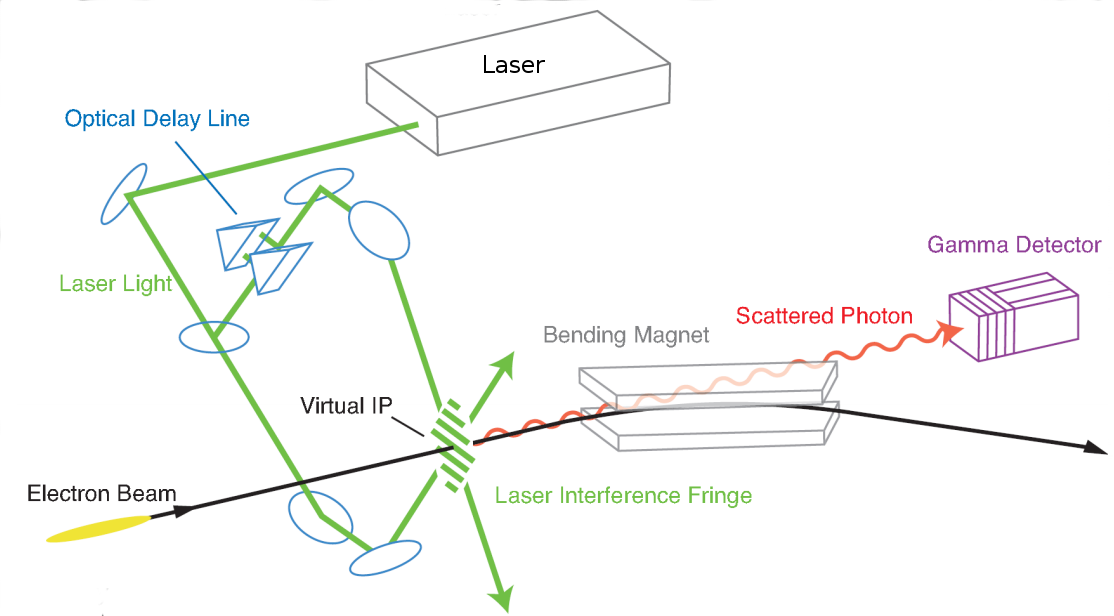
\includegraphics[angle=0,scale=0.5]{IPBSM_1.png}\caption{IPBSM schematic design. The particle beams crosses the interference pattern generated by a perpendicular beam. The number of electron-photon interactions varies with the fringe size and the particle beam size.}\label{f:IPBSM}
 \end{center}
\end{figure}
The current IPBSM at ATF2 \cite{Jackelinethese} is installed in a vertical optical table where the laser incident angle can be adjusted to change the interference fringe size giving four orders of magnitude of beam size resolution. Fig. (\ref{f:IPBSMangles}) shows the beam path along the vertical optical table for three angles modes and the correspoding range of beam measurements.\par
\begin{figure}[htb]
 \begin{center}
  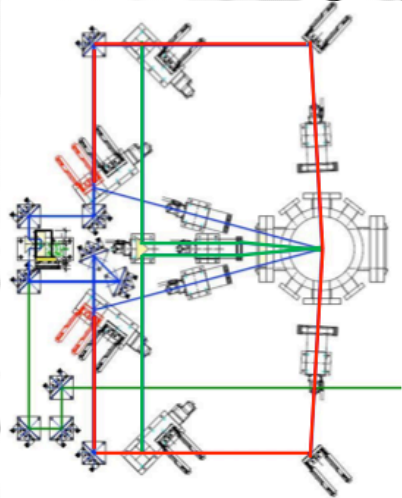
\includegraphics[angle=0,scale=0.35]{IPBSM_angles.png}
  \includegraphics[angle=0,scale=0.455]{IPBSMreso.png}
  \caption{IPBSM laser path and beam size resolution for the angle modes : $2\sim8$\degree in green, 30\degree in blue and 174\degree in red.}\label{f:IPBSMangles}
 \end{center}
\end{figure}
The beam positioning system should not interfere with the IPBSM measurements. Therefore, mechanical dimensions and weight should be restricted to those supported by the vertical optical table. This will allow to have a common reference point between the two structures.\par 
In addition, the longitudinal direction must be set to match the lattice IP position, the IPBSM IP and the beam position monitor in a common region. A tolerance of several cm could be of great advantage due to the dimensions and apertures of the optical components in the laser path.\par
Synchronization between the beam position monitor data and the IPBSM data would allow to mitigate the effect of large beam fluctuations on beam size measurement by discarding trajectories too far from the IPBSM best resolution spot.\par
\section{Optics in the IP Region}
The $\beta^*$ functions at the IP can be set by changing the upstream magnets strength. Three configurations are normally used : 1BX1BY, 10BX1BY, and 100BX1000BY, where the factor indicates the number of times that the original $\beta^*$ has been amplified.\par
The 1BX1BY optics has the original design parameters. Here the angular divergence of the beam is $0.35$mrad vertically and $0.52$mrad horizontally in the IP region. \par
The 10BX1BY preserves the $\beta_y^*$ goal while relaxing the tolerance to multipole errors in magnets by increasing ten times the original $\beta_x^*$, making them comparable with those of ILC 500GeV \cite{PhysRevSTAB.17.023501}. This optics has been plot in Fig. (\ref{f:FF_MADX}) and it is currently used in operation.\par
The 100BX1000BY optics sets a parallel beam through the IP area, principally used to avoid the issues of large angle divergence displayed by the 1BX1BY optics.\par
Even smaller $\beta_y^*$ functions have been explored recently at ATF2 aiming to estimate lower $\beta^*$ tunability and IPBSM limitations \cite{PateckiLowBeta}.\par
Figure (\ref{f:BXYoptics}) shows the beam size in vertical and horizontal plane for several optics combinations in a region of several cm around the IP. It also shows clearly how the beam divergence affects the beam size along the IP region. Now, considering the measurement of beam position, it has been shown by previous measurement results that beam jitter upstream the FD is around 10$\sim$20\% of beam size on the vertical plane and 5$\sim$10\% on the horizontal plane \cite{PateckiJitter}. 
\begin{figure}[htb]
 \begin{center}
 \hspace*{-1cm}
 \begin{subfigure}[b]{0.45\textwidth}
  \includegraphics[angle=-90,scale=0.32]{optics_requ.pdf}\caption{Vertical beam size near the IP.}\label{f:opticsBY}
 \end{subfigure}\hspace{0.5cm}
\begin{subfigure}[b]{0.45\textwidth}
  \includegraphics[angle=-90,scale=0.32]{optics_BX.pdf}\caption{Horizontal beam size near the IP.}\label{f:opticsBX}
 \end{subfigure}
  \caption{Vertical and horizontal beam sizes for 1BY, 1000BY, and 0.5BY in the vertical plane, and 1BX, 10BX and 100BX in the horizontal plane.}\label{f:BXYoptics}
 \end{center}
\end{figure}
If the jitter to beam size proportion is preserved in the FD and IP region, then, a minimum dynamic range between $5\sim10\mu$m is required for vertical position measurement with the previously mentioned optics and 10\% jitter. While the horizontal plane dynamic range must be close to $10\mu$m.\par
Having in mind the stabilization of the beam trajectory at the IP by few nanometers, it is clear that beam monitoring system must have a resolution equal or better than this. This implyes the big requirement of $10^{-4}$ resolution, linearity and stability over the entire dynamic range.\par
Knowing the beam trajectory with this precision is valuable information for beam tuning that could bring the beam jitter down, relaxing the dynamic range/resolution requirements, including the identification of local jitter sources in the FD and IP region.\par
\section{Feedback}
Under the goal 2 scope, the beam stabilization must be operative in different configurations : intra-train targeting pulse to pulse measurement and correction, inter-train stabilization targeting the train to train measurement and correction, both relying in the correlation measurement and correction in several scales of time.\par
Probably the most direct type is an intra-train active stabilization by feedback in the IP region. It consist in the measurement of a first bunch trajectory to correct the second and following. This avoids the propagation to upstream correctors and reduces the time latency restriction for the processing electronics determined by the time between pulses at maximum.\par
The ILC and CLIC colliders differ largely in this parameter : 0.5ns for CLIC and 367ns for ILC. The minimum bunch spacing at ATF is 2.8ns \cite{ATF2prop,BurrowsIntraTrain}, therefore it can not test CLIC specifications. However, in single-bunch mode, a maximum of three bunches with 154ns spacing are stored in the damping ring and can be used to test the intra-train feedback conceived by FONT \cite{BurrowsIntraTrain2,BurrowsIntraTrain3}.\par
The beam position monitor response and processing electronics latency must remain inside the tolerable values to perform feedback between two bunches.\par

\chapter{BPMs System description}
In this section I describe the beam position monitor (BPM) system installed at the IP region and the signals analysis method used test the system.\par
\section{The system}
The system consist in three cavities inside a vacuum chamber shown in Fig. \ref{f:vacuumchamberdes} which is fixed to the optical table used for the IPBSM laser and optical instruments. Flanges and viewports on the sides are compatible with the IPBSM operation. Inside the chamber, a system of three cavities (IPA, IPB and IPC) are installed in two separated blocks: one block upstream for IPA and IPB and the other downstream the IP for IPC.\par
Each block is placed over a piezo-electric displacement system shown in Fig. \ref{f:piezosystem} with three degrees of freedom: vertical displacement, horizontal displacement and pitch angle. Position and angle conventions can be seen in Annex \ref{s:BPMscoord}. \par
\begin{figure}[htb]
\centering
\begin{subfigure}{0.4\textwidth}
 \includegraphics[scale=0.28]{chambrevide.jpg}\caption{Vacuum chamber design.}\label{f:vacuumchamberdes}
\end{subfigure}
\begin{subfigure}{0.5\textwidth}
 \includegraphics[scale=0.3]{BPMs01.jpg}\caption{Piezo-electric displacement system and cavities.}\label{f:piezosystem}
\end{subfigure}
\end{figure}
This piezo mover system is remotely controlled to align the cavities with the beam, and to do systematic studies of the cavity sensitivity to position change. A set of in-vacuum PT100 thermal gauges are included on each block. The initial checkings on the system can be consulted in \cite{Bambade2013}, and the control and readout scheme can be seen in Annex \ref{s:annexB} with alignment results.\par
\subsection{The cavities}
Cavities for beam position measurement show good stability since precision depends on mechanical precision. Resolution of thermal noise level can be achieved by narrowing the dynamic range and using high gain electronics since signal is small near the cavity center. The following is a description of the cavity parameters as presented by Nakamura in \cite{Nakathese}.\par
\subsubsection{Cavity modes}
The cavity consists of a cavity and a waveguide. When the particles passes the cavity, it resonates in several modes at frequencies given by the cavity dimension and shape \cite{PhysRevSTAB.15.042801}.\par 
Cilyndrical coordinates are used for cilyndrical cavities. The electric $E=(E_r,E_\phi,E_z)$ and magnetic field $B=(B_r,B_\phi,B_z)$ are excited in the cavity. For beam position monitoring TM $B=(B_r,B_\phi,0)$ is essential. Three numbers $m,n,l$ which are the node numbers in $r,\phi,z$ are used to identify the nodes. The TM$_{010}$ is the monopole mode and it is used for charge intensity measurement and downmixing of the signals from the position sensitive cavities. It is shown in Fig. \ref{f:monopole}.\par
In a similar way, rectangular coordinates are used for rectangular cavities. The electric $E=(E_x,E_y,E_z)$ and magnetic field $B=(B_x,B_y,B_z)$ are excited in the cavity. For beam position monitoring TM $B=(B_x,B_y,0)$ is essential. Three numbers $m,n,l$ which are the node numbers in $x,y,z$ are used to identify the nodes. The TM$_{120}$ and TM$_{210}$ are the dipole modes and are used for bunch position measurement. The TM$_{110}$ is monopole mode in rectangular cavities. They are shown in Fig. \ref{f:dipole}.\par
\begin{figure}[htb]
\centering
\includegraphics[scale=0.4]{TMdipole.jpg}.\caption{Dipolar and monopolar mode in rectangular cavities.}\label{f:dipole}
\end{figure}
\begin{figure}[htb]
\centering
\includegraphics[scale=0.4]{TMmonopole.jpg}.\caption{Monopolar mode in cilindrical cavities.}\label{f:monopole}
\end{figure}
Only the dipole mode is of interest for beam position measurement so it is separated from other modes which are considered noise components. The separation between the vertical and horizontal dipole mode is made by making the cavity rectangular, giving different the resonant frequencies per plane.\par
A set of slots is done on the cavities to couple only the dipole mode to a waveguide with a cut-off frequency above the monopole mode. This is made to separated the dipole signal from large noise comming from the monopole component. An antenna pick-up the signal at the waveguide and connects it to the output port. The cavity design has then four ports, two ports in antiphase per plane, one on each side. Figure \ref{f:waveguide} shows the cavity transversal plane with the four slots and the coupling to the waveguide and the antena for the horizontal ports.\par
\begin{figure}[htb]
\centering
\includegraphics[scale=0.4]{Waveguide.jpg}.\caption{Coupling to the dipole mode of the cavity.}\label{f:waveguide}
\end{figure}
\subsubsection{Output signal}
Voltage of a resonant mode excited at a cavity by passing beam, $V_{exc}$, is represented as
\begin{equation}
 V_{exc}=\frac{\omega}{2}\left(\frac{R}{Q}\right)q
\end{equation}
where $\omega$ is resonant angular frequency of the mode, and $q$ is the beam charge, and $R$ is the shunt impedance and $Q$ is the quality factor which represents the efficiency of the resonant mode of a cavity. The factor $R/Q$ is
\begin{equation}
 \frac{R}{Q}=\frac{|\int E\cdot ds|^2}{\omega U}
\end{equation}
where $U$ is the energy stored in the cavity and $E\cdot ds$ is the longitudinal component of the electric field in the cavity generated by the passing beam. The cavity design for the IP region targets high $R/Q$ (high $Q_0$), minimizing the energy loss in cavity walls and maximizing the output power.\par
The effect of bunch length $\sigma_z$ is an effective reduction of $V_{exc}$ given by the expression
\begin{equation}
 V_{totalexc}=V_{exc}\exp\left(-\frac{\omega^2\sigma_z^2}{c^2}\right)
\end{equation}
The stored energy of a cavity is $U=V_{totalexc}^2/(\omega R/Q)$, and the output power is $P_o=\omega U/Q_{ext}$, where $Q_{ext}$ is the quality factor of the external coupling. Detecting the power output, $P_o$, by an impedance $Z$ gives the output voltage
\begin{equation}
 V_{out0}=\sqrt{ZP_{o}}=\frac{wq}{2}\sqrt{\frac{Z}{Q_{ext}}\frac{R}{Q}}\exp\left(-\frac{\omega^2\sigma_z^2}{2c^2}\right)
\end{equation}
% \subsubsection{Decay time}
The energy disipation in the cavity is
\begin{equation}
 U=U_0 e^{-\frac{\omega}{Q_L}t}
\end{equation}
where $\frac{1}{Q_L}=\frac{1}{Q_0}+\frac{1}{Q_{ext}}$, and energy decay time $\tau=Q_L/\omega$. As the signal is proportional to the square root of the power, then the signal decay time is a factor two smaller.\par
Finally, as the $R/Q$ factor depends on the longitudinal component of the electric field, the integration depends on the TM mode. It has been derived by \cite{Nakathese} concluding that in the dipole mode $R/Q$ depends on the square of the bunch transverse position in the case of bunch passing near the center, and the monopole mode $R/Q$ is independent of position. From this, the output voltage in the TM$_{120}$ and TM$_{210}$ is proportional to position, while TM$_{110}$ and TM$_{010}$ are not.\par
\subsubsection{Components orthogonal to position}
Additional components are present in the cavity signal output which are orthogonal to bunch position. They have been described by \cite{Nakathese} as
\begin{equation}
 V=V_{position}+iV_{angle}+iV_{tilt}+iV_{commontail}
\end{equation}
where the $i$ shows a $\pi/2$ phase difference, and the following is a brief description of the components:\par
\begin{itemize}
 \item Angle: a cavity of length $L$ gives a position voltage as $V_{position}=Ax\sqrt{L}\sin(\omega t)$. Assuming a beam passing through the cavity center making an angle $x'$, it can be decomposed in the sum of two position signals with $x=x'L/4$ and phase difference of $\pm L/4c$, affecting the amplitude by $\sin(\omega L/4c)$ and phase by $\pi/2$. The ratio of angle to position signals for $\omega L/4c\ll 1$ is
 \begin{equation}
  \frac{|V_{angle}|}{|V_{pos}|}=\frac{\omega L^2}{2\sqrt{2}c}\frac{x'}{x}
 \end{equation}
\item Tilt: a cavity gives a position voltage as $V_{position}=Aqx\sin(\omega t)$. The beam is decomposed in two point with $q/2$ total charge each, while traversing the cavity with an angle $\theta$. The sum of two position signals with $q/2$ charge each,  $x=\sigma_z\theta$ being $\sigma_z$ the bunch charge, and phase difference of $\pm\sigma_z/c$ will affect the amplitud by $\theta\sigma_z^2/c$ and phase by $\pi/2$. The ratio of angle to position signals is
\begin{equation}
  \frac{|V_{tilt}|}{|V_{pos}|}=\frac{\omega \sigma_z^2}{c}\frac{\theta}{x}
\end{equation}
\item Commontail: the common-tail \cite{Shintake:1998fga} comes from the monopole component. At the dipole component frequency it is 2 to 3 orders of magnitude stronger that the dipole component. However, it is attenuated by the coupling to the waveguide. Nakamura \cite{Nakathese} shows that the phase advance between the monopole and the dipole signals is $\pi/2$.\par
\end{itemize}
The phase difference of these components allow one to remove them from the position signal by phase detection. In addition the cavity design was conceived to reduce the angle signal because of the large beam divergence seen in Sect. \ref{s:opticsIP}.\par
\subsubsection{Cavities at the IP Region}\label{s:IPBPMsignals}
The three cavities (IPA, IPB and IPC) are rectangular and resonate in the TM$_{210}$ mode at 5.7 GHz in the horizontal plane and TM$_{120}$ at 6.4 GHz in the vertical plane. They have a design decay time of 19~ns (horizontal) and 17~nm (vertical), and sensitivities to bunch position of 2.2~$\mu$V/nm/nC (horizontal) and 3.7~$\mu$V/nm/nC (vertical). Two additional cilyndrical cavities with decay time of 29~ns, sensitivity to bunch charge of 3.27V/nC, one per resonant frequency, are placed downstream of the IP to measure the bunch charge and to downmix the C-Band frequency signals; these are the reference cavities.\par
The IPA, IPB and IPC sensitivity to orthogonal components are: position to angle ratio of 3.2~$\mu$m/mrad, position to bunch tilt  ratio of 8.6~$\mu$m/mrad with $\sigma_z$=8~mm and unknown commontail component.\par
Previous to the installation, the cavity signals decay time was measured giving the results shown in Table \ref{t:decayt}. In particular IPC shows a shorter signal than IPA and IPB. The effect of the large difference between the design and the measured values on resolution is under investigation.\par
\begin{table}[h]
\centering
\begin{tabular}{c|c||c|c|c}\hline
 Plane & Design & IPA & IPB & IPC \\\hline\hline
  X [ns] & 19.41 & 8.722 & 8.181 & 4.925\\
  Y [ns] & 17.49 & 11.11 & 11.25 & 6.745\\\hline
\end{tabular}\caption{Measured decay time for the three cavities before installation.}\label{t:decayt}
\end{table}
The measured resonant dipole frequency and the design show good agreement in Table \ref{t:dipolefreq}.
\begin{table}[h]
\centering
\begin{tabular}{c|c||c|c|c|c}\hline
 Plane & Design & Average & IPA & IPB & IPC \\\hline\hline
  X [MHz] & 5712 & 5712 & -2 & -2.5 & +2.5\\
  Y [MHz] & 6426 & 6420 & +1 & 0 & -3.5\\\hline
\end{tabular}\caption{Resonant dipole frequency measurement at KEK before installation.}\label{t:dipolefreq}
\end{table}

\subsection{The processing electronics}\label{s:processing}
Each position measurement cavity has two output ports in antiphase per plane connected to independent processing electronics  to downmix the signals, separate them into two orthogonal components called $I$ and $Q$, and set the gain according to beam charge conditions. A set of remotely-controllable attenuators, variable between 0-70 dB in steps of 10 dB is used to increase the linear range of electronics at the expense of resolution.\par
At the moment the reference cavities are not used to downmix the position cavities signals directly to base band. Instead a 714~MHz signal from the DR is used to downmix the three to 714~MHz in a first stage and then a second stage downmixes the position cavities to baseband using the reference cavity signal. This allows the installation of the second stage outside the ATF2 line, aiming the study of the signal with different phase detection setting changed by hand in hardware. An scheme of the electronics is in Fig. \ref{f:elect}. The following is a description of components extracted from \cite{Nakathese}.\par
\begin{figure}[htb]
 \centering\hspace*{-1cm}
 \includegraphics[scale=0.7,angle=-90]{Electr-crop.pdf}\caption{Processing electronics per BPM per plane.}\label{f:elect}
\end{figure}
\begin{itemize}
 \item Combiner: The combiner outputs the difference of the signals. However, the signal from the two cavity ports are in antiphase so the net effect is factor 2 of amplification.\par
 \item Variable attenuator: it attenuates the input signal from 0~dB to 70~dB in steps of 10~dB. The purpose is to enlarge dynamic range at the expense of resolution.\par
 \item First stage of down conversion: it downmixes the BPM and reference cavity signals to 714~MHz using an $8\times714$~MHz signal from the LOCKED LO module, and amplifies the output by 20~dB. It is required to do it as close as possible to the BPMs because of the short decay time.\par
 \item LOCKED LO: Multiplies the frequency of the DR 714~MHz by a factor 8 to perform the first stage of signal downmixing.\par
 \item Limiter detector: Set a constant amplitud of the Reference signal at 714~MHz to be used for the downmixing in the second stage. Fig. \ref{f:detector} shows a diagram with 4 outputs to be used for downmixing. It also outputs the signal proportional to charge.\par
 \item Phase detector: It sets the common phase between the ref cavity signal and the IPBPMs signals by means of a knob. Then, it separates the IPBPMs signals in two set of orthogonal components by downmixing the signals at 0\textdegree, 90\textdegree, 45\textdegree and 135\textdegree. The outputs at 0\textdegree and 90\textdegree are amplified by 25 to 30~dB, and the 45\textdegree and 135\textdegree outputs by extra 10~dB acording to the module used. One of the two orthogonal sets is read as $I$ and $Q$.\par
\end{itemize}
\begin{figure}[htb]
 \centering%\hspace*{-1cm}
 \includegraphics[scale=1.0,angle=0]{Detector-crop.pdf}\caption{Limiter detector.}\label{f:detector}
\end{figure}
At the moment only one Limiter detector is available, therefore, only the acquisition of only four signals was possible. Priority was given to the study of the three IPBPMs vertical signals. The horizontal signals were studied only for alignment matters.\par
The noise floor of the first stage of downmixing has been previously measured to be -95~dBm (4~$\mu$V$_{rms}$). It limits the resolution to 2~to~3~nm (horizontal) and 1~to~2~nm (vertical) at $0.5\times10^{10}$ particles per bunch because of sensitivities shown in Sect. \ref{s:IPBPMsignals}.\par
The gain and attenuation setting are used to get the maximum of the dynamic range within the acquisition system limits in Sect. \ref{s:acqsys}.
The dynamic range of the electronics is estimated as follows: at 10~dB attenuation, $0.4\times10^{10}$ particles and 3.7~$\mu$C/nm/nC vertical position sensitivity the signal is 0.75$\mu$V/nm. This signal is amplified by a total of 53.7~dB from the first (+20~dB) and second (+43.7~dB) downmixing stages with 10~dB losses estimation from cables and couplers. Using +2.5~V of the acquisition range, the signal dynamic range is 6.9~$\mu$m. This can be directly compared with the dynamic range measurement in Sect. \ref{s:dynrange}.\par
However, the first downmixing stage specifications show a typical input value of -60~dBm (223.7$\mu$V$_{rms}$). It imposes a tigher limit on the dynamic range of 300~nm. The estimated imput signal to the first downmixing stage and 6.9~$\mu$m offset is -33~dB (5~mV$_{rms}$).\par
\subsection{Feedback system}
A local beam-based feedback system has been installed at the IP, in order to stabilise the beam position at the IP. This system comprises a stripline kicker, just upstream of the IP chamber, a fast kicker amplifier and digitial feedback controller, and can be driven by any of the three IPBPM $IQ$ signals, or a linear combination of the signals from any two BPMs. The system is designed for operation on a bunch train of two or more bunches, separated by less than 150-200 ns, where the measurement of first bunch provides the input to the feedback system, and the correction is applied to subsequent bunches.\par
\subsection{The acquisition system}\label{s:acqsys}
The acquisition system samples the two downmixed orthogonal waveforms per cavity per plane over the decay time. This amounts to 14 simultaneous channels: $I$ and $Q$ waveforms for both $x$ and $y$ for each of the three position measurement cavities plus the charge signal from each of the two reference cavities.\par
The resolution required to measure 1~nm over the 10~$\mu$m of dynamic range is at least 14 bits ($2^{14}$ discrete steps). However, several systems have been used along the IPBPM operation.\par
Initially a set of four Agilent 3000 X-Series oscilloscopes of 8~bits resolution, four channels each, $5$V$_{rms}$ dynamic range and up to 4~Gsamples/s was used for IPBPMs commisioning. Also a dedicated acquisition board, FONT5, operated by FONT group to perform the IP feedback was used. It digitised 9 channels synchronized in banks of three, 13~bits resolution, and a maximum samplig of 400~MHz with $\pm$0.5~V dynamic range.\par
A dedicated acquisition system built around an SIS digitizer has recently been introduced. The resolution is 14-bits, the dynamic range is either 2 or 5 V, and the sampling frequency is configurable with 238~MHz being the typical value. This is an important step towards integration of the IP position measurements into the existing ATF control system.\par

\section{BPM Analysis Method}
The system has been tested with three sets of optics : (1) parallel beam (large beam size at waist and hence approximately constant beam size through the IP region) (2) nominal and (3) low beta.\par
The longitudinal position of the beam focus was moved closer to the location of IPB, by changing the strength of the FD, to reduce the beam jitter at IPB, allowing operation without additonal attenuation and hence maximal sensitivity.\par
\subsection{Waveform analysis}
The $I$ and $Q$ waveforms are analysed by choosing a single sample on the signal. In general, the on-peak sample is chosen except in cases where the post analysis shows saturation of the processing electronics. The identification of position $I'$ and orthogonal components $Q'$ requires a position scan.\par
Averaging or integrating the samples may do little to improve the analysis due to the presence of $(714\pm10)$~MHz band pass filters between the first and second stage of downmixing of the processing electronics as part of an investigation into the reduction of large unwanted static waveform components.\par
\subsection{Position scans}
While the beam is running the cavity position is systematically changed and the $I$ and $Q$ waveforms are acquired and analysed offline to obtain the signal change to displacement ratio, known as calibration factor.\par
By definition $I'$ is position signal and $Q'$ are orthogonal signals to position. Figure \ref{f:IQrot} shows that the systematic change $I'$ signal could change the $I$ and $Q$ values because of a relative phase fixed by the detector between the reference and the $IQ$ signals. In addition, the mismatch between the BPMs dipole frequencies with respect to the reference cavity frequency generates a constant rotation of the $I$ and $Q$ signals from sample to sample.\par
\begin{figure}[htb]
 \centering%\hspace*{-1cm}
 \includegraphics[scale=0.5,angle=0]{IQrot.pdf}\caption{IQ rotation. The blue dots represent the systematic change in position.}\label{f:IQrot}
\end{figure}
The position scan analysis allows to identify $I'$ and $Q'$ by the following procedure:
\begin{itemize}
 \item Single samples in the waveform for $I$, $Q$ and $Ref$ signals are chosen.\par
 \item The $I$ and $Q$ values per pulse are divided by the $Ref$ value, in order to remove the charge dependence. We have now $I_n$ and $Q_n$.\par
 \item Plotting $I_n$ vs $Q_n$ allows one to find the $IQ$ rotation angle, $IQ_{rot}$.\par
 \item The $I_n$ and $Q_n$ are counter rotated by the $IQ_{rot}$ angle, finding $I'$ and $Q'$.
\end{itemize}
The ratio $I'/\Delta y$ in a.u./$\mu$m is the cavity calibration factor, $C_{bpm}$.\par
It also gives the information of the beam center position, $I'=0$, and the amplitud in $\mu$ of the constant orthogonal component $Q'/C_{bpm}$.\par
\subsection{Angle scans}
First a position scan should be done to identify $I'$ and $Q'$ signal. Then, a combination of piezo-movers setting keep the cavity center stable and changes the BPM pitch angle in systematic steps while the beam is running. See Appendix \ref{s:alignadj} for the movers settings.\par
The $I$ and $Q$ signals are analised applying the $IQ_{rot}$ angle from the position scan, and it will show the change in $I'$ and $Q'$ while changing the angle. The $Q'/\theta_p$ and the calibration factor from the position scan are divided to find the angle to position ratio. It has been measured for IPBy giving 3.2~$\mu m$/mrad as expected from cavity parameters \cite{Neven2014}.\par
\subsection{Jitter acquisitions}
The beam jitter is determined from measurement of the bunch position over several hundred pulses with a static BPM mover setting.\par
Consider now the signal $S$ as the sum of the two outputs from the cavity. The signal $S$ for the vertical outputs of one BPM and one bunch is composed of:
\begin{equation}
S = y+is_p\theta_p+s_{xy}(x+is_y\theta_y)+x\theta_r
\end{equation}
where $i$ indicates $\pi/2$ phase difference. $s_p$ is the sensitivity to pitch angle, $s_{xy}$ is the inverse of X-Y isolation, $s_y$ is the yaw angle sensitivity. $x,y,\theta_p,\theta_r,\theta_y$, are horizontal position, vertical position, pitch, roll and yaw angles BPM with respect to beam.\par
Signal $S$ can be separated in real and imaginary parts:
\begin{equation}
S = (y+s_{xy}x+x\theta_r)+i(s_p\theta_p+s_{xy}s_y\theta_y)
\end{equation}
The amplitud $|S|$ is the total contribution to signal and should be then below the dynamic range of the first downmixing stage.\par
This signals are rotatated by an arbitrary angle $\phi$ to obtain the $I'$ and $Q'$ at the phase shifter block.
\begin{align*}
S &= \underbrace{(y+s_{xy}x+x\theta_r)(\cos\phi+i\sin\phi)}+\underbrace{i(s_p\theta_p+s_{xy}s_y\theta_y)(\cos\phi+i\sin\phi)}\\
  &= I' + Q' 
\end{align*}
In the case of perfect IQ rotation ($\phi=0$), all imaginary (angle and others) component is removed from real (position) component in the $S$ signal. However, in practice this rotation could be achieved to precision set by $\Delta\phi$, then, to first order
\begin{equation}
S=[(y+s_{xy}x+x\theta_r)-\Delta\phi(s_p\theta_p+s_{xy}s_y\theta_y)]+i[\Delta\phi(y+s_{xy}x+x\theta_r)+(s_p\theta_p+s_{xy}s_y\theta_y)]
\end{equation}
At this point onw will be only interested in the real part as it contains most of the vertical position signal.
\begin{equation}
 \Re[S]=S_y = (y+s_{xy}x+x\theta_r)-\Delta\phi(s_p\theta_p+s_{xy}s_y\theta_y)
\end{equation}
The last equation shows the contribution to vertical signal from the relative position BPM to beam.\par
Mean value of $S_y$ signal over $m$ bunches sample will be equal to
\begin{equation}
 \langle S_y\rangle = [y_0+(x_0+\eta\delta)(s_{xy}+\theta_{r0})]-\Delta\phi[s_p\theta_{p0}+s_{xy}s_y(\theta_{y0}+\eta'\delta)]
\end{equation}
where all 0-index correspond to misaligment, $\eta$ and $\eta'$ are the dispersion and dispersion angle optic parameters, $\delta=10^{-3}$ is the energy spread, and no beam rotation is considered. The alignment purpose is to make $\langle S\rangle =0$.\par
The signal jitter $\sigma_{S_y}^2=\langle S_y^2\rangle-\langle S_y\rangle^2$ will come from
\begin{align*}
 \sigma_{S_y}^2=&\sigma_{jy}^2+\sigma_{jx}^2[s_{xy}+\theta_{r0}]^2+(\Delta\phi)^2[s_p^2\sigma_{jy'}^2+s_{xy}^2s_y^2\sigma_{jx'}^2]\\
 =&\langle y^2\rangle-y_0^2+(\langle x^2\rangle-x_0^2)[s_{xy}+\theta_{r0}]^2+(\Delta\phi)^2[s_p^2(\langle y'^2\rangle-y'^2_0 +s_{xy}^2s_y^2(\langle x'^2\rangle-x'^2_0)]
\end{align*}
and substracting all means effects
\begin{equation}
 \sigma_{S_y}^2=\langle y^2\rangle+\langle x^2\rangle[s_{xy}+\theta_{r0}]^2+(\Delta\phi)^2[s_p^2\langle y'^2\rangle+s_{xy}^2s_y^2(\langle x'^2\rangle)]
\end{equation}
Isolation X-Y (1/$s_{xy}$) was measured to be under 50dB (Pin/Pout$<10^{-5}=3.162\times10^{-3}$ voltage isolation), sensitivity to pitch ($s_p$) was measured to be $3.2\mu$m/mrad, and sensitivity to yaw ($s_y$) is 2.9$\mu$m/mrad estimated in similar way to $s_p$.\par
For 1~nm contribution to beam size we get:
\begin{align}
 1~\text{nm}\geq &\sqrt{\langle x^2\rangle}[s_{xy}+\theta_{r0}]&=&\sqrt{\langle x^2\rangle}[1.880\times10^{-3}+\theta_{r0}]\\
 1~\text{nm}\geq &\Delta\phi s_p\sqrt{\langle y'^2\rangle}&=& 3.2\Delta\phi\sqrt{\langle y'^2\rangle}\\
 1~\text{nm}\geq &\Delta\phi s_{xy}s_y\sqrt{\langle x'^2\rangle}&=&5.453\times10^{-3}\Delta\phi\sqrt{\langle x'^2\rangle}
\end{align}
where  the BPM vertical (3.7mV/$\mu$m/nC) and horizontal (2.2mV/$\mu$m/nC) sensitivities have been used to translate voltage isolation X-Y to position scale, position jitter is in nm and angle jitter in $\mu$rad.\par
Tables \ref{t-jitter1BX1BY}-\ref{t-jitter10BX1BY-IPA} show the jitters at the beam waist and the furthest BPM IPA for the two optics with the largest angular jitters.\par
\begin{table}[hbt]
\centering
 \begin{tabular}{|c|c|c|}\hline	
 Jitter &10\% & 20\%\\\hline
 $\sigma_{yj}$(nm) & 3  & 7\\\hline
 $\sigma_{xj}$(nm) &283&565 \\\hline
 $\sigma_{y'j}$($\mu$rad) &34&69\\\hline
 $\sigma_{x'j}$($\mu$rad) &71&141\\\hline
 \end{tabular}
 \caption{Jitter at beam waist with 1BX1BY optics.}\label{t-jitter1BX1BY}
\end{table}
\begin{table}[hbt]
\centering
 \begin{tabular}{|c|c|c|}\hline
 Jitter &10\% & 20\%\\\hline
 $\sigma_{yj}$(nm) & 3  & 7\\\hline
 $\sigma_{xj}$(nm) &894&1787 \\\hline
 $\sigma_{y'j}$($\mu$rad) &34&69\\\hline
 $\sigma_{x'j}$($\mu$rad) &22&44\\\hline
 \end{tabular}
 \caption{Jitter at beam waist with 10BX1BY optics.}\label{t-jitter10BX1BY}
\end{table}
\begin{table}[hbt]
\centering
 \begin{tabular}{|c|c|c|}\hline
 Jitter &10\% & 20\%\\\hline
 $\sigma_{yj}$(nm) & 5766  &11531\\\hline
 $\sigma_{xj}$(nm) &11866&23733 \\\hline
 $\sigma_{y'j}$($\mu$rad) &0&0\\\hline
 $\sigma_{x'j}$($\mu$rad) &1&3\\\hline
 \end{tabular}
 \caption{Jitter at IP with 1BX1BY optics.}\label{t-jitter1BX1BY-IPA}
\end{table}
\begin{table}[hbt]
\centering
 \begin{tabular}{|c|c|c|}\hline
 Jitter &10\% & 20\%\\\hline
 $\sigma_{yj}$(nm) &5766&11531\\\hline
 $\sigma_{xj}$(nm) &3856&7713\\\hline
 $\sigma_{y'j}$($\mu$rad) &0&0\\\hline
 $\sigma_{x'j}$($\mu$rad) &5&10\\\hline
 \end{tabular}
 \caption{Jitter at IPA with 10BX1BY optics.}\label{t-jitter10BX1BY-IPA}
\end{table}
Using the jitters at beam waist with the 10BX1BY optics one can obtain $\theta_{r0}\leq 0.6$~
mrad and $|\Delta\phi|\leq 4.525$~mrad are required to 1~nm resolution.\par
The current precision of $|\Delta\phi|$ has been found to be 43~mrad by redoing 7 calibrations one after another. This is 10 times bigger than the specified and could contribute to 3~to~4~nm.\par
\pagebreak
\chapter{System Test}
\section{Calibration}\label{s:cals}
Calibration factor is obtained per cavity and in the vertical plane $y$ by measuring the position signal change as a function of the systematic cavity displacement. Two factors are used to obtain each calibration : the movers displacement vs voltage setting $C_m$ [$\mu$m/V] and the cavity response vs voltage setting $C_c$ [a.u./V]. Therefore the cavity calibration factor is $C_{bpm}=C_c/C_m$ [a.u./$\mu$m].\par
\subsection{Movers Calibration $C_m$}\label{s:calcm}
Previous to installation, the movers displacement vs Voltage setting was measured per BPM block. An interferometer with better than 1 nm resolution is used to measure the BPM vertical position as in Fig. (\ref{f:interfero}). As the head is located over the BPM, positive displacement implies negative change in the intereferometer lecture. Four cycles are shown in Fig. (\ref{f:fourcycles}), two descending and two rising, on the total dynamic range divided in 100 steps and 3 s between steps.\par
\begin{figure}[!htb]
\centering
\begin{subfigure}[b]{0.3\textwidth}
\includegraphics[scale=0.3,angle=180]{interfero.jpg}\caption{Picture of SIOS interferometer used to test the movers. Precision is better than 1 nm.}\label{f:interfero}
\end{subfigure}\hspace*{1cm}
\begin{subfigure}[b]{0.5\textwidth}
\includegraphics[scale=0.32,angle=-90]{image01.pdf}\caption{Four cycles are performed over the entire dynamic range of movers.}\label{f:fourcycles}
\end{subfigure}\caption{Movers calibration test setup for the vertical plane.}\label{f:cmtest}
\end{figure}
\subsubsection{Block AB movers, Cedrat}
Linearity was tested in the four cycles with feedback. Fig. (\ref{f:Cedratmsteps}) shows the mover step and Fig. (\ref{f:Cedratlinres}) shows the residuals from the linear fitting substraction on each cycle.\par
\begin{figure}[!htb]
 \centering\hspace*{-0.6cm}
\begin{subfigure}{0.4\textwidth}
 \includegraphics[angle=-90,scale=0.30]{image24.pdf}\caption{Settling speed with feedback for Cedrat movers.}\label{f:Cedratmsteps}
\end{subfigure}\hspace*{1.5cm}
\begin{subfigure}{0.4\textwidth}
 \includegraphics[angle=-90,scale=0.30]{image26e.pdf}\caption{Residual non-linearity (with fb), after substraction of linear fitting on cedrat movers.}\label{f:Cedratlinres}
\end{subfigure}\caption{Block AB movers, linearity test over four cycles.}\label{f:Cedratfeedback}
\end{figure}
The calibration mean from these 4 cycles is $C_{mAB} = (-31.015\pm12)\mu$m/V. This value is valid for ranges were the residual is constant, therefore, it is recommended to use the movers with voltage settings in the middle of the total dynamic range and scans over less than 1 V.\par
The step stability was tested by moving back and forth the voltage setting hundreds of times. Fig. (\ref{f:Cedratstepstab}) shows that 10 nm steps are observable and Fig. (\ref{f:Cedratstab}) shows 1.1 nm of stability on each setting.\par
\begin{figure}[!htb]
 \centering\hspace*{-0.6cm}
\begin{subfigure}{0.4\textwidth}
\includegraphics[angle=-90,scale=0.30]{imagestep12a.pdf}\caption{Minimum voltage setting variation back and forth tested was 0.5 mV.}\label{f:Cedratstepstab}
\end{subfigure}\hspace*{1.5cm}
\begin{subfigure}{0.4\textwidth}
 \includegraphics[angle=-90,scale=0.30]{imagestep12.pdf}\caption{Stability at fixed voltage setting.}\label{f:Cedratstab}
\end{subfigure}\caption{Block AB movers minimum step and stability.}\label{f:Cedratstability}
\end{figure}
Coupling effect of horizontal displacement on the vertical plane was also tested. Fig (\ref{f:Cedratcoupling}) shows vertical position variation of 2.5 $\mu$m (1\%) of total horizontal dynamic range.\par
\begin{figure}[!htb]
\centering
\includegraphics[scale=0.32,angle=-90]{image62.pdf}\caption{Horizontal to vertical movers coupling.}\label{f:Cedratcoupling}
\end{figure}
Only the readbacks from strain gauges are available after installation. Results from readback linearity with respect to voltage setting on ranges below 1 V show that readbacks are limited by electrical noise of $0.8$ mV. This noise is gaussian, and its effect can be minimized by averaging over several readings. This noise does not affect stability because the readbacks and the feedback loop are independent.

\subsubsection{Block C movers, PI}
Linearity was tested in the four cycles with feedback. Fig. (\ref{f:PImsteps}) shows the mover step and Fig. (\ref{f:PIlinres}) shows the residuals from the linear fitting substraction on each cycle.\par
\begin{figure}[!htb]
 \centering\hspace*{-0.6cm}
\begin{subfigure}{0.4\textwidth}
 \includegraphics[angle=-90,scale=0.30]{image04.pdf}\caption{Settling speed with feedback for PI movers.}\label{f:PImsteps}
\end{subfigure}\hspace*{1.5cm}
\begin{subfigure}{0.4\textwidth}
 \includegraphics[angle=-90,scale=0.30]{image06e.pdf}\caption{Residual non-linearity (with fb), after substraction of linear fitting on PI movers.}\label{f:PIlinres}
\end{subfigure}\caption{Block C movers, linearity test over four cycles.}\label{f:PIfeedback}
\end{figure}
The calibration mean from these 4 cycles is $C_{mC} = (30.002\pm7)\mu$m/V. This value is valid for ranges were the residual is constant, therefore, it is recommended to use the movers with voltage settings in the middle of the total dynamic range and/or scans over less than 1 V.\par
The step stability was tested by moving back and forth the voltage setting hundreds of times. Fig. (\ref{f:PIstepstab}) shows that 20 nm steps are observable and Fig. (\ref{f:PIstab}) shows 1.13 nm of stability on each setting.\par
\begin{figure}[!htb]
 \centering\hspace*{-0.6cm}
\begin{subfigure}{0.4\textwidth}
\includegraphics[angle=-90,scale=0.30]{imagestep01a.pdf}\caption{Minimum voltage setting variation back and forth tested was 0.5 mV.}\label{f:PIstepstab}
\end{subfigure}\hspace*{1.5cm}
\begin{subfigure}{0.4\textwidth}
 \includegraphics[angle=-90,scale=0.30]{imagestep01.pdf}\caption{Settling speed with feedback for PI movers.}\label{f:PIstab}
\end{subfigure}\caption{Stability at fixed voltage setting.}\label{f:PIstability}
\end{figure}
Coupling effect of horizontal displacement on the vertical plane was also tested. Fig (\ref{f:PIcoupling}) shows vertical position variation of 3 $\mu$m (1\%) of total horizontal dynamic range.\par
\begin{figure}[!htb]
\centering
\includegraphics[scale=0.32,angle=-90]{image42.pdf}\caption{Horizontal to vertical movers coupling.}\label{f:PIcoupling}
\end{figure}
Only the readbacks from strain gauges are available after installation. Results from readback linearity with respect to voltage setting on ranges below 1 V show that readbacks are limited by electrical noise of $5.3$ mV. This noise is gaussian, and its effect can be minimized by averaging over several readings. This noise does not affect stability because the readbacks and the feedback loop are independent.

\subsection{Cavity response calibration $C_c$}\label{s:calibration}
During beam time the cavity position is systematically changed and the amplitud of the cavity output signal is measured. Calibration is calculated from the movers voltage readbacks and choosing the signal peak from the acquired waveform,  giving the factor $C_c=I'/V$ [a.u./V], and the IQ rotation angle $\phi$.\par
Input signal can be attenuated from 0 dB to 70 dB in order to keep it inside of the electronics linear response and acquisition system limits. The system response with attenuation change can be seen in Fig. (\ref{f:calatt}) where the variation of calibration is withing $\pm5\%$ for charge between $(0.4\sim0.5)\times10^{10}$ particles, except for IPBy at 0 dB. The reason for this is due to saturation of electronics shown in Section \ref{s:dynrange}.
\begin{figure}[!htb]
 \centering\hspace*{-0.6cm}
 \begin{subfigure}{0.4\textwidth}
  \includegraphics[scale=0.3,angle=-90]{image01_calsy.pdf}\caption{Calibrations in the vertical plane for the three BPMs.}\label{f:calsy}
 \end{subfigure}\hspace*{1cm}
\begin{subfigure}{0.4\textwidth}
  \includegraphics[scale=0.3,angle=-90]{image01_calsynorm.pdf}\caption{Vertical calibrations at 30dB att. is unity and other calibrations are scaled down.}\label{f:calsynorm}
 \end{subfigure}\caption{Calibrations as a function of attenuation.}\label{f:calatt}
\end{figure}

\section{Dynamic Range}\label{s:dynrange}
Dynamic range is measured in this section as the movers voltage range where the cavity response is linear within a tolerance, and therefore it can be translated to position using the movers calibration, $c_m$, in Sect. \ref{s:calcm}. It is limited by the linear response of the cavity sensitivity, the processing electronics and the acquisition system.\par
\subsection{Acquisition System}
Every study case has been performed with signals inside the acquisition system dynamic range, described in \ref{s:acqsys}. The initial FONT board has been recently replaced by a dedicated SIS digitizer with larger and configurable voltage range. This is no longer a limitation.\par
\subsection{Processing electronics and cavity sensitivity}
The processing and cavity response are combined in the calibration study showing linearity above $\pm5\%$ in Sect. \ref{s:calibration}. However, Fig. \ref{f:calsynorm} shows that IPBy calibration is outside this range at 0 dB attenuation. In order to explain this behaviour the $Q'$ signals from calibrations are shown in Fig. \ref{f:Qp}, where it is visible the difference between IPAy and IPCy with respect to IPBy. The decay of IPAy and IPCy $Q'$ signals is consistent with system resolution studies shown in Sect. \ref{s:resolution}. However, IPBy $Q'$ signal is close to ($0.2\sim0.3$)V in the attenuation range from 0 to 20 dB.\par% As the $Q'$ sensitivity derives from the $I'$ sensitivity, it shows that the IPBy signal response is constant along the three attenuation levels.\par
\begin{figure}[!htb]
\centering
 \includegraphics[scale=0.3,angle=-90]{image01_Qp.pdf}\caption{Effect of attenuation in $Q'$ signals from calibrations. Errors bars are RMS.}\label{f:Qp}
\end{figure}
In the same way, the IPBy calibration vs charge is shown in Fig. \ref{f:chargescan}, where the calibration values have been normalized to the minimum charge and attenuation is fixed at 10 dB. The calibration constant decays by more than $5\%$ at charges above $0.4\times10^{10}$ particles.\par
Using the non saturated calibration at $0.36\times10^{10}$ and 10 dB att. we obtain an IPBy dynamic range of 0.36 V, equivalent to 11 $\mu$m using $c_{mAB}$, where cavity calibration $c_B$ varies less than $ \pm5\%$.\par
IPBy $Q'$ signal fills up almost all dynamic range at 10 dB attenuation and $0.4\times10^{10}$ particles, and it is saturating the processing electronics at 0 dB.\par
\begin{figure}[!htb]
\centering%\hspace*{-0.6cm}
% \begin{subfigure}{0.4\textwidth}
 \includegraphics[scale=0.3,angle=-90]{image01_Calvscharge.pdf}\caption{IPBy Calibration vs charge normalized to the calibration at minimum charge.}\label{f:chargescan}
% \end{subfigure}\caption{Cavities $Q'$ signal and calibration charge scan for IPBy normalized to the minimum charge.}
% \hspace*{1cm}\\
% \begin{subfigure}{0.4\textwidth}
%  \includegraphics[scale=0.6,angle=0]{IPByCal11_10dB_sample68.pdf}\caption{Calibration at .}\label{f:IPBydynrange}
% \end{subfigure}
\end{figure}
To predict the measured dynamic range of IPBy it is necessary to put extra 6dB of attenuation in the processing electronics gain model (Sect. \ref{s:processing}) . At the moment, it has been attributed to lower than expected sensitivity of the cavities in Section \ref{s:resosensi} and/or cable loss in the processing electronics interconnexion.\par

\section{Resolution}\label{s:resolution}
Resolution is measured in nm using the calibration results from Sect. \ref{s:cals}. It is limited by the cavity sensitivity, the electronics noise floor and the acquisition system resolution.\par
\subsection{Acquisition System}
The acquisition system resolution is specified in Sect. \ref{s:acqsys}. Only the oscilloscopes had lower than required resolution, however, they have already been replaced by a dedicated SIS digitizer. This is no longer a limitation.\par
\subsection{Noise floor and cavity sensitivity}
The BPMs, processing electronics and conexions along the BPM signal path generate noise limiting the minimum detectable waveform. This minimum is estimated by scanning the measured jitter vs the attenuation value.\par
At large attenuations the noise floor is bigger than the BPM signal, while at low attenuations is the opposite. There is an inflection point where both are relevant. The cavity calibration are used to scale it in nm.\par
The jitter acquisition is the measurement of bunch position over several hundreds of pulses with an static BPM position setting. 
The readings from the 3 BPMs are shown in Fig. (\ref{f:resojitter}). Jitter for the three BPMs is in the order of $300\sim400$nm. At 40 dB the limit imposes over the signal and by extrapolation the resolution limit per BPM is 10 nm for IPAy and IPBy, and 20 nm for IPCy at 0 dB.\par
\begin{figure}[!htb]
\centering\hspace*{-0.6cm}
\begin{subfigure}{0.4\textwidth}
 \includegraphics[scale=0.3,angle=-90]{image01_jitter.pdf}\caption{Jitter measurement for the 3 BPMs.}\label{f:resojitter}
\end{subfigure}\hspace*{1cm}
\begin{subfigure}{0.4\textwidth}
 \includegraphics[scale=0.3,angle=-90]{image01_noisetot.pdf}\caption{Noise per channel for the 3 BPMs.}\label{f:resonoisetot}
\end{subfigure}\caption{Resolution extrapolation by jitter measurement for the 3BPMs.}\label{f:resojitternoise}
\end{figure}
It is also clear that IPC shows worst resolution limit that IPA and IPB. Two possibilities arise: the electronics noise is larger for IPC or the sensitivity is lower.\par 
\subsubsection{Noise floor}
Fig. (\ref{f:resonoisetot}) shows the noise from the jitter acquisition. It is clear that noise is consistent through out the calibration scan and therefore the difference in jitter seen for IPCy at 40dB att. comes from the calibration factor. Using the total gain to \par
Compatible with \cite{PhysRevSTAB.11.062801}


\subsubsection{Cavity sensitivity}\label{s:resosensi}
Cavity sensitivity and processing electronics gain change the calibration factor. Due to the 6dB mismatch between the mesured dynamic range measured and predicted for IPBy, as shown in Sect. \ref{s:dynrange}, and the lack of charge scans for IPAy and IPCy, it is not possible to conclude about the total gain without making assumptions.\par
However, the signal decay time from waveforms gives information about the cavity sensitivity. 


\section{Status and Conclusions}
Table (\ref{t:IPBPMsStatus}) show summary of the current IP-BPMs results
\begin{table}[hbt]
\centering
\begin{tabular}{l|l|l|p{4cm}}\hline
PARAMETER & REQUIREMENT & STATUS & Comments\\\hline\hline
Resolution & $\sim$nm & <50nm & Calibration factors ?\newline BPM sensitivity ?\newline Electronics ? \newline X to Y coupling ?\\\hline
Dynamic Range & $\sim$10$\mu$m + extra & $1\mu$m$\sim3\mu$m at 0db & Linear Response of the Cavity ?\newline Electronics ?\newline No extra for alignment + Q' signal \\\hline
Compatibility & IPBSM, EPICS & In work &Calibration Software OK\newline Jitter analysis Software OK\newline IP-BSM, needs common setup \newline EPICs, data still requires off-line analysis\\\hline
Feedback & Operative & Tested	& \\\hline
\end{tabular}\caption{IPBPMs status.}\label{t:IPBPMsStatus}
\end{table}
%########################################################################
% Conclusions
%###############	#########################################################
\part{Conclusions, Results and Perspectives}
\chapter*{Conclusions, Results and Perspectives}
% \addcontentsline{toc}{chapter}{Final Conclusions}
In order to achieve design luminosities, linear colliders feature nanometer IP beam spot sizes.\par
The CLIC and ILC lattices have been designed using the local or non-local chromaticity correction schemes. A new chromaticity correction scheme has been proposed to the local and non-local chromaticity corrections for CLIC. This lattice has been design and diagnose. The main issue in the current state is the non-zero second order dispersion in the FD region where a strong sextupole is used to correct the remaining geometrical components. It could be solved by cancelling the second order dispersion and its derivative before the FD.\par
Radiation effects are crucial during the design stage of the lattices, where effects can be evaluated by tracking particles through the lattice or by analytical approximations.
In order to include both, radiation and optic parameters, during the design optimization process, radiation phenomena is reviewed. This document addressed two particular radiation phenomena: the Oide effect \cite{Oide} and the radiation caused by bending magnets \cite{Sands}.\par
In the Oide effect, radiation in the final quadrupole sets a limit on the vertical beamsize. Only for CLIC 3 TeV this limit is significant, therefore two possibilities have been explored to mitigate its contribution to beam size: double the length and reduce the QD0 gradient, or the integration of a pair of octupoles before and after QD0.\par
The best result with octupoles demonstrated vertical beam size reduction of $(4.3\pm0.2)$\%, with little or negative impact on luminosity. The correction scheme is currently limited by the phase advance and $\beta_y/\beta_x$ ratio between correctors. It may be possible to improve its performance by slicing QD0.\par
The radiation in bending magnets has been reviewed. The analytical result in \cite{Sands} was generalized to the case with non-zero alpha at the IP and non-zero dispersion, required during the desing and luminosity optimization process. The closed solution for one dipole and one dipole with a drift was compared with the tracking code PLACET \cite{Placet} resulting in the improvement of the tracking code results. Finally the model validity for the FFS design is analyzed concluding an agreement within $\pm10\%$ between the theoretical contribution to beam size and the tracking.\par

ATF serves as R\&D platform for the requirements of linear accelerators, in particular ILC. The beam size reduction using the local chromaticity correction is explored by an extension of the original design, called ATF2 with two goals: ({\textbf{goal 1}) achieve 37~nm of vertical beam size at the IP and ({\textbf{goal 2}) the stabilization of the IP beam position at the level of few nanometres. Since 2014 beam size of 44~nm are achieved as a regular basis at charges of about~$0.1\times10^{10}$ particules per bunch. Possible contributions to beam size are: (1) the increase of the incoming beam emittance along the ATF2 line, (2) systematic errors and resolution limitations on the beam size monitor, (3) beam drift/jitter beyond the tolerable margin and  (4) undetected optics mismatch. Last two issues can be adressed by measuring the beam trajectory in the IP Region after the Final Doublet. In addition, looking forward to \textbf{goal 2}, beam position measurement is a requirement for beam stabilization.\par
Therefore, a set of three cavities (IPA, IPB and IPC), two upstream and one downstream of the nominal IP, were installed and are used to measure the beam trajectory in the IP region, thus providing enough information to reconstruct the bunch position and angle at the IP.\par
The results of the studies in the vertical plane of the cavities calibration show linearity within 5\% over two orders of magnitude of signal attenuation. The minimum resolution achieved is just below 50~nm at~$0.4\times10^{10}$ particules per bunch with a set of electronics impossing a noise limit on resolution of 10~nm per cavity. The dynamic range is 10~$\mu$m at 10~dB attenuation and $0.4\times10^{10}$ particules per bunch, indicating the need to upgrade the electronics. The integration to the ATF tuning instruments is ongoing. Nonetheless, feedback has been tested resulting in reduction of beam jitter down to 67~nm, compatible with resolution.\par
These results are for the momment far from the required specifications with nominal optics of 1~nm resolution over 10~$\mu$m dynamic range at $1.0\times10^{10}$ particules per bunch. Two improvements have been done on the system since this study. First, the horizontal and vertical planes can be analyzed simultaneouly, such that data can be checked for coupling from one plane to another. Second, filters are added to the system in order to reduce the effect of the mismatch between frequencies in the down-mixing process.\par

\appendix
\chapter{The primitive \texorpdfstring{$\mathscr{F}$}{F}}\label{c:primitiveF}

{\scriptsize
 \begin{align*}
  \mathscr{F}&=\frac{1}{1209600.0} \{1323 \cos(5\sqrt{k}L)-675 \cos(7\sqrt{k}L)\\
        &\hspace{1cm}+\sqrt{k}L (378000 \sin(\sqrt{k}L)+21000 \sin(3\sqrt{k}L)-7560 \sin(5\sqrt{k}L))\\
        &\hspace{0.5cm}+\sqrt{k}l^* [23625 \sin(\sqrt{k}L)+4725 \sin(3\sqrt{k}L)-14175 \sin(5\sqrt{k}L)+4725 \sin(7\sqrt{k}L)\\
        &\hspace{1cm}+\sqrt{k}L  (-37800 \cos(5\sqrt{k}L))\\
        &\hspace{1cm}+(\sqrt{k}L)^2 (-75600 \sin(3\sqrt{k}L)+226800 \sin(\sqrt{k}L))]\\
        &\hspace{0.5cm}+(\sqrt{k}l^*)^2 [-49707 \cos(5\sqrt{k}L)+14175 \cos(7\sqrt{k}L)\\
        &\hspace{1cm}+\sqrt{k}L  (1587600 \sin(\sqrt{k}L)-172200 \sin(3\sqrt{k}L)+68040 \sin(5\sqrt{k}L))]\\
        &\hspace{0.5cm}+(\sqrt{k}l^*)^3 [-80325 \sin(\sqrt{k}L)-144725 \sin(3\sqrt{k}L)+82215 \sin(5\sqrt{k}L)-23625 \sin(7\sqrt{k}L)\\
        &\hspace{1cm}+\sqrt{k}L  (37800 \cos(5\sqrt{k}L))\\
        &\hspace{1cm}+(\sqrt{k}L)^2 (680400 \sin(\sqrt{k}L)-126000 \sin(3\sqrt{k}L))]\\
        &\hspace{0.5cm}+(\sqrt{k}l^*)^4 [68985 \cos(5\sqrt{k}L)-23625 \cos(\sqrt{k}L)\\
        &\hspace{1cm}+\sqrt{k}L  (2041200 \sin(\sqrt{k}L)-205800 \sin(3\sqrt{k}L)+37800 \sin(5\sqrt{k}L))]\\
        &\hspace{0.5cm}+(\sqrt{k}l^*)^5 [-458325 \sin(\sqrt{k}L)-43225 \sin(3\sqrt{k}L)-25893 \sin(5\sqrt{k}L)+14175 \sin(7\sqrt{k}L)\\
        &\hspace{1cm}     +\sqrt{k}L  (68040 \cos(5\sqrt{k}L))\\
        &\hspace{1cm}     +(\sqrt{k}L)^2 (680400 \sin(\sqrt{k}L)-25200 \sin(3\sqrt{k}L))]\\
        &\hspace{0.5cm}+(\sqrt{k}l^*)^6 [-945 \cos(5\sqrt{k}L)+4725 \cos(7\sqrt{k}L)\\
        &\hspace{1cm}     +\sqrt{k}L  (831600 \sin(\sqrt{k}L)-12600 \sin(3\sqrt{k}L)-37800 \sin(5\sqrt{k}L))]\\
        &\hspace{0.5cm}+(\sqrt{k}l^*)^7 [(-354375) \sin(\sqrt{k}L) + 5425 \sin(3\sqrt{k}L)-1323 \sin(5\sqrt{k}L)-675 \sin(7\sqrt{k}L)\\
        &\hspace{1cm}+\sqrt{k}L  (-7560 \cos(5\sqrt{k}L))\\
        &\hspace{1cm}+(\sqrt{k}L)^2 (226800 \sin(\sqrt{k}L) + 25200 \sin(3\sqrt{k}L))]\\
        &\hspace{0.5cm}+\cos(\sqrt{k}L) ((\sqrt{k}l^*)^2+1)(4725)[(\sqrt{k}l^*)^5(\sqrt{k}L)(80)\\
        &\hspace{1cm}     +(\sqrt{k}l^*)^4 (155-48(\sqrt{k}L)^2)\\
        &\hspace{1cm}     +(\sqrt{k}l^*)^3 (\sqrt{k}L)(64)\\
        &\hspace{1cm}     +(\sqrt{k}l^*)^2 (182-96 (\sqrt{k}L)^2)\\
        &\hspace{1cm}     +\sqrt{k}l^*  (-16 \sqrt{k}L)\\
        &\hspace{1cm}     +(\sqrt{k}L)^2 (-48)+75]\\
        &\hspace{0.5cm}+\cos(3\sqrt{k}L) (-175) [(\sqrt{k}l^*)^7 (\sqrt{k}L) (120)\\
        &\hspace{1cm}    +(\sqrt{k}l^*)^6(3)(144(\sqrt{k}L)^2+71)\\
        &\hspace{1cm}    +(\sqrt{k}l^*)^5 (\sqrt{k}L) (744)\\
        &\hspace{1cm}    +(\sqrt{k}l^*)^4 (720(\sqrt{k}L)^2+347)\\
        &\hspace{1cm}    +(\sqrt{k}l^*)^3 (\sqrt{k}L)(-24)\\
        &\hspace{1cm}    +(\sqrt{k}l^*)^2 (144 (\sqrt{k}L)^2-473)\\
        &\hspace{1cm}    +\sqrt{k}l^* (-648) \sqrt{k}L\\
        &\hspace{1cm}    +(\sqrt{k}L)^2 (-144)-31]\}
 \end{align*}
}
In order to confirm that the code implementation gave the same result than the original double integral, random values were assigned to $\sqrt{k}l^*$ and $\sqrt{k}L$ and both expressions, the solved and the double integral, were numerically evaluated with difference lower than $10^{-3}$ relative.\par
\chapter{IPBPMs Movers}\label{s:annexB}
\section{System Description}
At the ATF2 IP region, inside the vacuum chamber, the BPMs positioning system has been installed during the first two weeks of July 2013. It moves two independent blocks: Block IPAB and Block IPC. Each block has three degrees of freedom: vertical, lateral and pitch angle, using using four piezo-movers per block: three vertical and one horizontal.\par
Movers made by the german company ``PI'' electronics moves IPC and the french company ``Cedrat Technologies'' moves IPAB.\par
\subsection{The Piezo Movers}
Piezo mover changes its position as a function of voltage. Each one of the eight movers has its own control electronics block composed of: 
\begin{itemize}
 \item The piezo-mover to generate the displacement.
\item The strain gauge, used by the control box for feedback.
\item The control box (module provided by the manufacturer) to:
\begin{itemize}
 \item Set piezo-mover high voltage to induce the motion of the piezo-mover.
 \begin{itemize}
\item PI module E-621
\item CEDRAT module LA75
\end{itemize}
\item Read strain gauge to know the piezo-mover position.
\begin{itemize}
\item PI module E-621 (same as control)
\item CEDRAT module SG75
\end{itemize}
\item Set feedback operation (ON/OFF).
\item Set control mode: internal or external setting point. External mode is used.
\end{itemize}
\item PLC channel to:
\begin{itemize}
\item Set voltage to the setting point input in the control box.
\item Read voltage from control box output proportional to piezo-mover position.
\end{itemize}
\end{itemize}

\subsection{Electrical connections}
Figure \ref{f:conndiag} shows the electrical connections diagram between the movers displacement system components. It shows the connexion to the local network by Ethernet, the DACs and ADCs used to set and read the voltage levels, the connection to the dedicated control boxes, a linking box to match the cable connectors, the 25~m cable to connect to the vacuum chamber flanges inside the ATF tunnel, the movers, and temperature probes.\par
\begin{figure}[hbt]
\hspace*{1.4cm}\includegraphics[angle=0,scale=0.3]{link.jpg}\caption{Piezo mover system connection diagram.}\label{f:conndiag}
\end{figure}
% \begin{figure}[htb]
%  \centering
% \begin{tikzpicture}
%   \node (img1) {\includegraphics[scale=0.45,angle=0]{elect01.pdf}};
%  %\pause
%   \node (img2) at (-4.2,-3) {\includegraphics[scale=0.039,angle=0]{ima02a.jpg}};
% %   \pause
%   \node (img3) at (2.2,-2.1) {\includegraphics[height=2.5cm,width=6.2cm,angle=180]{ima06a.jpg}};
% %   \pause
%   \node (img4) at (4.4,1.0) {\includegraphics[height=1.6cm,width=3cm,angle=0]{ima04a.jpg}};
%   \node (img5) at (2.0,0.0) {\includegraphics[height=1.6cm,width=3cm,angle=0]{ima05a.jpg}};
% %   \pause
%   \node (img6) at (4.4,3.0) {\includegraphics[height=1.6cm,width=3cm,angle=180]{ima08a.jpg}};
%   \node (img7) at (1.8,1.4) {\includegraphics[height=1.6cm,width=3cm,angle=180]{ima08a.jpg}};
%   \node (img8) at (1.8,3.0) {\includegraphics[height=1.6cm,width=3cm,angle=180]{ima08a.jpg}};
% %   \pause
%   \node (img9) at (-3.0,0.7)  {\includegraphics[height=1.6cm,width=1.4cm,angle=0]{ima10a.jpg}};
%   \node (img10) at (-3.0,3.0) {\includegraphics[height=1.6cm,width=1.4cm,angle=0]{ima10a.jpg}};
% %   \pause
%   \node (img11) at (-4.8,0.7)  {\includegraphics[height=1.6cm,width=1.4cm,angle=0]{ima11a.jpg}};
%   \node (img12) at (-4.8,3.0) {\includegraphics[height=1.6cm,width=1.4cm,angle=0]{ima12a.jpg}};
% \end{tikzpicture}\caption{Images from installation.}\label{f:imaginsta}
% \end{figure}
\subsubsection{Mover range}
PI and Cedrat have different ranges: PI~300~$\mu$m, Cedrat~250~$\mu$m. The Control voltage and displacement (min-max positions) is opposite between companies:\par
\begin{itemize}
\item PI: (min) 0~V to (max) 10~V
\item CEDRAT: (max) -1~V to (min) 7~V
\end{itemize}
It is important to note that:
\begin{itemize}
\item The voltage-displacement relation is inverse for CEDRAT movers.
\item When the system is OFF (0~V), PI mover are at its minimum, however CEDRAT are not.
\end{itemize}
\subsubsection{Mover Control}
Figure \ref{f:movercontrol} shows an schematic of the control system per mover. The voltage value is set via an EPICS Process Variable (PV), and it is send to a DAC, the analog voltage set the control box to move the piezo-electric. The displacement is measure by a set of strain-gauges. The FB loop is closed at the Control box. A read-out voltage is taken by the ADC and publish as another PV.\par
\begin{figure}[hbt]
\centering
\begin{tikzpicture}
 \node (img1) {\includegraphics[scale=0.5]{Page1.pdf}};
 %\node (img2) at (4.4,1.5) {\includegraphics[scale=0.1,angle=-90]{imagestep12.pdf}};
%  \node (img3) at (4.4,2.6) {$\sigma_y=$?};
 %\node (img3) at (4.4,1.5) {{\LARGE\color{red} ?}};
\end{tikzpicture}\caption{Control system per mover.}\label{f:movercontrol}
\end{figure}
% The DAC setpoints used:BLOCK AB 1~mV=31.25~nm, BLOCK C 1~mV=30~nm\par
\subsubsection{Feedback and NO Feedback}
There are two operation possibilities per mover: Feedback (fb) and No Feedback (no fb). It means 8 feedback loops. On each case the control module sets a voltage value on the mover and read the strain gauge to create a closed loop. However, their implementations are different on each company.
\subsection{The PLC}
Two NI9263 are used to set analogue voltage into the mover control electronics. Two NI9239 are used to read analogue voltage from the strain gauge readback. One NI9219 is used to read temperature. These modules are connected to the chassis NI9188 which is connected by network to a working station with Labview installed.
The block chassis+NI modules is called \textbf{PLC}.\par
\textbf{National instruments Chassis: NI9188}
\begin{itemize}
\item Mac Address: 0080.2f14.b777
\item DHCP
\item IP address (ATF) 31.1.1.39
\item IP address (KEK): None
\item Host name: ipmv-plc.ip-local
\item Net Mask: 255.255.255.0
\item connected to ip-local during installation
\end{itemize}
Chassis NI9188 can connect up to 8 modules, not all are used:
\begin{itemize}
\item PI
\begin{itemize}
\item Module 5: NI9263 Digital to analogue converter
\item Module 6: NI9239 Analogue to digital converter
\end{itemize}
\item Cedrat
\begin{itemize}
\item Module 2: NI9263 Digital to analogue converter
\item Module 3: NI9239 Analogue to digital converter
\end{itemize}
\item Temperature
\begin{itemize}
\item Module 8: NI9219 Temperature probes
\begin{itemize}
\item Cedrat: 	Channel 0
\item PI: Channel 2
\end{itemize}
\end{itemize}
\item The other slots are not used
\end{itemize}
\subsection{The PC}
It is used to control from close locations the BPM positioning system. It sets the digital values to put in the PLC and reads the digital values from the PLC channels corresponding to strain gauges.\par
\subsubsection{Characteristics}
LAL Computer (Laptop)
Processor Inter Core i7 vPro\par
Mac Address: d067.e550.620e\par
\subsubsection{Network Parameters}
DHCP\par
IP address(ATF): (31.1.1.38) ipmover-pc.ip-local\par
Net Mask: 255.255.255.0\par
Connected to ip-local server\par
\subsubsection{Used Software}
Windows 7 Francais\par
National Instrument - Labview 2011\par
National Instruments - Measurement $\&$ Automation Explorer (NI MAX) 5.4\par
Evince 2.32.0\par
CALab (Labview + EPICS) \cite{CALab}\par
% In adition, this Software is present but not used by movers:\par
% SIOS Interferometer Software INfasNTC 6.3.1.42 2012\par
% Festo Positioning Drivers\par
% \subsubsection{Access}
% Account (Nom d'utilisateur): *******\par
% % Connect to (Se connecter \'a): NB\_SALLE101 (cet ordinateur)\par
% Password: KEKJapan2012\par
\subsubsection{Folder Content Description}\par
Path to applications and info\par
\verb?Bureau/Actionneurs Piezo/Applis?\par
All applications were done in Labview. Filenames give an indication of its purpose, here are some keywords used in filenames:\par
\begin{itemize}
\item \verb?oscilloscope?: uses de ADC to read signals
\item \verb?generateur?: function generator, uses de DACs to produce signals
\item \verb?Actionneurs positionnement BPMs?: activate the system displacement
\item \verb?Ethernet?: connected by wired network,
\item \verb?USB?: corresponds to previous version connected by USB.
\item \verb?Verticaux groupe?: all 3 vertical mover movers are activated by one only setting.
\item \verb?mouvements identiques?: first version of BPM displacement system (PI and CEDRAT) integrated.
\item \verb?Jauges?: stores the strain gauges info in excel format.
\item \verb?temp?: stores the strain gauges and temperature info in excel format.
\item \verb?epics?: control from epics system, Labview works as interface.
\item \verb?Actionneurs multicycles?: several cycles over the defined voltage range are performed
\item \verb?Cedrat, PI?: identifies the group of movers to use.
\item \verb?Vertical, lateral fixe?: it means that one direction of movement is set (fixed) to a voltage value while the other direction varies in cycles.
\end{itemize}
\subsubsection{PVs}
Epics PVs (Process Variables). Write: sets a value on the DAC. Read: reads from ADC.\par
Channels IP:BPM-AB:Mover0 and IP:BPM-C:MoverB are for lateral movement.\par
IP:BPM-AB:Mover0:Read\par
IP:BPM-AB:Mover0:Write\par
IP:BPM-AB:Mover1:Read\par
IP:BPM-AB:Mover1:Write\par
IP:BPM-AB:Mover2:Read\par
IP:BPM-AB:Mover2:Write\par
IP:BPM-AB:Mover3:Read\par
IP:BPM-AB:Mover3:Write\par 
IP:BPM-C:MoverB:Read\par 
IP:BPM-C:MoverB:Write\par 
IP:BPM-C:MoverC:Read\par 
IP:BPM-C:MoverC:Write\par 
IP:BPM-C:MoverD:Read\par 
IP:BPM-C:MoverD:Write\par 
IP:BPM-C:MoverE:Read\par 
IP:BPM-C:MoverE:Write\par 
IP:BPM-AB:Temp\par 
IP:BPM-C:Temp\par 

\section{The BPMs}\label{s:BPMscoord}
\subsection{Coordinate system}\par
Each BPM has its own coordinates with respect to a reference system centered electrically as in Fig.~\ref{f:BPMcoordinate}.\par
\begin{figure}[h]
\centering
  \includegraphics[scale=0.3,angle=0]{fig23.pdf}\caption{BPM coordinate system centered ellectrically. Beam in red, BPMs in green.}\label{f:BPMcoordinate}
\end{figure}
The coordinates of the beam and the BPM angle rotations are:
\begin{itemize}
 \item Beam Position: $x_A,y_A,z_A$, $x_B,y_B,z_B$, $x_C,y_C,z_C$
 \item BPM Angles respect to ref. system:  $\theta_{Ap},\theta_{Ar},\theta_{Ay}$, $\theta_{Bp},\theta_{Br},\theta_{By}$, $\theta_{Cp},\theta_{Cr},\theta_{Cy}$
\end{itemize}
All systems relate to a common mechanical reference system with no rotations, just translations in Fig.~\ref{f:ref3BPMs}. For simplification, one of the BPMs could be chosen to coincide with the common reference.\par
\begin{figure}[h]
\centering
\includegraphics[scale=0.2,angle=0]{fig17.pdf}\caption{Reference system for the 3 BPMs.}\label{f:ref3BPMs}
\end{figure}
%\begin{columns}
%\begin{column}{3.5cm}
The set of movers to control BPM position is shown in Fig.~\ref{f:moverss}. This is expressed in Eq.~(\ref{eq:poscorr}) where during the installation all initial values (with 0-index) are set. A mover combination can change the transverse positions and the pitch angle per block.\par
\begin{figure}[h]
\centering
\includegraphics[scale=0.40,angle=0]{fig25.pdf}\caption{Set of movers: M$_{01234}$ in Block IPAB and M$_{BCDE}$ in Block IPC.}\label{f:moverss}
\end{figure}
%\end{column}
%\begin{column}{5.5cm}
\begin{align}
 x &= x_0+f_x(M_{0,B})\label{eq:poscorr}\\
 y &= y_0+f_y(M_{123,CDE})\notag\\
 z &= z_0\notag\\
 \theta_p &= \theta_{p0}+f_p(M_{123,CDE})\notag\\
 \theta_r &= \theta_{r0}\notag\\
 \theta_y &= \theta_{y0}\notag
\end{align}\par

%\end{column}
%\end{columns}\vspace*{0.5cm}
%\begin{columns}
% \begin{column}{5cm}
% \includegraphics[scale=0.25,angle=0]{fig27.pdf}	
% \end{column}
%\begin{column}{5cm}
% \includegraphics[scale=0.25,angle=0]{fig26.pdf}\par
Figure~\ref{f:moverlong} shows the location of the movers along the longitudinal direction. This information is used to calculate the aligment correction limits of the system.\par
\begin{figure}[h]
\centering
\includegraphics[scale=0.25,angle=0]{fig29.pdf}\caption{Longitudinal position of the movers.}\label{f:moverlong}
\end{figure}
\subsection{Alignment adjustment}\label{s:alignadj}
Normalizing the movers range to -1 to 1 units, as in Eq.~(\ref{eq:Vnorm}), it is possible to calculate the effect of movers  displacement on the cavity position shown in Table~\ref{t:aligncorr}.
\begin{equation}
 M_{0123}=\frac{3-V_{0123}[\text{V}]}{4} \qquad M_{BCDE}=\frac{V_{BCDE}[\text{V}]-5}{5}\label{eq:Vnorm}
\end{equation}
Block IPAB movers are able to correct a maximum of $\pm1$~mrad or $\pm$125~$\mu$m, while Block IPC is able to correct $\pm2$mrad or $\pm$150~$\mu$m. Correction of IPA and IPB position is not independent, therefore, special effort is put into minimize the offset in the block IPAB during installation.\par
By making $y=0$ and $y_0=0$, in Table~\ref{t:aligncorr}, it is also possible to find the ratio of of movers settings that keeps the vertical position and changes the angle per BPM. This gives the possibility to scan sensitivity to pitch angle.\par
\begin{table}[h]
 \centering
 \begin{tabular}{c||c|c|c}\hline
 &\multicolumn{3}{c}{Adjustment}\\\cline{2-4}
 & IPB & IPA & IPC\\\hline\hline
$x$[$\mu$m] & $x_{0B}+{\color{magenta}125M_0}$ & $x_{0A}+{\color{magenta}125M_0}$&${x_{0C}+\color{magenta}150M_{B}}$\\
$y$[$\mu$m]& $y_{0B}+{\color{magenta}11.2M_{1,2}+113.8M_3}$&$y_{0A}+{\color{magenta}94.8M_{1,2}+30.2M_3}$&$y_{0C}+{\color{magenta}128.0M_{CD}+22.0M_E}$\\
$z$[mm]&$z_{0B}$&$z_{0A}$&$z_{0C}$\\
$\theta_{p}$[mrad]& $\theta_{p0B}+{\color{magenta}1.03(M_3-M_{1,2})}$ & $\theta_{p0A}+{\color{magenta}1.03(M_3-M_{1,2})}$ &$\theta_{p0C}+{\color{magenta} 2.02(M_{DC}-M_E)}$\\
$\theta_{r}$[mrad]&$\theta_{r0B}$&$\theta_{r0A}$&$\theta_{r0C}$\\
$\theta_{y}$[mrad]&$\theta_{y0B}$&$\theta_{y0A}$&$\theta_{y0C}$\\\hline
\end{tabular}\caption{Movers setting to adjust position and pitch angle. $M_{0123,BCDE}\in[-1,1]$}\label{t:aligncorr}
% \caption{$M_{0123,BCDE}\in[-1,1],{\color{magenta}\Delta M_{0123,BCDE}}\geq1.25\times 10^{-2}$}\label{t:aligncorr}
\end{table}

\section{Alignment}
\subsection{Vacuum chamber}
The goal is the alignment of the vacuum chamber with respect to external references by less than 200~$\mu$m. Below this range, the piezo-electric movers in each cavity block are used to align the cavity with respect to the beam.\par
The beam positioning system should not interfere with the IPBSM measurements. Therefore, mechanical dimensions and weight should be restricted to those supported by the vertical optical table. This will allow to have a common reference point between the two structures.\par 
\subsection{Effect of alignment on dynamic range}
Dynamic range is reduced by misalignment because of the constant $I'$ and $Q'$ signals from position and angle. This should be minimize aiming to use the maximum dynamic range possible in calibrations and to be near the center of the piezo-movers dynamic range, where linearity is better.\par
However, IPA and IPB are located in a common movers system and therefore BPM position and angle can not be corrected independently. Both BPMs centers can be aligned with the beam by making an angle, but, due the cavity sensitivity to angle of 3.2~$\mu$m/mrad, the $Q'$ will substract the dynamic range available for position scans. This adds to the $Q'$ static signal per BPM and therefore it could become critical.\par
The initial BPM installation \cite{Bambade2013} had alignment issues attributed to loose tolerances between the inner cavity surface and the external reference points \cite{Siwon2014}. During 2014, new cavities were fabricated and installed in the ATF2 line. This set of BPMs has been in use since November 2014.\par
At present there are two methods to check the alignment:
\begin{itemize}
 \item Position scans with $I'=0$. This is fairly simple because it only tries to find the center of the BPM without considering the $Q'$ signal. The issue is that beam angle through the IPBPMs changes and these leads to different alignment results. A typical change of 0.1~mrad in the beam trajectory by a QD0 displacement of 100~$\mu$m could change the aligment results by 25~$\mu$m from IPA to IPC. An incertitude of $\pm10~\mu$m in $I'=0$ has been estimated by analysing different samples in the waveforms. Table~\ref{t:newalign} shows the horizontal and vertical alignment of the new BPMs taken in separated shifts.\par
 \item Position and angle scans to make $I'=0$ and $Q'=0$. First, make $I'=0$ and then use the BPM movers and/or QF7 movers combination to make $Q'=0$. This method is valid for $Q'$ entirely from angle. At the moment it has not been tested with the new BPMs. Table~\ref{t:oldbpms} shows the vertical position results for the previous BPMs. However, the result was corrected after the improvement of the acquisition system. Some initial results in 2013 where resolution limited due to the use of 8 bits oscilloscopes to acquire the waveforms, imposing a resolution limit of the $Q'$ measurement of 1~mrad, which is too large.\par
\end{itemize}
\begin{table}[h]
\centering
 \begin{tabular}{c||c|c|c|l}\hline
  Plane & IPA & IPB & IPC & Comment\\\hline\hline
  X [$\mu$m] & -5 & +18 & -41 & QD0 mover(X)=-70~$\mu$m, 10BX1BY optics\\
  Y [$\mu$m] & -18 & +24 & -102 & QD0 mover(Y)=160~$\mu$m, Low beta optics\\\hline
 \end{tabular}\caption{Alignment measurement using $I'=0$}\label{t:newalign}
\end{table}
\begin{table}[h]
\centering
 \begin{tabular}{c||c|c|c}\hline
 Vertical & IPA &IPB & IPC \\\hline\hline
 Y [$\mu$m] & -7 & +79 & - \\
 $\theta_p$ [mrad] & 0.024 & 1.0& -\\\hline
 \end{tabular}\caption{Alignment measurement using $I'=0$ and $Q'=0$ for previous BPMs.}\label{t:oldbpms}
\end{table}
\subsection{Effect of cavity alignment on calibration}
After the installation the cavities are fixed in the piezo-movers system. Figure \ref{f-BPMcal} shows an static angle $\beta$ between the movers direction and the BPM axis, while the beam makes an angle $\alpha$ with respect to the movers.\par
When doing a position scan to get the BPM calibration the BPM is displaced by $L_m$, however, the displacement seen by the BPM is $L_{BPM}$. Equation (\ref{eq:BPMcal}) shows the effect of the angles in the measured distance and Fig. \ref{f-imagealfabeta} shows the combinations of $\alpha$ and $\beta$ affecting the calibration by less than $10^{-3}$ and $10^{-4}$.\par
Considering $\alpha$, the beam divergence is 0.35~mrad in the nominal optics which is very small and do not affect calibration. The angle change by QF7 has been simulated to have an excursion of 3~mrad at IPB per 1~mm of vertical displacement of QF7, this also remains in below the $10^{-4}$ effect.\par
\begin{figure}[htb]
\centering\hspace*{0.6cm}
\begin{subfigure}{0.4\textwidth}
  \includegraphics[angle=0,scale=0.26]{BPMcal.pdf}\caption{Displacement from the center. Movers displace by $L_m$. Cavity sees $L_{BPM}$}\label{f-BPMcal}
 \end{subfigure}\hspace*{0.5cm}
 \begin{subfigure}{0.4\textwidth}
  \includegraphics[angle=-90,scale=0.3]{imagealfabeta.pdf}\caption{$\alpha$ and $\beta$ should be inside the dashed area to keep the calibration value within $10^{-3}$ precision.}\label{f-imagealfabeta}
 \end{subfigure}
\end{figure}
\begin{align}
 L_{BPM}=&L_m\left(\cos\beta+\sin\beta\tan(\alpha+\beta)\right)\notag\\
 \approx&L_m(1+\alpha\beta+\beta^2)\label{eq:BPMcal}
\end{align}
If the movers are used to induce an additional angle $\gamma$ to the BPMs as in Fig. \ref{f-BPManglesrot}, then the net effect is and addition of $\beta+\gamma$ shown in Eq. (\ref{eq-BPMcalrot}).\par
\begin{equation}
 L_{BPM}\approx L_m[1+\alpha(\beta+\gamma)+(\beta+\gamma)^2]\label{eq-BPMcalrot}
\end{equation}
The total correction possible for the BPMs is $|\gamma|\leq1$~mrad. It is also a very small angle. The more restrictive angle is $|\beta|<$5~mrad.\par
\begin{figure}[htb]
 \centering
  \includegraphics[angle=0,scale=0.3]{BPManglesrot.pdf}\caption{$\gamma$ angle rotation over the BPM. The only effect on distance measured is to add $\gamma$ to $\beta$.}\label{f-BPManglesrot}
\end{figure}
\subsection{Mechanical BPM alignment}\label{s:mechanical}
The estimation of mechanical positions resolution is shown in Table \ref{mechprec}.\par
\begin{table}[htb]
\begin{center}
 \begin{tabular}{|c|c|}\hline
  Axis (Symbol) & Mechanical Precision ($\mu$m)\\\hline
  Vertical ($\Delta y$)& 1\\
  Horizontal ($\Delta x$) & 5\\
  Longitudinal ($\Delta z$) & 5 \\\hline
 \end{tabular}\caption{Position mechanical precision}\label{mechprec}
 \end{center}
\end{table}\par
% Assuming that angles can be estimated from two coplanar points in the BPM, then, minimum resolvable angle might be within the values shown in Table \ref{angleprec}.\par
% \begin{table}[htb]
% \centering
%   \begin{tabular}{|c|c|c|}\hline
%   Angle (Symbol) & Estimated min. resolvable value (mrad) & Distance between points (mm)\\\hline
%    Pitch ($\Delta\theta_p$)&0.042&120\\
%    Yaw ($\Delta\theta_y$)&0.042&120\\
%    Roll ($\Delta\theta_r$)&0.033&30\\\hline
%   \end{tabular}\caption{Angle mechanical precision}\label{angleprec}
% \end{table}
\pagebreak

% ########################################################################
% Bibliography
% ########################################################################
\thispagestyle{empty}
\strut\newpage
\addcontentsline{toc}{chapter}{Bibliography}
\labelwidth=4em
\addtolength\leftskip{25pt}
\setlength\labelsep{0pt}
\addtolength\parskip{\smallskipamount}
\printbibliography
\end{document}
